\documentclass[10pt,oneside,a4paper,english]{report}
\usepackage[T1]{fontenc}
\usepackage[latin2]{inputenc}
\usepackage[margin=2.25cm,headheight=26pt,includeheadfoot]{geometry}
\usepackage[english]{babel}
\usepackage{listings}
\usepackage{color}
\usepackage{titlesec}
\usepackage{titling}
\usepackage[framed, numbered]{matlab-prettifier}
\usepackage{changepage}
\usepackage{amsmath}
\usepackage{hyperref}
\usepackage{enumitem}
\usepackage{graphicx}
\usepackage{fancyhdr}
\usepackage{lastpage}
\usepackage{caption}
\usepackage{tocloft}
\usepackage{setspace}
\usepackage{multirow}
\usepackage{titling}
\usepackage{float}
\usepackage{comment}
\usepackage{booktabs}
\usepackage{lscape}
\usepackage{booktabs,caption}
\usepackage[flushleft]{threeparttable}
\usepackage[english]{nomencl}
\usepackage{xcolor}
\usepackage{lipsum}
\usepackage{subfig}
\usepackage{physics}
\usepackage[toc,page]{appendix}
\usepackage{minted}
\usepackage{xcolor} % to access the named colour LightGray
\definecolor{LightGray}{gray}{0.9}

\renewcommand{\listingscaption}{Code Sample}

\newcommand{\code}[1]{{\fontfamily{pcr}\selectfont #1}}

% --- set footer and header ---
\pagestyle{fancy}
\fancyhf{}

\setlength\parindent{0pt}
\title{Master's Thesis} % to reference as \title, dont use \maketitle
\makeatletter\let\Title\@title\makeatother



\lstset{language=Matlab,
style=Matlab-editor,
basicstyle=\normalsize\mlttfamily,
numbers=left,
numberstyle={\scriptsize\color{black}},			% size of the numbers
numbersep=0.5cm											
}

\newlist{steps}{enumerate}{1}
\setlist[steps, 1]{leftmargin=1.5cm,label = Step \arabic*:}
\renewcommand{\headrulewidth}{1pt}
\renewcommand{\footrulewidth}{1pt}


%\lhead{\Title}
\rhead{\nouppercase{\rightmark}}
\lhead{\Title}
\rfoot{
\includegraphics[height=1.25cm]{root/logo.pdf}} % right header logo
\setlength\headheight{16pt}
\setlength{\footskip}{50pt}
\lhead{\Title} %rightH title
\cfoot{\thepage}

\fancypagestyle{plain}{% % <-- this is new
 \fancyhf{} 
\renewcommand{\footrulewidth}{1pt}
\renewcommand{\headrulewidth}{0pt}


%\lhead{\Title}
\rfoot{
\includegraphics[height=1.25cm]{root/logo.pdf}} % right header logo
\setlength\headheight{0pt}
\setlength{\footskip}{50pt}
\fancyfoot[C]{Page \thepage\ of \pageref{endOfDoc}}
}

% --- End of page settings ---



\begin{document}
\pagenumbering{arabic}
\fancyfoot[C]{Page \thepage\ of \pageref{endOfDoc}}

\begin{titlepage}
\begin{center}
\vspace{2cm}
%\textsc{ Danmarks Tekniske Universitet}\\[1.5cm]

\includegraphics[width=0.4\textwidth]{root/dtu.png}~\\[1cm]
\vspace{2cm}

\vspace{2cm}

% Title
\rule{\textwidth}{1mm}\\
\vspace{.5cm}
{ \huge \bfseries Modeling tools for quantum networks}
\vspace{.5cm}

\rule{\textwidth}{1mm}\\
\vspace{1.5cm}

\textsc{\textbf{Author:}}\\
\vspace{.3cm}
\centering

\textbf{Matias Bundgaard-Nielsen - s173981}\\

\vspace{1cm}

\textsc{\textbf{Supervisors:}}\\
\vspace{.3cm}
\centering

\textbf{Mikkel Heuck} \\
\textbf{Stefan Krastanov}\\
\textbf{Dirk Englund}

\vspace*{\stretch{2}}
\normalsize

\begin{flushleft}
\textbf{Master's Thesis}\\
\textbf{Technical University of Denmark, Electro}\\
\textbf{23. Jun 2023}
\end{flushleft}

%\centering \textbf{4. Jun 2020}
\end{center}
\end{titlepage}

\newpage
\thispagestyle{plain}
\begin{abstract}

In this MSc. thesis, we present a numerical framework in Julia for solving problems in the emerging field of Waveguide Quantum Electrodynamics (WQED). The framework is based on collision quantum optics, where a localized quantum system interacts with a collection of time-bins one at a time. This physically intuitive picture enables researchers familiar with QUTiP in Python, QuantumToolbox in Matlab, or QuantumOptics.jl in Julia to set up waveguide QED simulations with relative ease. Despite the conceptually simple picture, we demonstrate that the framework is capable of tackling complex Waveguide QED problems. These include the scattering of one or two-photon pulses on emitters or cavities, internal coupling between waveguides leading to the prediction of Fano resonances, and also non-Markovian systems where emitted light is reflected back and leads to feedback mechanisms. 

\

Note that this framework is a contribution to the community in the form of a well-documented open-source project through the package "WaveguideQED.jl" in Julia. During the development, various contributions were also made to the "QuantumOptics.jl" package in Julia, which are now merged into the main library through the pull request: \href{https://github.com/qojulia/QuantumOpticsBase.jl/pull/86}{https://github.com/qojulia/QuantumOpticsBase.jl/pull/86}.

Documentation of the code can be found here: \href{https://qojulia.github.io/WaveguideQED.jl/dev/}{https://qojulia.github.io/WaveguideQED.jl/dev/}.
\end{abstract}



\newpage
\doublespacing
%\addcontentsline{toc}{section}{Table of Contents}
\renewcommand{\baselinestretch}{1}\normalsize
\tableofcontents
\renewcommand{\baselinestretch}{1}\normalsize
%\singlespacing
\thispagestyle{fancy} % force page style

\newpage

\chapter{Introduction}
The ability to manipulate and control quantum states of light is vital in many quantum technology applications. Such applications include quantum cryptography and communication, where photons carry quantum information over long distances. But also quantum computing, where the light either mediates quantum information between localized qubits or computation is performed on the quantum state of light itself. An essential ingredient in manipulating such quantum states of light is the ability to make photons interact with each other. In the ultimate limit of quantum pulses containing one, two, or a few photons, the combination of low optical power and weak non-linearities in bulk materials has proven a significant challenge in achieving high-fidelity interactions \cite{Chang2014QuantumPhoton}. 

\

However, recent progress in the design and fabrication of nanostructures holds promise for efficient interaction with photons. Optical waveguides allow for guiding and manipulation of photons with the possibility for on-chip scalability \cite{Lodahl2015InterfacingNanostructures}. 
By integrating a localized emitter in the waveguide, the light-matter interaction can mediate photon-photon interactions leading to optical non-linearities \cite{Chang2014QuantumPhoton}. Indeed, an efficient light-matter interface in a photonic crystal waveguide with a semiconductor quantum dot has been demonstrated \cite{LeJeannic2022DynamicalEmitter}. Optical nonlinearities can also be enhanced further by optical cavities. For example, extreme confinement of light in dielectric cavities allows for unprecedented strong light-matter interactions \cite{Choi2017Self-SimilarNonlinearities,Wang2018MaximizingCavities,Hu2018ExperimentalResonators,Albrechtsen2022Nanometer-scaleCavities} and is a possible source of optical nonlinearities that are sensitive to single quanta of light. The Jaynes-Cummings model here aptly describes the interaction between the localized optical mode and quantum emitter \cite{Jaynes1963ComparisonMaser}, but the state of the emitted traveling photon is not described. When interfacing photons in waveguides, the state of the traveling photon, however, becomes relevant \cite{Sheremet2023WaveguideCorrelations}

\

Naturally, describing propagating states of light interacting with cavities or emitters has thus recently received a lot of attention, and the field of Waveguide Quantum ElectroDynamics (WQED) is an exciting new area of physics. The theory of traveling quantum states of light is inherently a rich and complex many-body problem. Much effort has been put into developing master equations \cite{Baragiola2012N-PhotonSystem} or input-output theory (SLH) \cite{Kiilerich2019Input-OutputPulses,Kiilerich2020QuantumRadiation,Lund2023PerfectPulse,Yang2022DeterministicSystems} that correctly predict the interaction of wavepackets with cavity-emitter systems. In these descriptions, the complete state of the traveling wavepacket is  not described, and treating non-markovian effects, such as delayed feedback, is hard and requires substantial additions to the calculations. To treat such problems, matrix product states can be used to describe the complete state of the waveguide in an efficient way \cite{ArranzRegidor2021ModelingModel,Richter2022EnhancedNetworks}. Matrix product states are, however, complex and offer little physical insight into the system. Therefore, instead, more simple and intuitive space-discretized waveguide models have been proposed \cite{Crowder2020QuantumFeedback,Crowder2022QuantumFeedback}.  

\

In this master thesis, we take a similar approach to the space-discretized waveguide models, where we use a quantum collision model \cite{Ciccarello2018CollisionOptics} to describe the traveling wavepacket as a collection of time-bins interacting with the quantum system one at a time \cite{Heuck2020Photon-photonCavities,Heuck2020Controlled-PhaseNonlinearities,Krastanov2022Controlled-phaseEmitter}. We will present this model as a numerical framework that is conceptually simple and easy to use for researchers familiar with quantum optics simulation softwares such as QuTiP in python \cite{Johansson2012QuTiP:Systems,Johansson2013QuTiPSystems}, Quantum Toolbox in Matlab, and QuantumOptics.jl in Julia \cite{Kramer2018QuantumOptics.jl:Systems}.  Code and documentation of our numerical framework WaveguideQED.jl is available at: \hyperlink{https://github.com/qojulia/WaveguideQED.jl}{https://github.com/qojulia/WaveguideQED.jl} 

\

Using the framework, we investigate the scattering of single and two-photon pulses on cavities and emitters coupled to single and multiple channels. We also allow for direct interactions between the waveguide channels and show how this affects the emission rate and frequency due to a change in the Local Density of Optical states. Such coupling is not conventionally included in other discretized waveguide models, and we here discuss the difficulties in doing so. Finally, we also show that our framework is capable of modeling non-Markovian dynamics arising from delayed feedback with little added complexity. As an example, we consider a semi-infinite waveguide with a mirror in one end leading to a feedback loop and, for some conditions, excitation trapping.



%Quantum information technologu
%Photons are excellent for carrying quantum information over long distances due to their weak interaction with their surroundings. This robustness is vital in quantum communication, quantum networks, distributed quantum computation, and quantum photonic computation. Common for all such applications is the need to have photon-photon interactions either in the form of a beamsplitter followed by detection or some non-linear medium.   

%to distribute or establish entanglement across stationary qubits. Optical cavities are here essential to enhance the interaction between, e.g., a quantum dot or NV-color center and the optical mode. While the theory of a single cavity mode interacting with an emitter is well understood through the Jaynes-Cummings model, the description of a traveling wave packet containing quantum states of light is potentially a complex many-body problem. Naturally, much effort has been put into developing master equations \cite{Baragiola2012N-PhotonSystem} or other approaches \cite{Kiilerich2019Input-OutputPulses,Kiilerich2020QuantumRadiation} that correctly predict the interaction of such wavepackets with cavity-emitter systems. However, in such descriptions, the complete state of the traveling wavepacket, which is relevant for precise fidelity calculations, is not described. In this project, we will develop a numerical tool to describe the traveling wavepacket state based on the theory of photon-time binning \cite{Heuck2020Photon-photonCavities,Heuck2020Controlled-PhaseNonlinearities,Krastanov2022Controlled-phaseEmitter}. \label{ch1} 

\chapter{Waveguide Quantum Electrodynamics}\label{ch2}

Photons are not just particles but also propagating waves. It is, however, very convenient to think of photons as just particles occupying states in the harmonic oscillator when describing interactions between photons and emitter systems such as atoms, quantum dots, or NV centers. Such a description is also sufficient when you deal with cavity quantum electrodynamics, where photons occupy localized cavity modes, and the Jaynes-Cummings model describes the interaction. The wave-like nature of the photon then enters the picture through the light-matter coupling given by the overlap between the local density of states and the dipole moment of the emitter \cite{Lodahl2015InterfacingNanostructuresb}. If the photon, however, is propagating in, e.g., a waveguide, such a simplification can no longer be made since the photon occupies a continuum of modes. It is now relevant to know "when" the photon arrives or, equivalently, which frequencies it contains. In this chapter, we introduce the theory of traveling quantum states of light using the photon time binning method of continuous fock states \cite{Heuck2020Photon-photonCavities}.  

\begin{figure}[H]
    \centering
    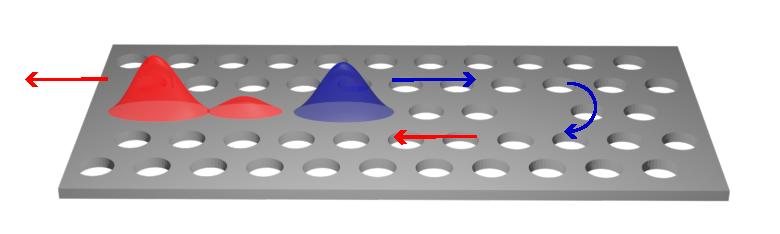
\includegraphics[width=\linewidth]{figures/onesided_cavity.pdf}
    \caption{Schematic of a photonic crystal waveguide containing an L1 cavity (one missing hole) interacting with an incoming (blue) pulse producing a scattered (red) pulse.}
    \label{fig:onesided_wg}
\end{figure}

\section{Continuous Fock States}
We can describe the traveling quantum pulse as occupying a collection of bosonic modes. As an example, a traveling single photon can be defined as \cite{Ciccarello2018CollisionOptics}:
\begin{equation}
    |\psi\rangle=\int \mathrm{d} \nu \psi(\nu) w^{\dagger}(\nu)| \emptyset \rangle,
\end{equation}
where $w^{\dagger}(\nu)$ is the creation operator for a photon of frequency $\nu$ with units of $\sqrt{\mathrm{time}}$ and $\psi(\nu)$ defines the wavefunction of the pulse also with units of $\sqrt{\mathrm{time}}$. The field operators $w(\nu)$ and $w^\dagger(\nu)$ obey the commutator relations: $\comm{w(\nu)}{w^\dagger(\nu ')} = \delta(\nu - \nu ')$, $\comm{w(\nu)}{w(\nu ')} = 0$, and $\comm{w^\dagger(\nu)}{w^\dagger(\nu ')} = 0$. The free evolution of the pulse is given by the Hamiltonian:

\begin{equation}
    H_f= \hbar \int \mathrm{d} \nu \nu w^{\dagger}(\nu) w(\nu)
\end{equation}

If we consider some cavity or emitter system with annihilation and creation operators $a$ and $a^\dagger$ (note that a two-level system is equivalent to a cavity with a cutoff of one photon and a more appropriate symbol would here be $\sigma$), the interaction $H_{int}$ with the pulse is, under the assumption of the Rotating Wave Approximation, given as \cite{Ciccarello2018CollisionOptics}:

\begin{equation}
    H_{int} = \hbar \int \mathrm{d} \nu  \left(g(\nu) a^{\dagger} w(\nu) + g(\nu)^{*} a w^{\dagger}(\nu)\right)
\end{equation}
where $g(\nu)$ defines the coupling strength with each individual mode in the pulse. If we transform into an interaction picture with respect to $H_f$ we get (see appendix \ref{app:rotating}):

\begin{equation}
    \mathrm{e}^{i H_f t /\hbar} H_{int} \mathrm{e}^{-i H_f t /\hbar} = H_{int}(t) =  \hbar \int \mathrm{d} \nu \left(g(\nu) a^{\dagger} w(\nu) \mathrm{e}^{i\nu t} + g(\nu)^{*} a w^{\dagger}(\nu) \mathrm{e}^{-i\nu t}\right)
\end{equation}

Assuming that the interaction $g(\nu)$ is spectrally flat $g(\nu) = i \sqrt{\gamma/2 \pi}$, we can make a considerable simplification of the above interaction by introducing the Fourier transformed field operator: $w(t)=\frac{1}{\sqrt{2 \pi}} \int \mathrm{d} \nu w(\nu) e^{-i \nu t}$ with units of $1/\sqrt{\mathrm{time}}$. Note that the imaginary part in the coupling $g(\nu)$ is just one definition and that it is equally valid to define it as $g(\nu) = \sqrt{\gamma/2 \pi}$. Inserting $g(\nu) = i \sqrt{\gamma/2 \pi}$, we get:
\begin{equation}
    H_{int}(t) =  \hbar i \sqrt{\gamma} (a^\dagger w(t)-a w^\dagger(t) ) \label{eq:interaction}
\end{equation}
The implication of the above simplification is clear: the interaction is now only with a single (time) mode $w(t)$ at each time $t$. The single photon state can equivalently be defined as:

\begin{equation}
    \ket{\psi} = W^\dagger[\xi] \ket{\emptyset} = \int_{t_0}^{t_{end}} \mathrm{d}t \ \xi^{(1)}(t) w^\dagger(t) \ket{\emptyset} \label{eq:singlephoton}
\end{equation}
here $W^\dagger(\xi)$ creates a photon with the wavefunction $\xi^{(1)}(t)$ and by insertion we can show that $\xi^{(1)}(t) = \frac{1}{\sqrt{2 \pi}} \int \mathrm{d} \nu \psi(\nu) e^{-i \nu t} $. Here, $w^\dagger(t)$ is the creation operator for a photon at time $t$. The inner product $\bra{\psi} w^\dagger(t) w(t) \ket{\psi} = |\xi^{(1)}(t)|^2$ with units of inverse time thus gives the flux of photons at time $t$ and multiplied with a small timestep $\Delta t |\xi^{(1)}(t)|^2$ the probability of observing a photon at time $t$. 

We can take this picture of only interacting with a single mode at a time further and discretize the continuous fock state into time bins of width $\Delta t$. This amounts to defining new discretized annihilation and creation operators as \cite{Heuck2020Photon-photonCavities} (see also appendix \ref{app:rotating}):
\begin{equation}
     w(t_k) = w(k \Delta t) \rightarrow  \frac{w_k}{\sqrt{\Delta t}} \ \ \  \text{with} \ \comm{w_j}{w_k^\dagger} = \delta_{jk}
\end{equation}
where $w_k$ is the descritized (unitless) operator of the $k$th timebin and the factor of $1/\sqrt{\Delta t}$ assures the commutator relation in the limit of $\Delta t \rightarrow 0$. This means that the single photon continuous fock state becomes:
\begin{equation}
    \ket{\psi} = \int_{t_0}^{t_{end}} \mathrm{d}t \ \xi^{(1)}(t) w^\dagger(t) \ket{\emptyset}  \rightarrow 
\sum_{k=1}^N \sqrt{\Delta t} \xi(t_k) w_k^\dagger \ket{\emptyset} = \sum_{k=1}^N \sqrt{\Delta t} \xi(t_k) \ket{1_k} 
\end{equation}
where we introduced the binned photon state: $\ket{1_k}  = w_k^\dagger \ket{\emptyset}$. We now see that: $\bra{\psi} w_{k}^\dagger w_k \ket{\psi} = \Delta t \abs{\xi(t_k)}^2$ and the annihilation and creation operators $w_k$ and $w_k^\dagger$  now describes the probability of observing a photon in time bin $k$.
%The assumption of the interaction with the emitter/cavity being $g(\nu) = \sqrt{\gamma/2 \pi}$ can now also be motivated from a physical perspective. We expect the picture of only interacting with a single time-bin at a time to be valid if the field does not change significantly over the emitter/cavity. This is also known as the dipole approximation.

The interaction Hamiltonian equivalently becomes:
\begin{equation}
    H_{int}(t) =  \sum_k f_k(t) H_{k,int} = \sum_k f_k(t) i \hbar \sqrt{\gamma/\Delta t} (a^\dagger w_k - a w_k^\dagger) \label{eq:discretized_interaction}
\end{equation}
where we defined:
\begin{equation}
f_k(t) = \begin{cases}
          1, & \text{if } t_k < t <t_k+\Delta t  \\
          0, & \text{otherwise}
\end{cases} = \Theta(t - t_k) - \Theta(t - (t_k + \Delta t)) \label{eq:fk}    
\end{equation}
where $\Theta$ is the heaviside function and $H_{k,int} = i \hbar \sqrt{\gamma/\Delta t} (a^\dagger w_k - a w_k^\dagger)$. The Hamiltonian is thus constant within each time-bin, which reduces the numerical complexity significantly. It also allows for an intuitive mental picture: We are moving a conveyor belt of photon bins and letting one bin of the belt interact with the system at a time. This is also illustrated in Fig.~\ref{fig:conveyor}. Throughout the thesis, we will use the subscript $k$ on a Hamiltonian $H_k$ to denote that it follows the form in \eqref{eq:discretized_interaction}, and it is thus understood that the Hamiltonian is changing with each timestep $k$, but is constant WITHIN each timestep.

\begin{figure}
    \centering
    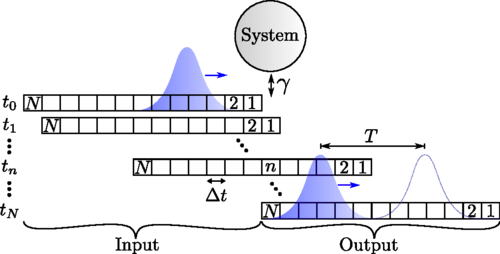
\includegraphics[width = 0.5 \linewidth]{figures/medium (1).png}
    \caption{Illustration of the interaction with one part of the pulse at a time. In the top row, an initial continuous fockstate is divided across N bins. At the subsequent timesteps labeled $t_i$, bin number $i$ interacts with the system. Once all bins have interacted with the system, the state in the bins is the output state. Image taken from ref. \cite{Heuck2020Photon-photonCavities}}
    \label{fig:conveyor}
\end{figure}


\section{Scattering on Onesided Cavity \label{sec:onephoton_scat}}
In the previous section, we introduced the time-bin formalism, and in this section, we are going to use it to derive the dynamics of a single photon pulse scattering on a single-sided cavity. Such a system can also be seen in Fig.~\ref{fig:onesided_wg}, where a photonic crystal waveguide carries a quantum pulse that interacts with a one-sided cavity. The differential equations governing the dynamics are defined from the Hamiltonian in eq.~\ref{eq:discretized_interaction}. Since the Hamiltonian is constant within each time-bin, we can describe the evolution from time-bin $n-1$ to $n$ by the unitary evolution \cite{Heuck2020Photon-photonCavities}:
\begin{equation}
    U_n = U(t_{n-1},t_{n}) = \exp \left(- \int_{t_{n-1}}^{t_{n-1}+\Delta t} \frac{i}{\hbar} H_{int}(t^{\prime}) d t^{\prime} \right)  =\exp \left(-\frac{i}{\hbar} H_{k,int} \Delta t\right)=\sum_{m=0}^{\infty} \frac{1}{m !}\left(-\frac{i}{\hbar} H_{n,int} \Delta t\right)^m
\end{equation}
which thus relates the state at time $t_{n-1}$ to the state at time $t_n$ as: $U_n \ket{\psi_{n-1}} = \ket{\psi_n}$, where $\ket{\psi_k}$ denote the state at time $t_k$. Up to first order in $\Delta t$, $U_n$ is given as:
\begin{equation}
    U_n \approx 1+\sqrt{\gamma \Delta t}\left(a^{\dagger} w_n-a w_n^{\dagger}\right)-\frac{\gamma}{2} \Delta t a^{\dagger} a w_n w_n^{\dagger} \label{eq:unitaryevolution}
\end{equation}
We consider the initial state being zero photons in the cavity and a one photon wavepacket (we use the Ket $\ket{\emptyset}$ to describe the vacuum of the waveguide, whereas $\ket{0}$ to describe the vacuum of the cavity):
\begin{equation}
    \left|\psi_0\right\rangle = \sum_{k=1}^N \sqrt{\Delta t} \xi(t_k) \ket{0} \ket{1_k} \label{eq:initial_single}
\end{equation}
The updated state after the first interaction with the time-bin is then given as:
\begin{equation}
    \ket{\psi_1} = U_1 \ket{\psi_0} = \sum_{k=2}^N \sqrt{\Delta t} \xi(t_k) \ket{0} \ket{1_k} + \sqrt{\Delta t} \xi(t_1) \ket{0} \ket{\mathbf{1}_1} + \sqrt{\gamma}  \Delta t \xi(t_1) \ket{1}\ket{\emptyset}
\end{equation}
where we have introduced bold enumeration $\ket{\mathbf{1}_1}$ for the time-bins that have passed the cavity to make the bookkeeping easier. We also introduce $\psi_1(t_1) =\sqrt{\gamma}  \Delta t \xi(t_1)$ as the amplitude of the cavity excitation at time $t_1$. After step two, we then have:

\begin{equation}
\begin{aligned}
    \ket{\psi_2} = U_2 \ket{\psi_1} &= \sum_{k=3}^N \sqrt{\Delta t} \xi(t_k) \ket{0} \ket{1_k} + \sum_{k=1}^2 \sqrt{\Delta t} \xi(t_k) \ket{0} \ket{\mathbf{1}_k} - \sqrt{\gamma \Delta t} \psi_1(t_1) \ket{0}\ket{\mathbf{1}_2} \\
    & + \sqrt{\gamma}  \Delta t \xi(t_2) \ket{1}\ket{\emptyset} - \frac{\gamma}{2} \Delta t \psi(t_1) \ket{1}\ket{\emptyset} + \psi_1(t_1) \ket{1}\ket{\emptyset}
\end{aligned}
\end{equation}


We notice that we can collect the terms in front of the bins that have passed the cavity as $\xi_{out}(t_2) = \xi(t_2) - \sqrt{\gamma} \psi_1(t_1)$ and the amplitude of the cavity now reads: $\psi_1(t_2) = \psi_1(t_1) -\gamma/2 \Delta t \psi_1(t_1) + \sqrt{\gamma}\Delta t \xi(t_2)$. We can generalize these update rules as:
\begin{equation}
    \psi_1(t_{n+1}) = \psi_1(t_n) -\frac{\gamma}{2} \Delta t \psi_1(t_n) + \sqrt{\gamma}\Delta t \xi(t_{n+1}) \label{eq:updaterule} 
\end{equation}
\begin{equation}
    \xi_{out}(t_{n+1}) = \xi(t_{n+1}) - \sqrt{\gamma} \psi_1(t_{n}) 
\end{equation}
If we take the limit of $\Delta t \rightarrow 0$, we have $t_{n+1} = t_n$ and rearranging eq.~\ref{eq:updaterule}, we arrive at the differential equation:
\begin{equation}
    \frac{\psi_1(t_{n+1}) - \psi_1(t_n)}{\Delta t} \xrightarrow[]{\Delta t \rightarrow 0} \frac{d \psi_1(t)}{d t}  = -\frac{\gamma}{2} \psi_1(t) + \sqrt{\gamma} \xi^{(1)}(t)
\end{equation}
Solving the differential equation then gives access to the scattered or output field by the input-output relation $\xi_{out}(t) = \xi^{(1)}(t) - \sqrt{\gamma} \psi_1(t)$. 

In a more realistic case, we could add a detuning between the pulse and the cavity $\delta = \omega_{c} - \omega_{w}$, where $\omega_{c}$ is the cavity frequency and $\omega_{w}$ is the central frequency of the waveguide pulse. As shown in the appendix \ref{app:rotating}, moving into the rotating frame would correspond to adding the term $\delta a^\dagger a$ to the Hamiltonian in eq.~\eqref{eq:discretized_interaction}. To get the correct equations of motion, we would then have to rederive the above equations. Luckily, in the above case, the detuning term is simple and just adds a phase term $-i\delta \Delta t a^\dagger a$ to the unitary in eq.~\eqref{eq:unitaryevolution}, which in turn just adds a phase term in the equation of motion:
%Note that due to the pulse's finite temporal shape, it contains multiple frequencies. However, as shown in appendix \ref{app:rotating}, if one assumes cavity frequencies in the visible spectrum (THz) regime and pulse durations of around several $\mathrm{ps}$, then the frequency spread (GHz) is negligible. Thus, a
\begin{equation}
    \frac{d \psi_1(t)}{d t}  = -(i \delta_a +\frac{\gamma}{2}) \psi_1(t) + \sqrt{\gamma} \xi^{(1)}(t) \label{eq:single_EOM}
\end{equation}
One could, however, easily imagine that adding more complicated terms to the Hamiltonian would require a more cumbersome rederivation. Indeed, as we shall see in the next section, an initial state consisting of two photons leads to additional possible paths of a photon, resulting in significantly more complex equations of motion. Automating this process to be less tedious is one of the main motivations behind the numerical method introduced in Chapter \ref{ch3}.

\section{Two-photon Continuous Fockstates \label{sec:twophoton_continuous}}
Before we introduce our new numerical method, let us, however, get some intuition for traveling two-photon states and why they complicate the scattering. 
It is straightforward to extend the single-photon state defined in eq.~\eqref{eq:singlephoton} to a two-photon continuous state as \cite{Baragiola2012N-PhotonSystem}:

\begin{align}
\frac{1}{\sqrt{2}}\left[W^\dagger[\xi]\right]^2| \emptyset \rangle = \frac{1}{\sqrt{2}} \int_{t_0}^{t_{end}} d t^{\prime} \int_{t_0}^{t_{end}} d t \ \xi^{(2)}(t,t^{\prime}) w^\dagger(t) w^\dagger\left(t^{\prime}\right)|\emptyset \rangle  
\end{align}
where $\xi^{(2)}(t,t') = \xi^{(1)}(t)\xi^{(1)}(t')$ is the two-photon wavefunction. The state is now defined over two times, describing the probability of observing a photon at time $t$ and another at time $t'$. In this case, the two-photon wavefunction is a product state, and both probabilities are described by the same single-photon wavefunction $\xi^{(1)}(t)$. This will, in general, not be the case. However, one can always expand the two-photon wavefunction in terms of products of one-photon wavefunctions via a Singular Value Decomposition (SVD) as \cite{Yang2022DeterministicSystems}:
\begin{equation}
    \xi^{(2)}(t,t') = \sum_i \lambda_i \phi_i(t) \phi_i(t') \label{eq:SVD}
\end{equation}
where $\phi_i(t)$ are orthonormal basis functions and if we have a normalized wavefunction $\sum_i\lambda_i^2 = 1$. In the above product state, we would thus have $\lambda_1^2 = 1$, i.e., the two-photon wavefunction contains only a product state of two single-photon states. It is now also clear that the wavefunction fulfills $\xi^{(2)}(t,t') = \xi^{(2)}(t',t)$, as expected for bosons. When discretizing the photon into bins, we thus only need $\approx N^2/2$ bins. This can be seen by:
\begin{align}
\frac{1}{\sqrt{2}} \left[W^\dagger(\xi)\right]^2|\emptyset \rangle &= \frac{1}{\sqrt{2}} \int_{t_0}^{t_{end}} d t^{\prime} \int_{t_0}^{t_{end}} d t \ \xi^{(2)}(t,t^{\prime}) w^\dagger(t) w^\dagger\left(t^{\prime}\right)|\emptyset \rangle \\
& \rightarrow \frac{1}{\sqrt{2}} \sum_{i=1}^N \sum_{k=1}^N   \Delta t \xi^{(2)} \left (t_i,t_k\right ) w_i^\dagger w_k^{\dagger}|\emptyset\rangle \\
& = \frac{1}{\sqrt{2}} \sum_{i=1}^N \sum_{k \neq i}^N \Delta t \xi^{(2)} \left (t_i,t_k\right) w_i^{\dagger} w_k^{\dagger}|\emptyset\rangle + \frac{1}{\sqrt{2}} \sum_{i=1}^N \Delta t \xi^{(2)} \left (t_i,t_i\right )w_i^\dagger w_i^\dagger\left|\emptyset\right\rangle \\
& =\frac{2}{\sqrt{2}} \sum_{i=1}^N \sum_{k>i}^N \Delta t \xi^{(2)} \left (t_i,t_k\right )\left|1_{t_i} 1_{t_k}\right\rangle + \sum_{i=1}^N \Delta t \xi^{(2)} \left (t_i,t_i\right ) \left|2 t_i\right\rangle \\
& =\sqrt{2} \sum_{i=1}^N \sum_{k > i}^N \Delta t \xi^{(2)}\left (t_i,t_k\right ) \mid 1_{t_i} 1_{t_k}\rangle + \sum_{i=1}^N \Delta t \xi^{(2)}\left (t_i,t_i\right )\left|2 t_i\right\rangle
\end{align}
This will be important in the next chapter when we want to represent the state numerically. In deriving the equations of motion, we will be taking $\Delta t \rightarrow 0$ (and thus also $N \rightarrow \infty$), and the diagonal containing two photons in the same time-bin will be vanishingly small and can thus be omitted. This will not be the case in the numerical representation, but for now, we can take the initial state to be $\ket{\psi}_0 = \sqrt{2} \sum_{i=1}^N \sum_{k > i}^N \xi_2\left (t_i,t_k\right ) \ket{0} \ket{1_{i} 1_{k}} $. Applying the unitary operator in eq.~\eqref{eq:unitaryevolution} then leads to the following state after the first timestep:
\begin{equation}
    \ket{\psi_1} = U_1 \ket{\psi_0} = \ket{\psi_0} + \sqrt{2 \gamma \Delta t} \sum_k 
\xi(t_1,t_k) \Delta t \ket{1} \ket{\emptyset,1_k} = \ket{\psi_0} + \ket{\psi_{abs,1}}
\end{equation}
In the subsequent timestep, the complexity grows immediately as multiple processes can take place. We can break it into two scenarios; absorption of the next photon bin corresponding to $U_2 \ket{\psi}_0$ and evolution of the absorbed photon in the cavity  $U_2 \ket{\psi}_{abs,1}$:
\begin{equation}
    \ket{\psi_2} = U_2 \ket{\psi_1} =U_2 \ket{\psi_0} + U_2 \ket{\psi}_{abs,1}  
\end{equation}
The absorption of the next bin is simple:
\begin{equation}
    U_2 \ket{\psi_0} =  \ket{\psi_0} + \sqrt{2 \gamma \Delta t} \sum_k 
\xi(t_2,t_k) \Delta t \ket{1} \ket{\emptyset,1_k}
\end{equation}
whereas for the already absorbed photon, we have terms corresponding to the reemission of a photon, reflection of an input photon, and absorption of another photon:
\begin{align}
 U_2 \ket{\psi}_{abs,1} &= \ket{\psi}_{abs,1} +  \sqrt{2} \gamma \Delta t^2 \xi(t_1,t_2) \ket{2} \ket{\emptyset,\emptyset} - \sqrt{2} \gamma \Delta t \sum_k 
\xi(t_1,t_k) \Delta t \ket{0} \ket{\mathbf{1}_2,1_k}\\ &- \sqrt{2 \gamma \Delta t} \gamma \Delta t /2 \sum_{k \neq 2} 
\xi(t_1,t_k) \Delta t \ket{1} \ket{\emptyset,1_k} 
 - \sqrt{\gamma \Delta t} \gamma \Delta t \xi(t_1,t_2) \Delta t \ket{1} \ket{\emptyset,1_2} 
\end{align}
From here, it is easy to imagine the many branches appearing. A full derivation is not within the scope of this thesis. Instead, we state the results of previous derivations \cite{Korsgaard2021Few-PhotonThesis} leading to the equations of motion:

\begin{equation}
\begin{array}{lr}
\dot{\psi}_2\left(\tilde{t}_n\right)=\sqrt{2} \psi_1^{(2)}\left(\tilde{t}_n\right) \tilde{\xi}_{\text {in }}\left(\tilde{t}_n\right)-\psi_2\left(\tilde{t}_n\right)-2 i \tilde{\delta} \psi_2\left(\tilde{t}_n\right), & \psi_2(0)=0 \\
\dot{\psi}_1^{(2)}\left(\tilde{t}_n\right)=\sqrt{2} \tilde{\xi}_{\text {in }}\left(\tilde{t}_n\right)-\frac{1}{2} \psi_1^{(2)}\left(\tilde{t}_n\right)-i \tilde{\delta} \psi_1^{(2)}\left(\tilde{t}_n\right), & \psi_1^{(2)}(0)=0 \\
\dot{\psi}_1^{(1)}\left(\tilde{t}_m, \tilde{t}_n\right)=\tilde{\xi}_{\text {in }}\left(\tilde{t}_n\right)-\frac{1}{2} \psi_1^{(1)}\left(\tilde{t}_m, \tilde{t}_n\right)-i \tilde{\delta} \psi_1^{(1)}\left(\tilde{t}_m, \tilde{t}_n\right), & \psi_1^{(1)}\left(\tilde{t}_m, \tilde{t}_m\right)=0 \\
\dot{\psi}_1^{(0)}\left(\tilde{t}_m, \tilde{t}_n\right)=-\frac{1}{2} \psi_1^{(0)}\left(\tilde{t}_m, \tilde{t}_n\right)-i \tilde{\delta} \psi_1^{(0)}\left(\tilde{t}_m, \tilde{t}_n\right), & \psi_1^{(0)}\left(\tilde{t}_m, \tilde{t}_m\right)=1
\end{array} \label{eq:twophotonEOM}
\end{equation}
where $\psi_2\left(\tilde{t}_n\right)$ describes the amplitude of states $\ket{2}\ket{\emptyset}$, $\psi_1^{(2)}\left(\tilde{t}_n\right)$ describes the amplitude of states $\ket{1}\ket{1_k}$, $\psi_1^{(1)}\left(\tilde{t}_m, \tilde{t}_n\right)$ describes the amplitude of states $\ket{1}\ket{\mathbf{1}_k}$ coming from reabsorption processes, and $\psi_1^{(0)}\left(\tilde{t}_m, \tilde{t}_n\right)$ describes the amplitude of states $\ket{1}\ket{\mathbf{1}_k}$ emission processes. Also, $\tilde{t_n} = \gamma t_n$, $\tilde{\delta} = \delta/\gamma$ has been defined and $\dot{A}$ here denotes differentiation of $A$ with regards to $t_n$. The input distribution is assumed to be a product state $\xi_2(t_1,t_2) = \xi_\mathrm{in}(t_1)\xi_\mathrm{in}(t_2)$ with $\tilde{\xi_\mathrm{in}} = \xi_\mathrm{in}/\sqrt{\gamma}$. The output relation is given as:
\begin{equation}
\begin{aligned}
\tilde{\xi}_{\text {out }}^{(2)}\left(\tilde{t}_m, \tilde{t}_n\right) & =\tilde{\xi}_{\text {in }}\left(\tilde{t}_m\right) \tilde{\xi}_{\text {in }}\left(\tilde{t}_n\right)+\frac{1}{\sqrt{2}}\left[\sqrt{2} \psi_2\left(\tilde{t}_m\right) \psi_1^{(0)}\left(\tilde{t}_m, \tilde{t}_n\right)+\psi_1^{(2)}\left(\tilde{t}_m\right) \psi_1^{(1)}\left(\tilde{t}_m, \tilde{t}_n\right)\right. \\
& \left.-\psi_1^{(2)}\left(\tilde{t}_m\right) \tilde{\xi}_{\text {in }}\left(\tilde{t}_n\right)-\psi_1^{(2)}\left(\tilde{t}_m\right) \psi_1^{(0)}\left(\tilde{t}_m, \tilde{t}_n\right) \tilde{\xi}_{\text {in }}\left(\tilde{t}_m\right)-\sqrt{2} \psi_1^{(1)}\left(\tilde{t}_m, \tilde{t}_n\right) \tilde{\xi}_{\text {in }}\left(\tilde{t}_m\right)\right]
\end{aligned}
\end{equation}
with $\tilde{\xi}_{\text {out }}^{(2)}\left(\tilde{t}_m, \tilde{t}_n\right) = \xi_{\text {out }}^{(2)}\left(\tilde{t}_m, \tilde{t}_n\right)/\gamma$. Notice that the differential equations for $\psi_1^{(1)}\left(\tilde{t}_m, \tilde{t}_n\right)$ and $\psi_1^{(0)}\left(\tilde{t}_m, \tilde{t}_n\right)$ depend on two times and thus need to be solved for $N$ different initial conditions where $N$ is some binning in time. This complex hierarchy of multiple coupled differential equations has to be solved motivates a computer-assisted approach, where the derivation and subsequent solution are automatic. Any additions to the Hamiltonian, such as a non-linearity, would also necessitate a rederivation. Indeed, even considering a two-level emitter instead of a cavity would require new derivations as the emitter cannot be excited twice (the state $\ket{2}$ is not possible). In the following chapter, we discuss how we can automate this process by representing the Hamiltonian numerically and solving the resulting differential equation.








\chapter{WaveguideQED.jl \label{ch3}}
This chapter will introduce the numerical framework implemented in \href{https://qojulia.github.io/WaveguideQED.jl/dev/}{WaveguideQED.jl}. The implementation is based on the time-binned continuous fockstate formalism introduced in Chapter 2. We show that it correctly recovers equations of motion in the limit of $\Delta t \rightarrow 0$ by doing a convergence study. Furthermore, we introduce Lazy Operator data structures, which are used in our software implementation to enhance performance.   

\section{Numerical Representation of One-photon States} \label{sec:onephoton_numerical}
In ch.~\ref{ch2}, we used the time-binned picture to derive the equations of motion for a single-photon scattering on a cavity. Ultimately, we took the limit of $\Delta t \rightarrow 0$ meaning infinitesimally small bins, thus restoring the continuous fockstate. In this section, however, we will keep the time-binned photon representation and show how we can obtain equivalent results numerically. 

If we consider a continuous photon state in $N$ bins with no more than a single photon, we will need a vector of size $N+1$ to represent it (plus one because we also need to represent vacuum $\ket{\emptyset}$). This is illustrated in Fig.~\ref{fig:onephoton_representation} with $N=5$. In this truncated Hilbert space, the effect of applying the operator $w_3^\dagger$ is then given as
\begin{equation}
    w_3^\dagger \ket{\psi} = \begin{pmatrix}
        0 & 0 & 0 & 0 & 0 & 0 \\
        0 & 0 & 0 & 0 & 0 & 0 \\
        0 & 0 & 0 & 0 & 0 & 0 \\
        1 & 0 & 0 & 0 & 0 & 0 \\
        0 & 0 & 0 & 0 & 0 & 0 \\
        0 & 0 & 0 & 0 & 0 & 0 \\
    \end{pmatrix} \cdot \begin{pmatrix}
        \textcolor{red}{\psi_\emptyset} \\
        \psi_1 \\
        \psi_2 \\
        \psi_3 \\
        \psi_4 \\
        \psi_5
    \end{pmatrix} = \begin{pmatrix}
        0 \\
        0 \\
        0 \\
        \textcolor{red}{\psi_\emptyset} \\
        0 \\
        0
    \label{eq:operator_matrix} \end{pmatrix} 
\end{equation}
here, $\psi_i$ denotes the value stored in element $i$ (starting from zero to represent vacuum and the subsequent $N$ elements to represent the single photon excitation). Figure \ref{fig:onephoton_representation} also shows the effect of applying the operator $w_3^\dagger$: Move the element in $\ket{\emptyset}$ to the element in time-bin $3$. In the sketch, we only denote non-zero changes with the arrow; therefore, it is understood that all other elements are zero after the operation. Note that Fig~\ref{fig:onephoton_representation} shows the physical effect of applying $w_3^\dagger$. Numerically, the result of applying such operations is, as we shall see, often stored in another vector \code{dpsi}, and a more accurate representation would therefore be to draw an arrow between the input vector \code{psi} and the vector that stores the resulting state \code{dpsi}. For the sake of simplicity, we omit this extra step in all illustrations.  
\begin{figure}[H]
    \centering
    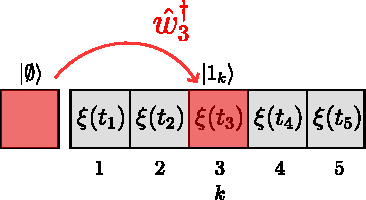
\includegraphics[width=0.5 \linewidth]{figures/one_photon_create.pdf}
    \caption{A numerical representation of the one-photon state and the effect of applying the creation operator $w_3^\dagger$. We only denote non-zero changes with the arrow; therefore, it is understood that all other elements are zero after the operation. Numerically, another vector \code{dpsi} would be used to store the result of the calculation. For simplicity, this vector is not shown either.}
    \label{fig:onephoton_representation}
\end{figure}
To solve the scattering problem, we combine the state of the waveguide with the state of the cavity by a tensor product. Since we only consider a total of one excitation, we can truncate the Hilbert space of the cavity to $\{ \ket{0},\ket{1} \}$ or equivalently a vector of length two. An arbitrary state of the waveguide and cavity can thus be described as:
\begin{equation}
    \ket{\psi} = \ket{0} \otimes \left( A_0 \ket{\emptyset}+ \sum_{k=1}^N \sqrt{\Delta t} \xi_0(t_k) \ket{1_k} \right ) + \ket{1} \otimes \left( A_1 \ket{\emptyset}+ \sum_{k=1}^N \sqrt{\Delta t} \xi_1(t_k) \ket{1_k} \right ) 
\end{equation}
where $A_0$, $A_1$, $\xi_0(t_k)$, $\xi_1(t_k)$ are the elements stored in a vector of the same structure as in Fig.~\ref{fig:onephoton_representation}. After the tensor product, we thus have a vector of length $2\cdot(N+1)$. We can here associate the first $N+1$ elements with the cavity being empty: $\ket{0}$ and the last $N+1$ with the cavity having one photon: $\ket{1}$. A numerical representation of this state can be seen in Fig.~\ref{fig:cavity_create}. The action of the operators $a^\dagger w_k$ and $a w_k^\dagger$ making up the interaction Hamiltonian in eq.~\eqref{eq:discretized_interaction} with $k = 3$ is also shown. Again, the interpretation is clear, $a^\dagger w_k$ removes an excitation from time-bin $k$ and places it in the cavity mode, while $a w_k^\dagger$ does the opposite. 


 
\begin{listing}[H]
\begin{minted}[
frame=lines,
framesep=2mm,
baselinestretch=1.2,
bgcolor=LightGray,
fontsize=\small,
linenos
]{julia}
function dpsi!(dpsi,psi,p,t)
    y,d,nsteps,dt = p
    timeindex = round(Int,t/dt,RoundDown) + 1
    dpsi .= 0
    dpsi[2+nsteps] = sqrt(y/dt)*psi[1+timeindex] - im*d*psi[2+nsteps]
    dpsi[1+timeindex] = -sqrt(y/dt)*psi[2+nsteps]
end
\end{minted}
\caption{Function to calculate the derivative, given by applying $- i H(t_k) = - i \delta_a a^\dagger a + \sqrt{\gamma/dt}(a^\dagger w_k - a w_k^\dagger)$ to the state {\fontfamily{pcr}\selectfont psi} and saved in {\fontfamily{pcr}\selectfont dpsi}.}
\label{ls:derivative}
\end{listing}
\begin{figure}
    \centering
    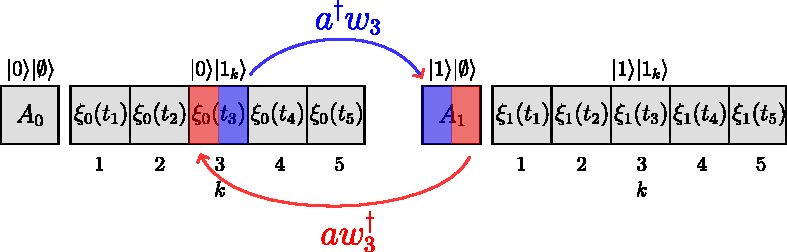
\includegraphics[width=0.8 \linewidth]{figures/cavity_destroy_create.pdf}
    \caption{A numerical representation of the combined state of a one photon state in the waveguide $\ket{1_k}$ and a cavity containing zero $\ket{0}$ or one photon $\ket{1}$. The effect of applying the operators $a^\dagger w_3$ and $a w_3^\dagger$ is also shown with blue and red arrows, respectively. }
    \label{fig:cavity_create}
\end{figure}

Based on these definitions of the operators, it is possible to set up a very simple simulation of the dynamics. The governing equation is Schr{\"o}dinger's equation $\frac{\partial}{\partial t} \ket{\psi} = - i H \ket{\psi}$, and in Code Sample \ref{ls:derivative} we implement a function in Julia that returns the derivate \code{dpsi} by applying $- i H(t_k) = - i \delta_a a^\dagger a + \sqrt{\gamma/dt}(a^\dagger w_k - a w_k^\dagger)$ to {\fontfamily{pcr}\selectfont psi} as depicted in Fig.~\ref{fig:onephoton_representation}. Notice that {\fontfamily{pcr}\selectfont timeindex} determines which bin the waveguide operators $w_k$ and $w_k^\dagger$ address. Line 5 updates $\ket{1}\ket{\emptyset}$ with $\sqrt{\gamma/\Delta t} a^\dagger w_k$ and $- i \delta_a a^\dagger a$. Line 6 updates $\ket{0}\ket{1_k}$ with $-\sqrt{\gamma/\Delta t} a w_k^\dagger$. This derivative function can then be passed to a differential equation solver to get the dynamics.

In the following, we consider a Gaussian input state with the wavefunction $\xi^{(1)}(t)$ defined as 
\begin{equation}
    \xi^{(1)}(t) = \sqrt{\frac{2}{\sigma}} \left(\frac{\log(2)}{\pi}\right)^{1/4} \exp\left(-\frac{2\log(2)(t-t_0)^2}{\sigma^2}\right) \label{eq:gaussian}
\end{equation}
In Code Sample \ref{ls:solver}, we use the derivative function from Code Sample \ref{ls:derivative} to solve the scattering of an input state with $\sigma = 1$ and $t_0 = 5$. We can compare the solution to the analytically obtainable solution to the equation of motion in eq.~\eqref{eq:single_EOM}. As shown in appendix \ref{app:analytical}, the analytical solution is given as:
\begin{equation}
    \xi^{(1)}_\mathrm{EOM}(t) =  \xi^{(1)}(t) - \sqrt{\gamma}\frac{\sqrt{\pi} e^{\frac{b^2}{4a}+bt_0}}{2\sqrt{a}}\left(\text{erf}\left(\frac{2a(t-t_0)-b}{2\sqrt{a}}\right) + \text{erf}\left(\frac{2at_0+b}{2\sqrt{a}}\right)\right) \label{eq:onephoton_analytical}
\end{equation}
with $a = 2 \log(2)/\sigma^2$ and $b = i \delta + \gamma/2$. The analytical solution is shown together with the numerical solution in Fig.~\ref{fig:singlephoton}. We see how the photon pulse is distorted from the interaction with the cavity. The dip in the scattered wavefunction around $t \approx 5.5/\gamma$ arises due to destructive interference between the reemitted field from the cavity and the reflected pulse. We will study this phenomenon in greater detail later. For now, it is important to notice the convergence in Fig.~\ref{fig:single_photon_convergence} showing that the two methods converge as the number of bins increases (meaning $\Delta t \rightarrow 0$). 

\begin{listing}[!ht]
\begin{minted}[
frame=lines,
framesep=2mm,
baselinestretch=1.2,
bgcolor=LightGray,
fontsize=\small,
linenos,
escapeinside=||,
mathescape=true
]{julia}
using DifferentialEquations
using LinearAlgebra
using PyPlot

#Define parameters
|$\gamma$|,|$\delta$|,dt = 1,0,0.1
times = 0:dt:10
N = length(times)
p = (|$\gamma$|,|$\delta$|,N,dt)

#Define input gaussian state with width s = 1 and arrival time t0=5
xi(t,s,t0) = sqrt(2/s)* (log(2)/pi)^(1/4)*exp(-2*log(2)*(t-t0)^2/s^2)
psi = zeros(ComplexF64,2*(N+1))
#Index 2:N+1 to adress $\ket{0}\ket{1_k}$ as in Fig. $\ref{fig:cavity_create}$
psi[2:N+1] .= sqrt(dt)*xi.(times,1,5)

#Define and solve ODE problem by giving initial state psi and differential operator dpsi!
prob = ODEProblem(dpsi!, psi, (times[1], times[end]+dt), p)
sol = solve(prob, OrdinaryDiffEq.DP5();reltol = 1.0e-8,abstol = 1.0e-10);
psi_out = sol[end][2:N+1]
\end{minted}
\caption{Code for solving scattering of single-photon pulse on onesided cavity. }
\label{ls:solver}
\end{listing}

\begin{figure}[H]
    \centering
    \subfloat[\label{fig:singlephoton}]{{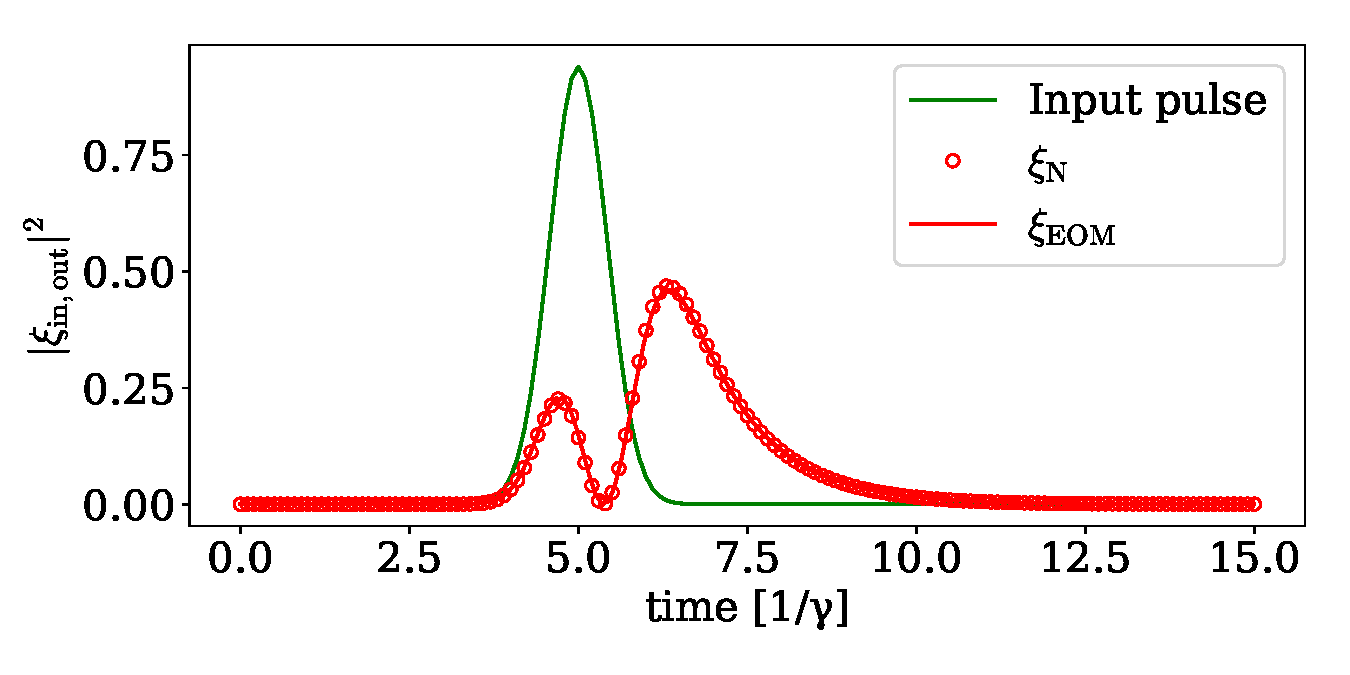
\includegraphics[width=0.49\textwidth]{figures/singlephoton.pdf}}}    \subfloat[\label{fig:single_photon_convergence}]{{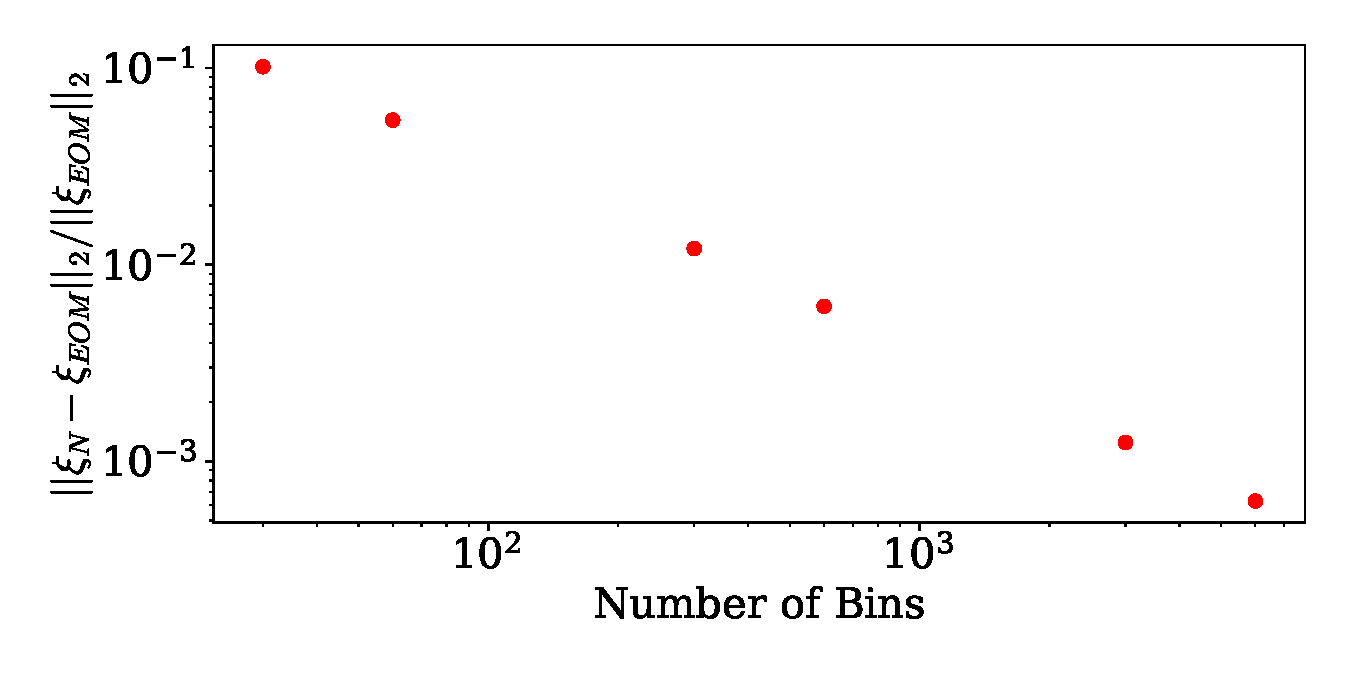
\includegraphics[width=0.49\textwidth]{figures/convergence.pdf} }}
    \caption{(a) The scattering of a Gaussian single-photon pulse defined in eq.~\eqref{eq:gaussian} on a single-sided cavity with $\sigma = 1$ and $t_0 = 5$. The solution to the equations of motion $\xi_\mathrm{EOM}$ from eq.~\eqref{eq:onephoton_analytical} is shown together with the numerical solution from the above code $\xi_\mathrm{N}$ (with a time-bin size of $\Delta t = 0.1/\gamma$). The two methods are seen to produce identical results. (b) Convergence plot showing the relative error in the L2-norm $||f||_2 = \int_{-\infty}^\infty |f(t)|^2 d t $ between the equation of motion solution and the numerical solution. }
\end{figure}

The above numerical implementation is very simple and fast, but it is also hardcoded to solve one specific problem. This is not the ultimate goal of the implementation, as we want it to be flexible and able to solve many different waveguide QED problems. The natural extension is to implement the operators $a$, $a^\dagger$, $w_k$, and $w_k^\dagger$ as matrices and then combine them through the tensor product $\otimes$. In the next section, we show how this can be done in 
\href{https://qojulia.org/}{QuantumOptics.jl} a package for simulating Quantum Optics in Julia \cite{Kramer2018QuantumOptics.jl:Systems}.

\section{Sparse Operators \label{sec:sparseoperators}}
In this section, we show how to implement the waveguide operators $w_k$ and $w_k^\dagger$ as sparse matrices in \href{https://qojulia.org/}{QuantumOptics.jl}. As we shall see the cost of allocating memory for these matrices quickly becomes a limiting factor as the size of the problem grows. Lazy operators, introduced in section \ref{sec:lazyoperators} is the solution. For now, it is, however, still instructive to consider the more straightforward case of sparse matrices. 

In the truncated Hilbert space of only a single-photon time-binned state, we can define waveguide operators according to the transition they represent $w_k = \ket{\emptyset} \bra{1_k}$ and $w_k^\dagger = \ket{1_k} \bra{\emptyset}$. In Julia, using \href{https://qojulia.org/}{QuantumOptics.jl}, this can be accomplished by the code in Code Sample \ref{ls:sparseoperators}. Here, we define the basis of the waveguide \code{bw} as a GenericBasis, which is an object subsequently used to define kets belonging to that Hilbert space. In this case, the most important property of the Basis is that it contains the size of Hilbert space ($N+1$, where $N$ is the number of bins). $w_k$ is then initialized by taking the tensor product between the ket $\ket{\emptyset}$ and bra $\bra{1_k}$. $\ket{\emptyset}$ is defined from {\fontfamily{pcr}\selectfont basisstate(bw,1)}: A state belonging to the basis of waveguide {\fontfamily{pcr}\selectfont bw}, with the first element being occupied. Similarly,  $\bra{1_k}$ is then {\fontfamily{pcr}\selectfont dagger(basisstate(bw,1+timeindex))}, where {\fontfamily{pcr}\selectfont timeindex} here controls the time-bin we are addressing (in this case bin number one) and \code{dagger()} turns the ket into a bra. $w_k^\dagger$ is also just defined from applying \code{dagger()} to \code{w}.
\begin{listing}[H]
\begin{minted}[
frame=lines,
framesep=2mm,
baselinestretch=1.2,
bgcolor=LightGray,
fontsize=\small,
linenos,
escapeinside=||,
mathescape=true
]{julia}
dt = 0.1
times = 0:dt:10
N = length(times)
bw = GenericBasis(N+1)
timeindex = 1
w = basisstate(bw,1) |$\otimes$| dagger(basisstate(bw,1+timeindex))
wd = dagger(w)
\end{minted}
\caption{Code for creating waveguide operators $w$ and $w^\dagger$ as sparse matrices.}
\label{ls:sparseoperators}
\end{listing}
With the operators defined, we can combine them with a cavity through the tensor product $\otimes$ (in Julia: $\backslash \mathrm{otimes}$ followed by TAB). In Code Sample \ref{ls:combine}, we define the basis of the cavity \code{bc} containing at max one photon, the annihilation operator of this basis \code{a = destroy(bw)} and creation operator \code{ad = create(bw)}. These are then combined with the waveguide operators \code{w} and \code{wd} via tensor products to form $a^\dagger w_k$ and $a^\dagger w_k$, which finally can be combined to form the Hamiltonian $H = i \hbar \sqrt{\gamma/\Delta t}(a^\dagger w_k - a w_k^\dagger) +  \hbar \delta a^\dagger a$. Note that in all code and simulations, we set $\hbar = 1$.

\begin{listing}[H]
\begin{minted}[
frame=lines,
framesep=2mm,
baselinestretch=1.2,
bgcolor=LightGray,
fontsize=\small,
linenos,
escapeinside=||,
mathescape=true
]{julia}
bc = FockBasis(1)
a = destroy(bw)
ad = create(bw)
n = (ad*a) |$\otimes$| identityoperator(bw)
adw = ad |$\otimes$| w
wda = a |$\otimes$| wd
H = im*sqrt(|$\gamma$| / dt) *(adw - wda) + |$\delta$| * n 
\end{minted}
\caption{Code for combining cavity annihilation and creation operators $a$ and $a^\dagger$ with waveguide operators $w$ and $w^\dagger$.}
\label{ls:combine}
\end{listing}

In Code Sample \ref{ls:combine}, we, however, only created the Hamiltonian for the first timestep. Our Hamiltonian changes at each timestep, so we need to define a time-dependent problem. This is done in Code Sample \ref{ls:timedependent}, where we calculate the Hamiltonian for all timesteps in lines 1-8 and define a function that returns the Hamiltonian for the corresponding timestep in lines 9-12. In lines 14-16, we define the input state, in a similar fashion as in the previous section, except that we can now just combine the cavity and waveguide through the tensor product. Finally, say we are interested in the number of photons inside the cavity as a function of time, we can define the expectation-value function \code{na} in line 18. In line 19, we then solve the time-dependent problem by using our defined input state \code{psi\_in}, our function that returns our time-dependent Hamiltonian \code{Htime}, and our expectation value function \code{na}.

\begin{listing}[H]
\begin{minted}[
frame=lines,
framesep=2mm,
baselinestretch=1.2,
bgcolor=LightGray,
fontsize=\small,
linenos,
escapeinside=||,
mathescape=true
]{julia}
Hlist = Array{Operator}(undef,N)
for i in 1:N
    w = basisstate(bw,1) |$\otimes$| dagger(basisstate(bw,1+i))
    wd = dagger(w)
    adw = ad |$\otimes$| w
    wda = a |$\otimes$| wd
    Hlist[i] = im*sqrt(|$\gamma$| / dt) *(adw - wda) + |$\delta$|*n
end
function Htime(time,psi)
    timeindex = round(Int,time/dt,RoundDown)+1
    Hlist[timeindex]   
end

psi_waveguide = Ket(bw)
psi_waveguide.data[2:N+1] .=  sqrt(dt)*xi.(times,1,5)
psi_in = fockstate(bc,0) |$\otimes$| psi_waveguide

na(time,psi) = expect(n,psi)
_,n = timeevolution.schroedinger_dynamic(times, psi_in, Htime,fout=na)
\end{minted}
\caption{Code for defining a time-dependent problem in Julia.}
\label{ls:timedependent}
\end{listing}

In Fig.~\ref{fig:cavity_occupation}, we show the population in the cavity as a function of time for different detuning values $\delta$ as calculated by Code Sample \ref{ls:timedependent}. It is clear that as the detuning increases, the pulse absorption decreases. Comparing with Fig.~\ref{fig:singlephoton_wf}, where we show output wavefunction $\xi_{out}(t)$, we see that for larger detuning no dip appears. This is due to the lower cavity population, meaning less destructive interference and thus less distortion of the photon wavepacket. 

\begin{figure}[H]
    \centering
    \subfloat[\label{fig:cavity_occupation}]{{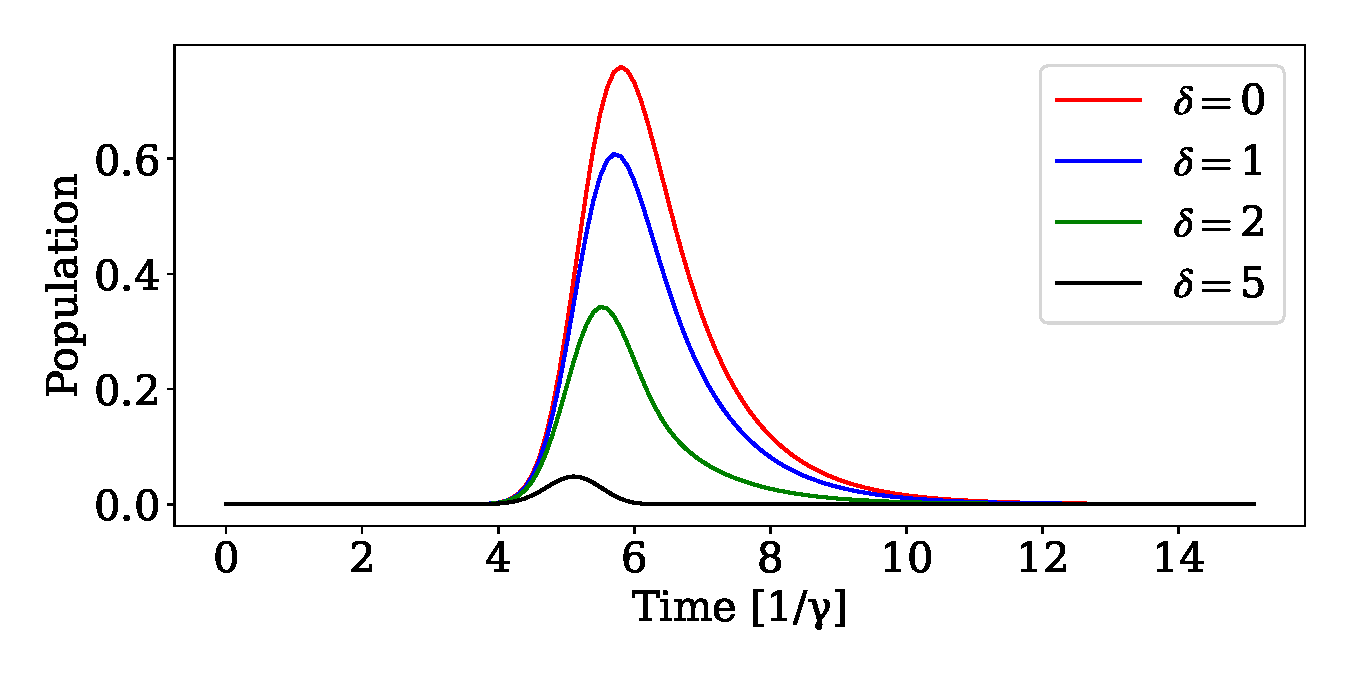
\includegraphics[width=0.49\textwidth]{figures/photon_number.pdf}}}    \subfloat[\label{fig:singlephoton_wf}]{{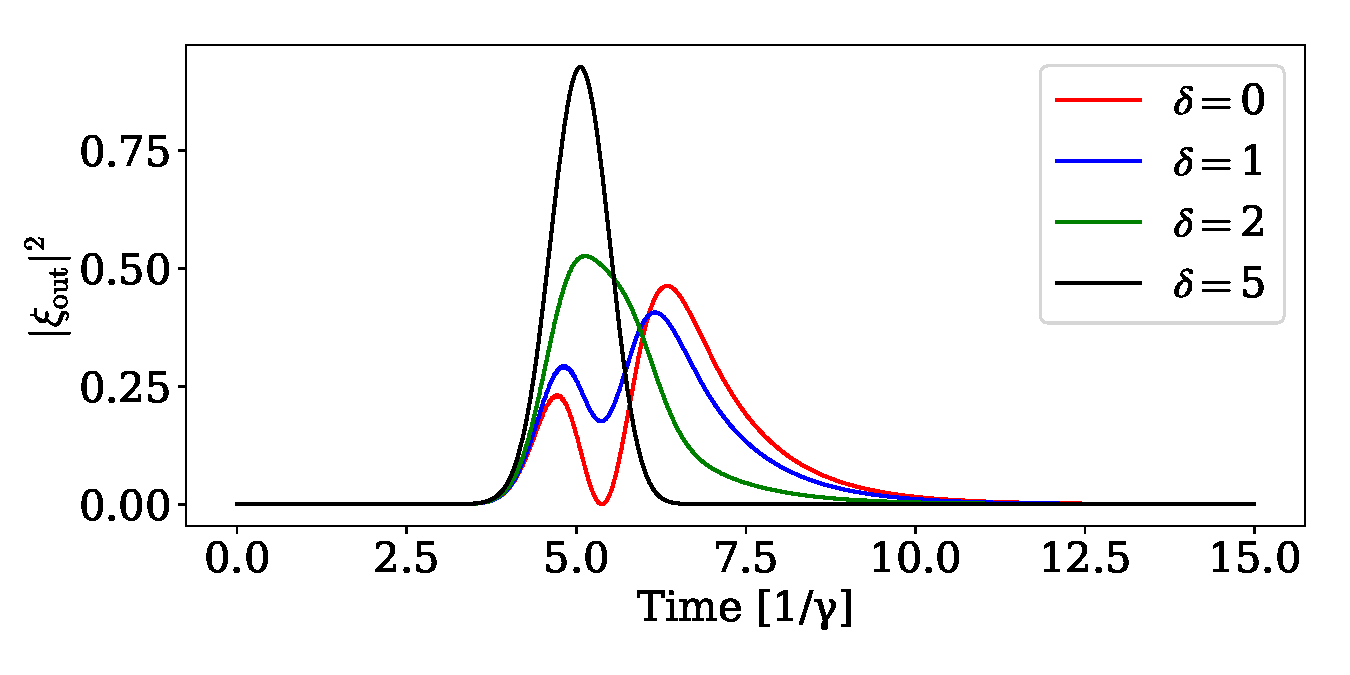
\includegraphics[width=0.49\textwidth]{figures/singlephoton_wavefunction.pdf} }}
    \caption{(a) Cavity photon population as a function of time for different values of detuning. (b) The scattered wavefunction as a function of time.}
\end{figure}


In this example, representing the operators $w_k$ and $w_k^\dagger$ as sparse matrices worked well since the Hilbert spaces we considered were small. In the next section, we will consider two-photon states, and as we shall see, the overhead associated with allocating these matrices quickly dominates the performance. 


\section{Numerical Representation of Two-photon States \label{sec:twophoton_numerical}}
As shown in chapter \ref{ch2}, the two-photon time binned state is given as:
\begin{equation}
    \ket{\psi} = \sqrt{2} \sum_{i=1}^N \sum_{k > i}^N \Delta t \xi_2\left (t_i,t_k\right ) \mid 1_{t_i} 1_{t_k}\rangle + \sum_{i=1}^N \Delta t \xi_2\left (t_i,t_i\right )\left|2 t_i\right\rangle
\end{equation}
Numerically, we need $N(N-1)/2 + N = N(N+1)/2$ bins to represent this state, where $N$ here is the number of bins of the single-photon state. The two-photon state is numerically a vector with $N(N+1)/2$ elements but is best visualized as a matrix, as shown in Fig.\ \ref{fig:twophoton_representation}. Note that the lower triangular part is not stored in memory due to the symmetry of the two-photon state. In the Figure, we also show how the creation operator $w_3^\dagger$ relates a one-photon state to a two-photon state, where the darker red square carries a factor of $\sqrt{2}$ since $w_3^\dagger \ket{1_3} = \sqrt{2}\ket{2_3}$. Here we imagine that we have a combined state of a single-photon state and a two-photon state, where the first element is the vacuum, the following $N$ elements are the single-photon state, and the last $N(N+1)/2$ elements are the two-photon state. In this truncated space, we can thus also write the creation operator as:
\begin{equation}
    w_k^\dagger = \ket{1_k} \bra{\emptyset} + \sum_{j < k} \ket{1_k,1_j} \bra{1_j} + \sum_{j > k} \ket{1_j,1_k} \bra{1_j} + \sqrt{2} \ket{2_k} \bra{1_k} 
\end{equation}
where the first term takes the vacuum to a single-photon state (as introduced earlier in sec.~\ref{sec:sparseoperators}), the second term takes a single-photon state at a previous time $j$ to a combined state of a photon at time $j$ and $k$, and the third term is similar and takes a future single-photon state at time $j$ and takes it into the combined state of a photon at time $j$ and $k$. The last term takes the single-photon at exactly time $k$ into the state with two photons in the same time bin $k$ and, thus, carries a factor of $\sqrt{2}$. 

\begin{figure}[H]
    \centering
    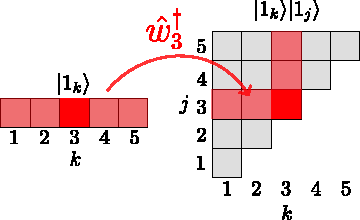
\includegraphics[width=0.6 \linewidth]{figures/twophoton.pdf}
    \caption{Numerical representation of a two-photon state together with the action of the waveguide operator $w_3^\dagger$ on a single-photon state. The darker red square has a factor of $\sqrt{2}$ to satisfy $w_3^\dagger \ket{1_3} = \sqrt{2} \ket{2_3}$ }
    \label{fig:twophoton_representation}
\end{figure}


Again this can be described as a sparse matrix. However, the sparse matrix is now of size $1+N+N(N+1)/2$. With $N=100$, this corresponds to a $5151 \mathrm{x} 5151$ matrix. If we now want to combine it with a cavity containing two photons to construct the operators $a^\dagger w_k$ and $a w_k^\dagger$, we have a tensor product between a $3\mathrm{x}3$ matrix and a $5151\mathrm{x}5151$ matrix. As shown in section \ref{sec:sparseoperators}, we construct and perform this tensor product for each timestep in the simulation. A quick benchmark reveals that this task quickly grows expensive. In Fig.~\ref{fig:createoperator_bench}, we compare the time spent creating the Hamiltonians and the time spent solving the actual differential equations. As the number of bins increases, we see that we spend most of the time just creating the Hamiltonian for the problem. The way the Hamiltonian change is, however, well known. We can exploit this and implement the operator instead as an object that executes a predefined function dependent on time, which mimics the behavior of doing the matrix multiplication. This is the core principle behind the Lazy Operators used in WaveguideQED.jl, which we will introduce in the next section. 


\begin{figure}[H]
    \centering
    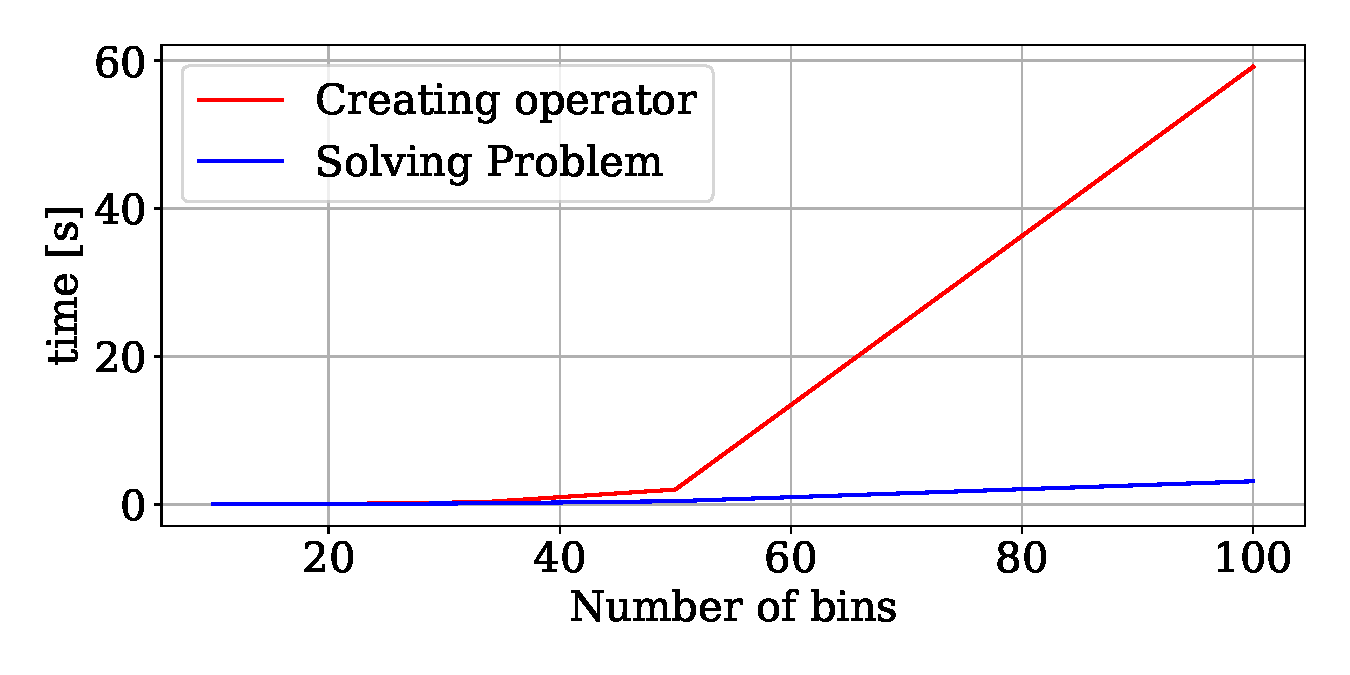
\includegraphics[width = 0.6 \linewidth]{figures/allocatingvssolving_bench.pdf}
    \caption{Comparison between time spend creating the Hamiltonians and solving the actual problem (here scattering of a two-photon pulse of a cavity with the Hamiltonian defined in eq.~\eqref{eq:discretized_interaction} ). It is evident that for more than $N\approx 60$, the majority of the computational time is taken up by just creating the Hamiltonians.}
    \label{fig:createoperator_bench}
\end{figure}


\section{Lazy Operators\label{sec:lazyoperators}}
Motivated by the significant overhead in creating the Hamiltonian for each time step, as seen in section \ref{sec:twophoton_numerical}, we want to represent the waveguide operator $w_k^\dagger$ as an object that can be applied to a ket and perform the already known operation. If we only consider a waveguide ket, the implementation is simple. In Code Sample \ref{ls:lazyoperator}, we define a structure representing the waveguide operator $w_k^\dagger$. \code{basis\_l} and \code{basis\_r} are objects that contain information about the Hilbert space and will become important when we later want to combine the structure with operators belonging to other Hilbert spaces. \code{factor} allows us to define arithmetic operations. As an example, $\beta * w_k^\dagger$, would update factor as: \code{factor = $\beta$ * factor}. Finally, \code{timeindex} allows us to change $k$ in each timestep. In the first timestep, we want to apply the operator $w_1^\dagger$, and we thus set \code{timeindex = 1}. In the next timestep, we then update \code{timeindex = 2} and so on.

\begin{listing}[H]
\begin{minted}[
frame=lines,
framesep=2mm,
baselinestretch=1.2,
bgcolor=LightGray,
fontsize=\small,
linenos,
escapeinside=||,
mathescape=true
]{julia}
abstract type WaveguideOperator{B1,B2} <: AbstractOperator{B1,B2} end
mutable struct WaveguideCreate{B1,B2,Np,idx} <: WaveguideOperator{B1,B2}
    basis_l::B1
    basis_r::B2
    factor::ComplexF64
    timeindex::Int
end
\end{minted}
\caption{Structure in Julia for defining Lazy Operator.}
\label{ls:lazyoperator}
\end{listing}

But how is the multiplication done? In Code Sample \ref{ls:multiplcation_code} lines 1-5, we show the multiplication routine for $w_k^\dagger$ on a state that contains a single photon. The routine updates the vector result as: \code{result = factor * $\alpha$ * $w_k^\dagger$ * b +  $\beta$ * result} (note the presence of \code{factor}). The routine for doing two-photon multiplication is more complex and can be viewed in appendix \ref{app:twophotonroutine}. In lines 6-10, the multiplication symbol "*" is overloaded, and in lines 11-15, we apply the operator $w_k^\dagger$ to a vacuum state $\ket{\emptyset}$. Note that we have created a custom basis \code{WaveguideBasis} from which we can initialize our operator with \code{destroy(bw)} and a state belonging to this Hilbert space with \code{Ket(bw)}. The resulting waveguide state \code{result} = $w_k^\dagger \ket{\emptyset}$, is shown in Fig.~\ref{fig:creationoperator} for different $k$'s. As expected, we see sharp spikes at the defined $k$'s.  
\begin{listing}[H]
\begin{minted}[
frame=lines,
framesep=2mm,
baselinestretch=1.2,
bgcolor=LightGray,
fontsize=\small,
linenos,
escapeinside=||,
mathescape=true
]{julia}
function mul!(result,a::WaveguideCreate{B,B,1,idx},b,alpha,beta) where {B,idx}
    rmul!(result,beta)
    result[1] += alpha*a.factor*b[a.timeindex+1]
    result
end
function *(op::AbstractOperator{BL,BR}, psi::Ket{BR,T}) where {BL,BR,T}
    result = Ket{BL,T}(op.basis_l,similar(psi.data,length(op.basis_l)))
    mul!(result,op,psi)
    return result
end
bw = WaveguideBasis(1,times)
wd = create(bw)
wd.timeindex = k
psi = Ket(bw)
psi.data[1] = 1
result = wd*psi
\end{minted}
\caption{Code for multiplication with Lazy waveguide operator. Lines 1-5 show how we can perform the action of the operation by the matrix in eq.~\eqref{eq:operator_matrix} and illustrated in Fig.~\ref{fig:onephoton_representation}. Lines 6-10 show how the multiplication is performed ad lines 11-16 we create the operator and perform the operation. }
\label{ls:multiplcation_code}
\end{listing}


\begin{figure}
    \centering
    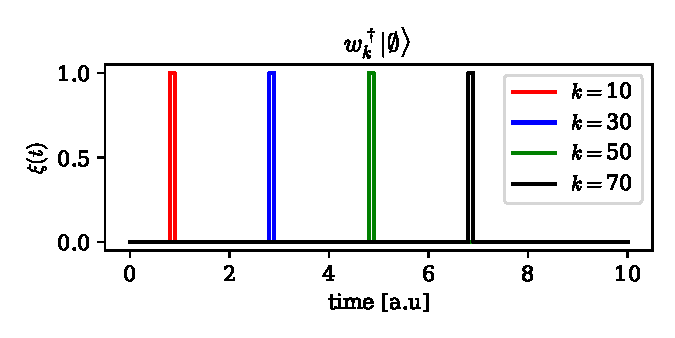
\includegraphics[width=0.6\linewidth]{figures/creationoperation.pdf}
    \caption{The one-photon wavefunction $\xi^{(1)}(t)$ as a function of time for the state $w_k^\dagger \ket{\emptyset} = \sum_i \xi(t_i) \ket{1_i}$ with $\xi(t_i) = \delta_{i,k}$ for different $k$'s. }
    \label{fig:creationoperator}
\end{figure}


Let us consider if we want to add two waveguide operators. If they were matrices, we could just add the elements together, but this is not possible with the LazyOperator implementation. Instead, we create another LazyOperator object \code{LazySum}, representing the sum of operators. The structure of the \code{LazySum} can be seen in 
Code Sample \ref{ls:lazysum}. Lines 1-6 define the structure, where \code{factors} are for arithmetic operations, and \code{operators} is a vector or tuple containing the operators to be summed. Lines 7-12 define how LazySum objects are added together; the fields \code{factors} and \code{operators} are concatenated, and a new LazySum object is instantiated. Lines 13-19 define the multiplication routine, where we loop over all operators in the \code{operators} field. Adding two waveguide operators can thus just be defined as creating a \code{LazySum} object as shown in Code Sample \ref{ls:additionwaveguide}.

\begin{listing}[H]
\begin{minted}[
frame=lines,
framesep=2mm,
baselinestretch=1.2,
bgcolor=LightGray,
fontsize=\small,
linenos,
escapeinside=||,
mathescape=true
]{julia}
mutable struct LazySum{BL,BR,F,T} <: AbstractOperator{BL,BR}
    basis_l::BL
    basis_r::BR
    factors::F
    operators::T
end
function +(a::LazySum{B1,B2}, b::LazySum{B1,B2}) where {B1,B2}
    check_samebases(a,b)
    factors = _cat(a.factors, b.factors)
    ops = _cat(a.operators, b.operators)
    @samebases LazySum(a.basis_l, a.basis_r, factors, ops)
end
function mul!(result::Ket{B1},a::LazySum{B1,B2},b::Ket{B2},alpha,beta) where {B1,B2}
    mul!(result,a.operators[1],b,alpha*a.factors[1],beta)
    for i=2:length(a.operators)
        mul!(result,a.operators[i],b,alpha*a.factors[i],1)
    end
    return result
end
\end{minted}
\caption{LazySum implementation. Lines 1-6 define the structure. Lines 7-12 define how LazySum objects are added together. Lines 13-19 define the multiplication operation.}
\label{ls:lazysum}
\end{listing}

\begin{listing}[H]
\begin{minted}[
frame=lines,
framesep=2mm,
baselinestretch=1.2,
bgcolor=LightGray,
fontsize=\small,
linenos,
escapeinside=||,
mathescape=true
]{julia}
function +(a::WaveguideOperator,b::WaveguideOperator)
    @assert a.basis_l == b.basis_l
    @assert a.basis_r == b.basis_r
    LazySum(a) + LazySum(b)
end
two_wd = wd + wd #LazySum
\end{minted}
\caption{Addition of waveguide operators returning a LazySum. }
\label{ls:additionwaveguide}
\end{listing}

In all of the above, we assumed that we were only considering the Hilbert space waveguide. However, we want to combine the waveguide operator with other quantum systems through the tensor product. Naturally, we, therefore, need to introduce a LazyTensor object. The code for performing the lazy tensor product is much more complicated than the lazy sum case. Thus, instead of going over the code in its entirety, we instead consider a specific example and illustrate how we can perform a lazy tensor operation. Let us consider a tensor product between two two-level systems. We can write this as:
\begin{equation}
    \left (a\ket{g}+b\ket{e} \right ) \otimes \left(c\ket{g}+d\ket{e} \right) =  \begin{pmatrix} {a} \\ {b} \end{pmatrix} \otimes \begin{pmatrix} {c} \\ {d} \end{pmatrix} = \begin{pmatrix} {a}{c} \\ {a} {d} \\ {b}{c} \\ {b}{d} \end{pmatrix}
\end{equation}
The transition operator for excited to ground state is $\sigma = \ket{g}\bra{e} = \begin{pmatrix}
    0 & 0 \\ 1 & 0
\end{pmatrix}$ and if we want to apply it to the second emitter, we tensor it with the identity operator. Without inferring the tensor product lazily, this would look like:
\begin{equation}
     I \otimes \sigma  \begin{pmatrix} {a}{c} \\ {a}{d} \\ {b}{c} \\ {b}{d} \end{pmatrix} =  \begin{pmatrix}
    1 & 0 \\ 0 & 1
\end{pmatrix} \otimes \begin{pmatrix}
    0 & 1 \\ 0 & 0
\end{pmatrix} \begin{pmatrix} {a}{c} \\ {a}{d} \\ {b}{c} \\ {b}{d} \end{pmatrix} = \begin{pmatrix}
0 & 1 & 0 & 0 \\
0 & 0 & 0 & 0 \\
0 & 0 & 0 & 1 \\
0 & 0 & 0 & 0
\end{pmatrix} \begin{pmatrix} {a}{c} \\ {a}{d} \\ {b}{c} \\ {b}{d} \end{pmatrix} = \begin{pmatrix} {a}{d} \\ 0 \\ bd \\ 0 \end{pmatrix}
\end{equation}

This operation could, however, also have been done by first applying $\sigma$ to the first two elements (notice we don't need to subsequently apply the identity operator):
\begin{equation}
    I \otimes \sigma \begin{pmatrix} {a}{c} \\ {a}{d} \\ {b}{c} \\ {b}{d} \end{pmatrix} = \begin{pmatrix}
    \color{red}{\begin{pmatrix}
    0 & 1 \\ 0 & 0
\end{pmatrix}} \\ \color{blue}{\begin{pmatrix}
    0 & 1 \\ 0 & 0
\end{pmatrix}}
\end{pmatrix} \begin{pmatrix} \color{red}{a}{c} \\ \color{red}{a}{d} \\ \color{blue}{b}{c} \\ \color{blue}{b}{d} \end{pmatrix} = \begin{pmatrix} \color{red}{a}{d} \\ 0 \\ \color{blue}{bd} \\ 0 \end{pmatrix}
\end{equation}
where it is here understood that the red matrix is applied to red elements and the blue matrix to blue elements. If we instead wanted to apply $\sigma \otimes I$, this would look like: 
\begin{equation}
    \sigma \otimes I \begin{pmatrix} {a}{c} \\ {a}{d} \\ {b}{c} \\ {b}{d} \end{pmatrix} = \begin{pmatrix}
    \color{red}{\begin{pmatrix}
    0 & 1 \\ 0 & 0
\end{pmatrix}} \\ \color{blue}{\begin{pmatrix}
    0 & 1 \\ 0 & 0
\end{pmatrix}}
\end{pmatrix} \begin{pmatrix} \color{red}{a}{c} \\ \color{blue}{a}{d} \\ \color{red}{b}{c} \\ \color{blue}{b}{d} \end{pmatrix} = \begin{pmatrix} \color{red}{b}{c} \\  \color{blue}{b}{d}  \\ 0 \\ 0 \end{pmatrix}
\end{equation}
We are now applying the matrices on a smaller vector formed by taking every second element. The formula for the index $\mathrm{I}$ of element $i$ in system 1 and element $j$ in system 2 is: $\mathrm{I} = i + 2\cdot(j-1)$. More generally, if we have multiple systems, we can access any arbitrary element by calculating the index as shown in Code Sample \ref{ls:lazy_index}:
\begin{listing}[H]
\begin{minted}[
frame=lines,
framesep=2mm,
baselinestretch=1.2,
bgcolor=LightGray,
fontsize=\small,
linenos,
escapeinside=||,
mathescape=true
]{julia}
I = indices[1]
for k in 2:length(indices)
    I += strides[k]*(indices[k]-1)
end
\end{minted}
\caption{Calculates the index \code{I} to access element \{i,j,k,...\} given by the vector \code{indices}. \code{Strides} is a vector containing strides for each sub-Hilbert space and is calculated in Code Sample \ref{ls:lazy_stride} }
\label{ls:lazy_index}
\end{listing}
where \code{indices} is a vector containing the indices of the elements that we want to access such that the first element $i$ is the index of the element in subsystem 1, the second element $j$ is the index of the element in subsystem 2, and so forth. \code{strides} is a vector containing the strides of the basis and can be calculated as shown in Code Sample \ref{ls:lazy_stride}:
\begin{listing}[H]
\begin{minted}[
frame=lines,
framesep=2mm,
baselinestretch=1.2,
bgcolor=LightGray,
fontsize=\small,
linenos,
escapeinside=||,
mathescape=true
]{julia}
strides[1] = 1
for m=2:length(shape)
    strides[m] = strides[m-1]*shape[m-1]
end
\end{minted}
\caption{Calculates the stride of each sub-Hilbert space, here \code{shape} is the sizes of the sub-Hilbert spaces. }
\label{ls:lazy_stride}
\end{listing}
where \code{shape} is the sizes of the subsystems. In the above case \code{shape = (2,2)} and \code{strides = (1,2)}. Using these indices, we can infer how the operators should be applied. The actual code for performing the LazyTensor product is a bit more involved but uses this principle. A Code Sample can be seen in appendix \ref{app:lazytensor}.

With the LazyOperators implemented, we are now ready to solve a two-photon pulse scattering on a cavity. In Fig.~\ref{fig:lazybench}, we benchmark the LazyOperator implementation vs. the Sparse operator implementation. The performance gain is huge for more than $\approx 50$ bins. Note that the time for the LazyOperator benchmark is both creating the operators and solving the problem. There is some small constant overhead related to creating the LazyOperators, which for small numbers of bins, makes it slightly slower than the sparse method. However, the time-bin picture is barely valid for this number of bins. In any realistic simulation, more than $100$ bins are used, and the performance gain is significant. The performance gain comes from not having to allocate the matrices and also because we are no longer looping through a sparse matrix where looking up indices is slow.     

\begin{figure}[H]
    \centering
    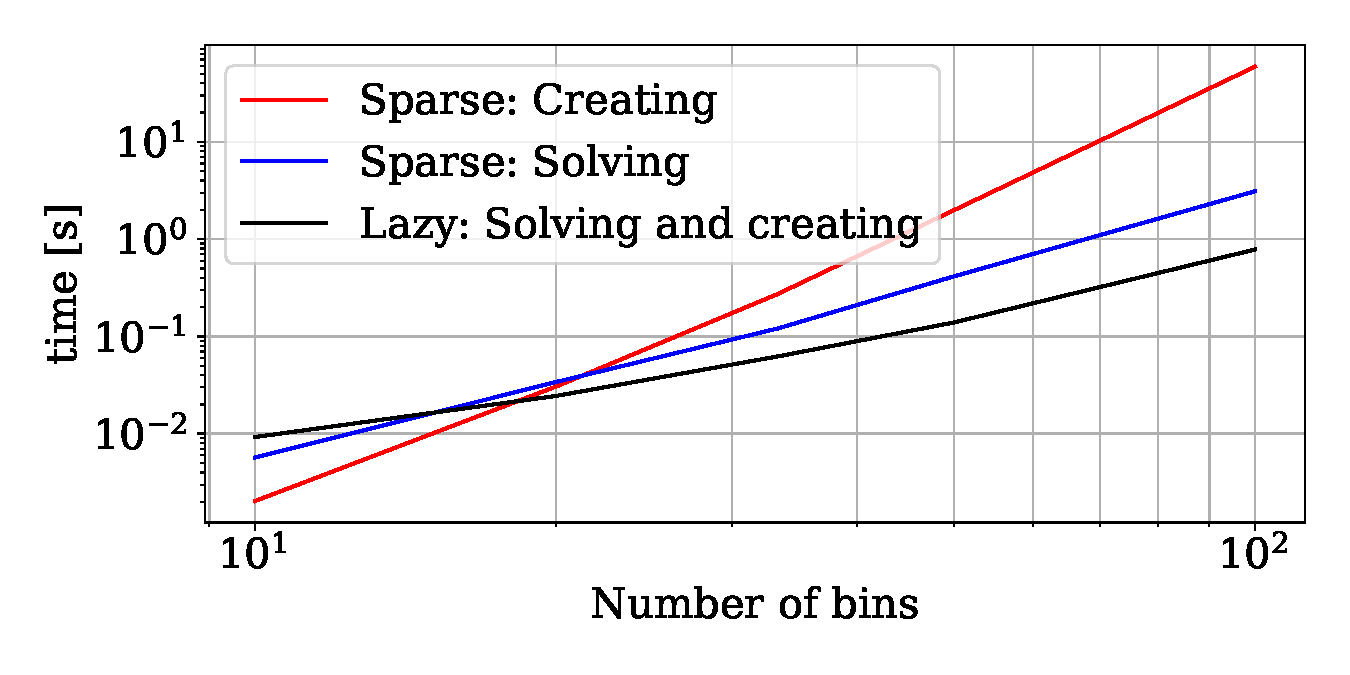
\includegraphics[width=0.6\linewidth]{figures/lazy_bench.pdf}
    \caption{Benchmark of lazy operator implementation compared to the time taken to create Hamiltonians in sparse version, and time taken to solve the problem in sparse version. We see that the time taken to solve the problems is almost equivalent, meaning that there is effectively no overhead in creating the Lazy operators.}
    \label{fig:lazybench}
\end{figure}


\section{Twophoton Scattering: Cavity vs. Emitter \label{sec:twophoton_emitter_vs_cavity}}
One of the major advantages of the numerical implementation in WaveguideQED.jl is flexibility. In this section, we will illustrate the flexibility by considering the scattering of a two-photon pulse on a cavity and emitter, respectively. In sec.~\ref{sec:twophoton_continuous}, we derived the equations of motion for a two-photon pulse scattering on a cavity, and we can use these to confirm that our implementation is also working for two-photon states. For the scattering of an emitter, even though it is mathematically close to the cavity (we just restrict the total number of photons to one), we would have to rederive the equations of motion as this introduces non-trivial effects, such as stimulated emission. In the numerical framework, it is trivial to change the operator $a \rightarrow \sigma$ thus showcasing its strength.


 We start by considering the scattering of a two-photon pulse in Fig.~\ref{fig:twophoton_detuning}. The code for setting this up in WaveguideQED.jl is shown in Code Sample \ref{ls:twophoton_scattering}, and a convergence study using the hierarchical differential equations in eq.~\eqref{eq:twophotonEOM} is done in appendix \ref{app:twophoton_convergence}. Note that the waveguide operators \code{w} and \code{wd} in Code Sample \ref{ls:twophoton_scattering} are effortlessly combined with operators from QuantumOptics.jl. Behind the scenes, lazy operations such as LazyTensor, LazySum, and LazyProduct, are all performed such that the user can manipulate the operators with $\otimes$,$+$,$-$, and $*$ as if they were standard operators defined via matrices. This allows for flexibility in setting up simulations and gives an intuitive user interface. 
 
 The initial state here consists of two one-photon Gaussian pulses $\ket{\psi}_{in} = \sum_k \sum_j \xi^{(2)}(t,t') \Delta t w_k^\dagger w_j^\dagger \ket{\emptyset}$ with $\xi^{(2)}(t,t') = \xi^{(1)}(t) \xi^{(1)}(t')$ and $\xi^{(1)}(t)$ given in \ref{eq:gaussian}. In the top row, we show the two-photon wavefunction $\xi^{(2)}(t,t')$, and in the lower row, we show the SVD one-photon wavefunctions $\lambda_i^2 \abs{\phi_i(t)}^2$ with the three largest singular values $\lambda_i$ (see eq.~\eqref{eq:SVD}). We find that in all cases, the largest singular value is one, meaning that the scattered two-photon state is still in a product state. Indeed, the wavefunctions in the scattered single-photon case shown in Fig.~\ref{fig:singlephoton_wf} are identical to SVD wavefunction $\phi(t)$ in the two-photon case. After the scattering, we thus just have a product state of the single-photon scattered wavefunctions and the photons have thus not really interacted with each other, but just scattered separately off the cavity. 


\begin{listing}[H]
\begin{minted}[
frame=lines,
framesep=2mm,
baselinestretch=1.2,
bgcolor=LightGray,
fontsize=\small,
linenos,
escapeinside=||,
mathescape=true
]{julia}
times  = 0:0.01:15
bc = FockBasis(2) #Change to 1 to simulate emitter.
bw = WaveguideBasis(2,times)
a = destroy(bc)
ad = create(bc)
w = destroy(bw)
wd = create(bw)
n = ad*a |$\otimes$| identityoperator(bw)
wda = a |$\otimes$| wd
adw = ad |$\otimes$| w
H = |$\delta$|*n + im*sqrt(|$\gamma$|/dt)*(adw-wda)

xi(t,s,t0) = sqrt(2/s)* (log(2)/pi)^(1/4)*exp(-2*log(2)*(t-t0)^2/s^2)
xi2(t1,t2,s1,s2,t0) = xi(t1,s1,t0)*xi(t2,s2,t0)
psi_waveguide = twophoton(bw,xi2,times,1,1,5)
psi_in = fockstate(bc,0) |$\otimes$| psi_waveguide

psi_out = waveguide_evolution(times, psi_in, H)
\end{minted}
\caption{Code for simulating the scattering of a two-photon pulse. Line 1-11 sets up the Hamiltonian, while 13-16 define the input state (\code{twophoton} takes in a function \code{xi2} defining the wavefunction and creates a two-photon state with this wavefunction). In line 18, we solve scattering with a differential equation solver.}
\label{ls:twophoton_scattering}
\end{listing}


If instead of the cavity, we consider a two-level system, stimulated emission triggered by the second photon leads to a strong correlation between the two photons: Observing the first means you are more likely to observe the second one. This is shown in Fig.~\ref{fig:twophoton_emitter_detuning}, where we consider the scattered wavefunction and the three most populated one-photon decompositions. The wings of the bird-like structure of the scattered wavefunction $\xi^{(2)}(t_1,t_2)$ for $\delta = 0$ correspond to an entanglement in time between the two photons. Similarly, it is evident that the single-photon decomposition requires multiple wavefunctions, and we thus no longer have a simple product state. Due to the saturation of the emitter, which can only be excited by one photon, the two photons thus effectively interact through the emitter, by stimulated emission. As the detuning increases, the pulse and the emitter interaction diminishes, and we recover a scattered product state (for $\delta = 5$, we have $\lambda_1^2 = 0.998$).

\

\begin{figure}
    \centering
    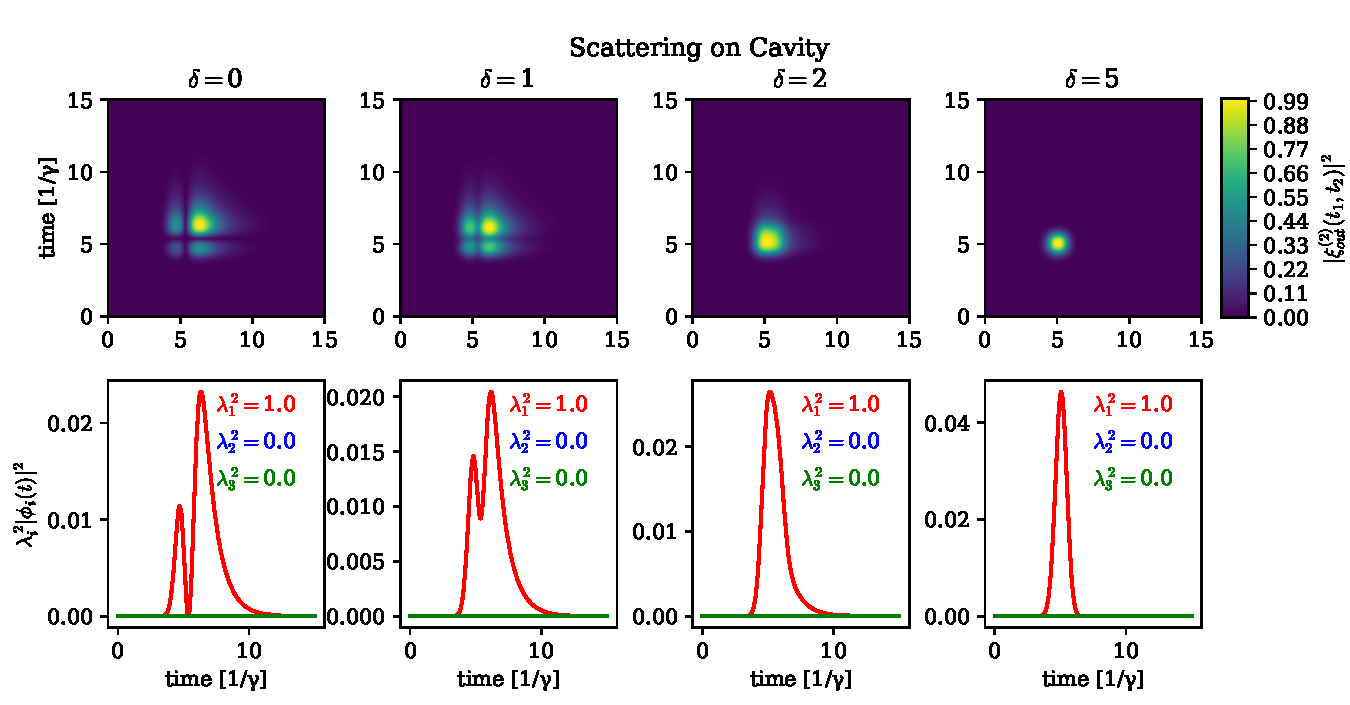
\includegraphics[width = 0.94\linewidth]{figures/twophoton_cavity_detuning.pdf}
    \caption{Scattering of a two-photon pulse on a single-sided cavity with a Gaussian product state $\ket{\psi}_{in} = \int dt \int dt' \xi_{in}^{(2)}(t,t') \ket{1_t}\ket{1_{t'}}$ where $ \xi_{in}^{(2)}(t,t') = \xi_{in}^{(1)}(t)\xi_{in}^{(1)}(t')$ with $\xi_{in}^{(1)}(t)$ given in eq.~\eqref{eq:gaussian} for different detunings $\delta$. Upper panels: The scattered two-photon state wavefunction $\xi_{out}^{(2)}(t,t')$ from the state $\ket{\psi}_{out} = \int dt \int dt' \xi_{out}^{(2)}(t,t') \ket{1_t}\ket{1_{t'}}$. All contour plots are normalized so that the largest value is unity. Lower panels: SVD (see eq.~\eqref{eq:SVD}) composition of the scattered two-photon state $\xi_{out}^{(2)}(t,t')$ with the three largest singular value functions shown. Noticeably only one SVD is relevant and the cavity thus also outputs a product state.} 
    \label{fig:twophoton_detuning}
\end{figure}



\begin{figure}
    \centering
    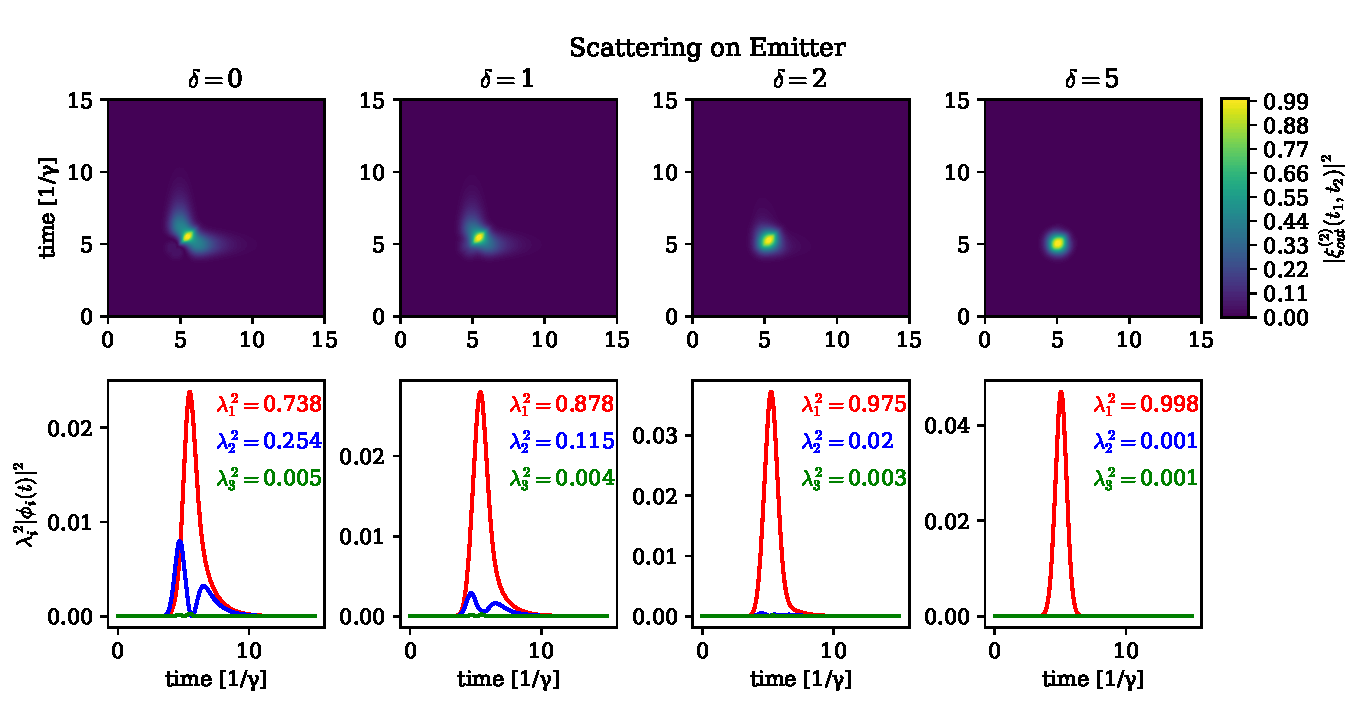
\includegraphics[width = 0.94\linewidth]{figures/twophoton_emitter_detuning.pdf}
    \caption{Same as Fig.~\ref{fig:twophoton_detuning} but scattering on a two-level system. The nonlinearity of the two-level-system gives an entangled two-photon state that can not be decomposed into a single function, which is seen in the SVD. }
    \label{fig:twophoton_emitter_detuning}
\end{figure}

\chapter{Multiple waveguides}
This chapter introduces how to model interactions with multiple waveguides (or equivalently multiple waveguide modes) in the time-binned photon picture. We will show how this can be used to extend the simulations in chapter \ref{ch3} so that we are no longer restricted to only one propagating mode. We consider an emitter coupled to two directional waveguide modes and reproduce results from a recent experimental demonstration of two-photon scattering in photonic crystal waveguides \cite{LeJeannic2022DynamicalEmitter}. We also consider how to model direct interactions between waveguide modes. Such interactions can arise from scattering elements in the waveguide leading to, e.g., a beamsplitter. We start by considering a fundamental Hamiltonian shown to obey flux conservation and time-reversal symmetry as required by input-output theory or in the classical limit: coupled mode theory. By discretizing the Hamiltonian into time bins, we find a discrepancy between the expected input-output relations and the discretized Hamiltonian. We investigate this discrepancy by considering the change in the lifetime of an emitter coupled to a waveguide with a scattering element. We find inconsistencies in the emitter lifetime found by the numerical approach but also show that these can be solved by an effective renormalization of the interaction strength between the emitter and waveguide modes. 
\begin{figure}[H]
    \centering
    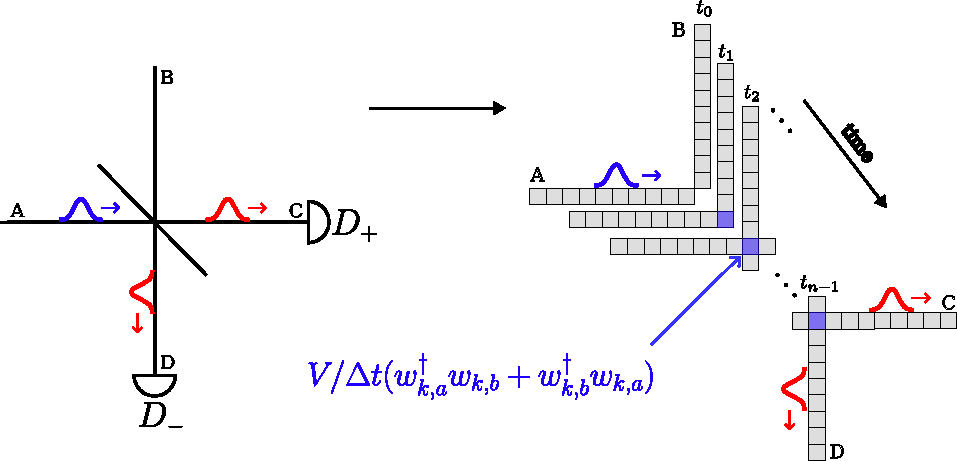
\includegraphics[width = \linewidth]{figures/waveguideinteraciton.pdf}
    \caption{Left: Sketch of a beamsplitter, where an incoming pulse (blue) scatters on the beamsplitter and is split into two identical output pulses (red). Right: Numerical representation of the interaction between binned photons in two waveguides. The initial state is defined at $t_0$, and when $t_n$ is reached, the two pulses have interacted, and in the shown sketch, the beamsplitter transformation has been performed. }
    \label{fig:beamsplitter_illustration}
\end{figure}


\section{Representing multiple waveguides efficiently }

Before we simulate the interactions with multiple waveguides, we will discuss how to represent them numerically. The naive approach is to define two waveguide bases, as introduced in chapter \ref{ch3}, and do a tensor product between them. However, a quick estimate of the total size of the Hilbert space reveals this approach to be infeasible. Suppose we want to describe two waveguide modes interfering on a beam splitter. Although the initial state only contains a single photon in each waveguide, we can have two photons in the waveguides after the interaction. Thus, we need two waveguide bases for modes $a$ and $b$, each containing up to two photons. If we take $N=100$, we thus have two Hilbert spaces each of size: $1+N+N(N+1)/2 = 5151$, meaning a combined Hilbert space of size: $5151^2 = 26,532,801$!!! Even with the LazyOperators and sparse representations, this is too large to be numerically feasible. Luckily, we can create a much more efficient storing strategy by realizing that we are storing unnecessary parts of the state vector. In this example, we only have a total of two excitations, meaning that states with two photons in each waveguide simultaneously are unobtainable, that is, states of the type: $\sum_{i,j,k,l}\xi^{(4)}(t_i,t_j,t_k,t_j) \ket{1_i,1_j}_a\ket{1_k,1_j}_b$, where the subscripts $a$ and $b$ denote waveguide modes $a$ and $b$, respectively. Therefore, if we restrict ourselves to states only containing at max two excitations, the Hilbert space reduces drastically in size. We are thus describing states with the general form:
\begin{align}
    \ket{\psi} &= \ket{\emptyset}_a\ket{\emptyset}_b + \sum_k \xi_a^{(1)}(t_k) \ket{1_k}_a\ket{\emptyset}_b + \sum_k \xi_b^{(1)}(t_k) \ket{\emptyset}_a\ket{1_k}_b + \sum_{k,l \geq k}\xi_a^{(2)}(t_k,t_j) \ket{1_k,1_j}_a \ket{\emptyset}_b \\ 
    &+ \sum_{k,l \geq k}\xi_b^{(2)}(t_k,t_j) \ket{\emptyset}_a \ket{1_k,1_j}_b+ \sum_{k,l}\xi_{a,b}^{(2)}(t_k,t_j) \ket{1_k}_a \ket{1_j}_b
\end{align}

\begin{figure}
    \centering
    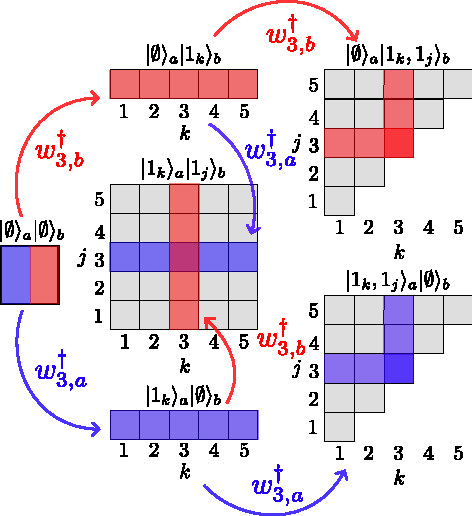
\includegraphics[width = 0.6 \linewidth]{figures/multiplewaveguides_illustration.pdf}
    \caption{Illustration of numerical representation of two waveguides containing two excitations. Blue colors are associated with creating a photon in waveguide $a$ and red with creating a photon in $b$. }
    \label{fig:twowaveguide_illustration}
\end{figure}

Notice that we now have a new two-time wavefunction $\xi^{(2)}_{a,b}(t_k,t_j)$ describing having a single-photon excitation simultaneously in waveguide $a$ and $b$. $\xi^{(2)}_{a,b}(t_k,t_j) = \xi^{(2)}_{a,b}(t_j,t_k)$ is in general not true, and we thus store a $N^2$ matrix to represent this state. An illustration of the total state of two waveguides containing two excitations can also be seen in Fig.~\ref{fig:twowaveguide_illustration}. Here, we also show the effect of acting with the creation operators $w^\dagger_{3,a/b}$, where all blue lines are associated with creating a photon in waveguide mode $a$ and red lines with creating photons in waveguide mode $b$. Our Hilbert space is now of size $1+N+2 N(N+1)/2 + N^2 = 20201$, thus three orders of magnitude smaller than the initial naive approach!

\

If we had more than two waveguides, we would need to store a combination of one photon in one waveguide and one photon in another. Considering three waveguide modes $a$, $b$, and $c$, we would thus have the following combinations $\ket{1_i}_a\ket{1_j}_b$, $\ket{1_i}_b\ket{1_j}_c$, and $\ket{1_i}_a\ket{1_j}_c$ (as well as two photons in the same waveguide $\ket{1_i,1_j}_{a}$, $\ket{1_i,1_j}_{b}$, and $\ket{1_i,1_j}_{c}$). When creating a waveguide basis with three waveguides using \code{bw = WaveguideBasis(Np,Nw,times)}, all of these combinatorics are done automatically. Here, \code{Np} is the number of photons in total, and $\mathrm{Nw}=3$ is the number of waveguide modes. Addressing the individual waveguides is likewise done by indexing the waveguide operator: \code{w = destroy(bw,i)}, where \code{i}, here is indexing the i'th waveguide mode in the basis. With this interface, we can easily consider multiple waveguide modes effortlessly, and we showcase this in the following section.  





\section{Scattering On a Single Emitter \label{sec:lodahl}}
\begin{figure}[H]
    \centering
    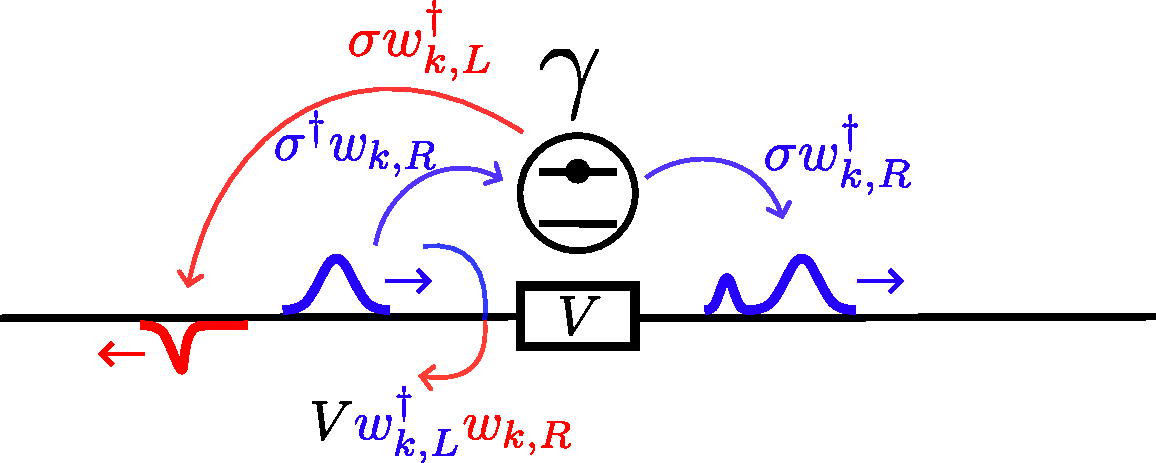
\includegraphics[width=\linewidth]{figures/lodahl_waveguide.pdf}
    \caption{Illustration of a right propagating excitation (blue) in a waveguide coupled to a two-level system with the factor $\gamma$. After the blue pulse has scattered, there is also an excitation going to the left (red). A coupling between the left and right propagating modes $V$ is also shown, which can be thought of as a partially transmitting mirror in the waveguide.}
    \label{fig:lodahl_sketch}
\end{figure}

With an effective representation of multiple waveguides, we can now simulate an emitter coupled to multiple waveguide modes. In Fig~\ref{fig:lodahl_sketch}, we show a waveguide with two directionally propagating modes (left and right) coupled to a two-level system with the rate $\gamma$. In the waveguide, we have also placed a partially transmitting mirror (PTE) which couples the left and right propagating modes with each other with a strength $V$. We will discuss this PTE and how to model it in detail in later sections. We start by considering the scattering element to be completely transparent, and the Hamiltonian for this configuration is:
\begin{equation}
    H_k = \sqrt{\gamma_\mathrm{L}/\Delta t} ( \sigma^\dagger w_{k,\mathrm{L}} + \sigma w^\dagger_{k,\mathrm{L}} ) + \sqrt{\gamma_\mathrm{R}/\Delta t} ( \sigma^\dagger w_{k,\mathrm{R}} + \sigma w^\dagger_{k,\mathrm{R}})  \label{eq:lodahl_ham}
\end{equation}
Here, we have introduced subscripts $\mathrm{R}$ and $\mathrm{L}$ to denote right and left propagating excitations. $\gamma_i$ denotes the coupling to waveguide $i$, which we assume in the following to be symmetric $\gamma_R = \gamma_L = \gamma/2$. This system is studied theoretically in ref. \cite{Joanesarson2020Few-photonGeometries} and experimentally in ref. \cite{LeJeannic2022DynamicalEmitter}, where a quantum dot is placed in a photonic crystal waveguide.
\begin{listing}[H]
\begin{minted}[
frame=lines,
framesep=2mm,
baselinestretch=1.2,
bgcolor=LightGray,
fontsize=\small,
linenos,
escapeinside=||,
mathescape=true
]{julia}
#Define basis
times = 0:0.1:10
be = FockBasis(1)
bw = WaveguideBasis(2,2,times)

#Define operators for interacting with emitter
swdR = create(bw,1) |$\otimes$| destroy(be)
sdwR = destroy(bw,1) |$\otimes$| create(be)
swdL = create(bw,2) |$\otimes$| destroy(be)
sdwL = destroy(bw,2) |$\otimes$| create(be)

#Setup Hamiltonian
|$\gamma R$|,|$\gamma L$| = 1,1
H = im*sqrt(|$\gamma R$|/dt)*(sdwL-swdL) + im*sqrt(|$\gamma R$|/dt)*(sdwR-swdR)

#Initial state
w=1 #width of gaussian pulse
psi_in_two = twophoton(bw,1,xi2,w,w,t0) |$\otimes$| fockstate(be,0)
psi_in_single = onephoton(bw,1,xi,w,t0) |$\otimes$| fockstate(be,0)
\end{minted}
\caption{Code for simulating scattering of emitter coupled to two channels. In lines 1-3, we define the bases used. Lines 7-10 define $\sigma w^\dagger_{k,\mathrm{R}/\mathrm{L}}$, and lines 13-14 combine the operators to define the Hamiltonian. In line 18, we define the initial two-photon state, and in line 19 the single-photon state. \code{xi} and \code{xi2} are Gaussian functions as also defined in Code Sample \ref{ls:twophoton_scattering} and studied in Fig.~\ref{fig:twophoton_detuning} and \ref{fig:twophoton_emitter_detuning}. }
\label{ls:lodahlcode}
\end{listing}

In the following, we show that with the Hamiltonian in eq.~\eqref{eq:lodahl_ham}, we can reproduce the results of the experiment in ref. \cite{LeJeannic2022DynamicalEmitter}, where the difference between scattering a two-photon pulse or a one-photon pulse on an emitter in a waveguide is considered. In Code Sample \ref{ls:lodahlcode}, we define the system's Hamiltonian and the initial state in the WaveguideQED.jl framework. We see that extending to multiple waveguides amounts to creating a waveguide-basis with two waveguides \code{WaveguideBasis(2,2,times)} and addressing the different modes in the basis is just indexing the waveguide operators by, for example, $w^\dagger_R = $\code{create(bw,1)}.
We also define two initial states; a single-photon Gaussian pulse and a two-photon Gaussian pulse, as studied previously in chapter \ref{ch3}. In Fig.~\ref{fig:lodahlfig2}, we vary the pulse width $\sigma$ and plot the transmitted two-photon wavefunction $\xi_{\mathrm{tt}}^{(2)}(t_1,t_2)$, where the subscripts $t$ here denotes that both photons are propagating in a transmitted state. For the two-photon state, this is the right propagating state after the interaction: $\xi_{\mathrm{tt}}^{(2)}(t_1,t_2) = \xi_{\mathrm{RR}}^{(2)}(t_1,t_2)$. In ref. \cite{LeJeannic2022DynamicalEmitter}, the scattered two-photon wavefunction is shown to factorize as $\xi_{\mathrm{RR}}^{(2)}(t_1,t_2) = \xi_\mathrm{R}^{(1)}(t_1)\xi_\mathrm{R}^{(1)}(t_2) + N(t_1,t_2)$, where $\xi_\mathrm{R}^{(1)}(t_1)$ denotes the single-photon scattered wavefunction and $N(t_1,t_2)$ describes the non-linear interaction between the two-photon pulse and the emitter. We can thus characterize the effect of this non-linearity by considering the single-photon product state 
 $\xi_{\mathrm{tt}}^{(2)}(t_1,t_2) = \xi_\mathrm{R}^{(1)}(t_1)\xi_\mathrm{R}^{(1)}(t_2)$ corresponding to measuring correlations between two separate single-photon pulses. 



In Fig~\ref{fig:lodahlfig2}, the single-photon product state and two-photon wavefunction are seen to be similar for narrow pulses. The emitter is unable to interact with the pulse effectively due to its short duration, and no appreciative non-linearity arises. As the width increases, a distinct difference, however, emerges. Similar to the scattering of the cavity, destructive interference leads to a reflection of the single-photon pulse, thus leading to a cross-like structure. For the two-photon pulse, we, however, have stimulated emission, which initially leads to a bird-like structure. For an even larger width $\sigma = 10/\gamma$, the diagonal shape indicates that the two photons arrive almost exclusively as a pair, showing a strong temporal correlation due to stimulated emission. 

\begin{figure}[H]
    \centering
    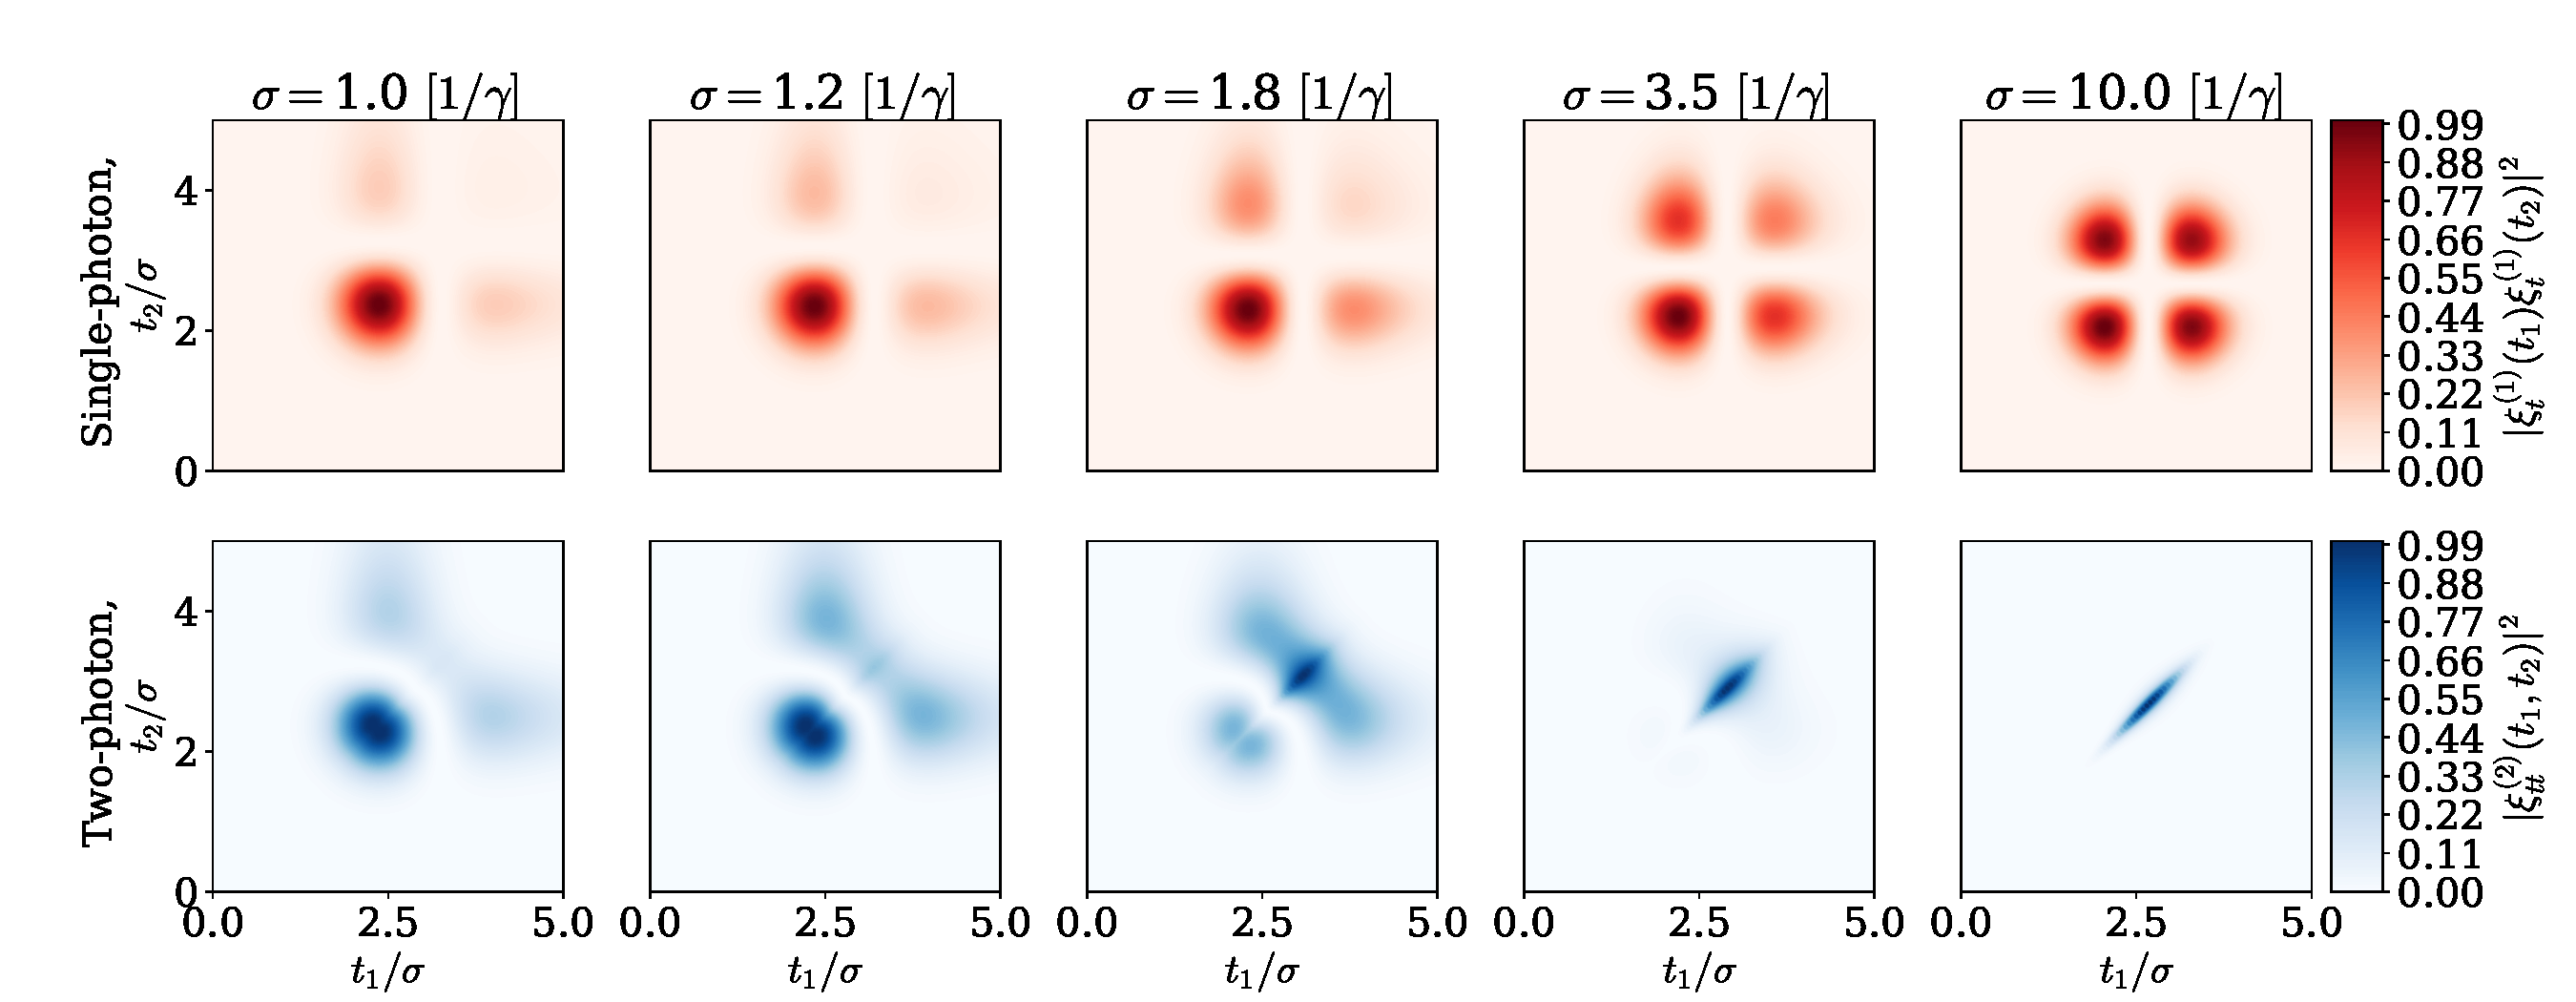
\includegraphics[width=\linewidth]{figures/lodahl_fig2.pdf}
    \caption{Upper panel (red): The product of two transmitted one-photon wavefunctions $|\xi_t^{(1)}(t_1)\xi_t^{(1)}(t_2)|^2$ from a single-photon Gaussian input state for varying widths of the Gaussian pulse $\sigma$. Lower panel (blue): Same as the upper panel but for a two-photon Gaussian input state. For ease of comparison, all contour plots have been normalized by dividing with largest value: $\mathrm{max}(|\xi_t^{(1)}(t_1)\xi_t^{(1)}(t_2)|^2)$ and $\mathrm{max}(|\xi_{tt}^{(2)}(t_1,t_2)$, respectively. \label{fig:lodahlfig2}}
\end{figure}

So far, this is all qualitatively very similar to the scattering of the emitter in the single-sided case. However, a clear distinction is seen if we consider not only the transmitted wavefunction but also the reflected wavefunction $\xi^{(2)}_{rr}$ (thus occupying the left propagating mode after the scattering) and partially reflected partially transmitted wavefunction $\xi^{(2)}_{rt}$. Here, $\xi^{(2)}_{rt}$ describes the amplitude of one photon in the reflected mode and one photon in the transmitted mode $\ket{1_i}_r\ket{1_j}_t$. In Fig.~\ref{fig:lodahlfig3}, we show these three scattered wavefunctions for a single-photon and two-photon Gaussian pulse for a width $\sigma = 1$. In the two-photon case, the reflected wavefunction $\xi^{(2)}_{rr}$ shows a dip along the diagonal, showing that two photons cannot be reflected simultaneously. This is exactly the opposite case of the transmitted wavefunction, where stimulated emission leads to simultaneous photon emission and, thus, a strong diagonal.

In the single-photon pulse, there is no dip in the diagonal as the separate pulses are both able to be reflected. As for the two-photon partially reflected, partially transmitted wavefunction, we see a highly asymmetric wavefunction, showing the time-ordering of the process: We will not see a photon in the reflected channel if we did not first observe a photon in the transmitted channel. For the single-photon pulse, no such restriction occurs because we are here comparing two separate pulses.




\begin{figure}[H]
    \centering
    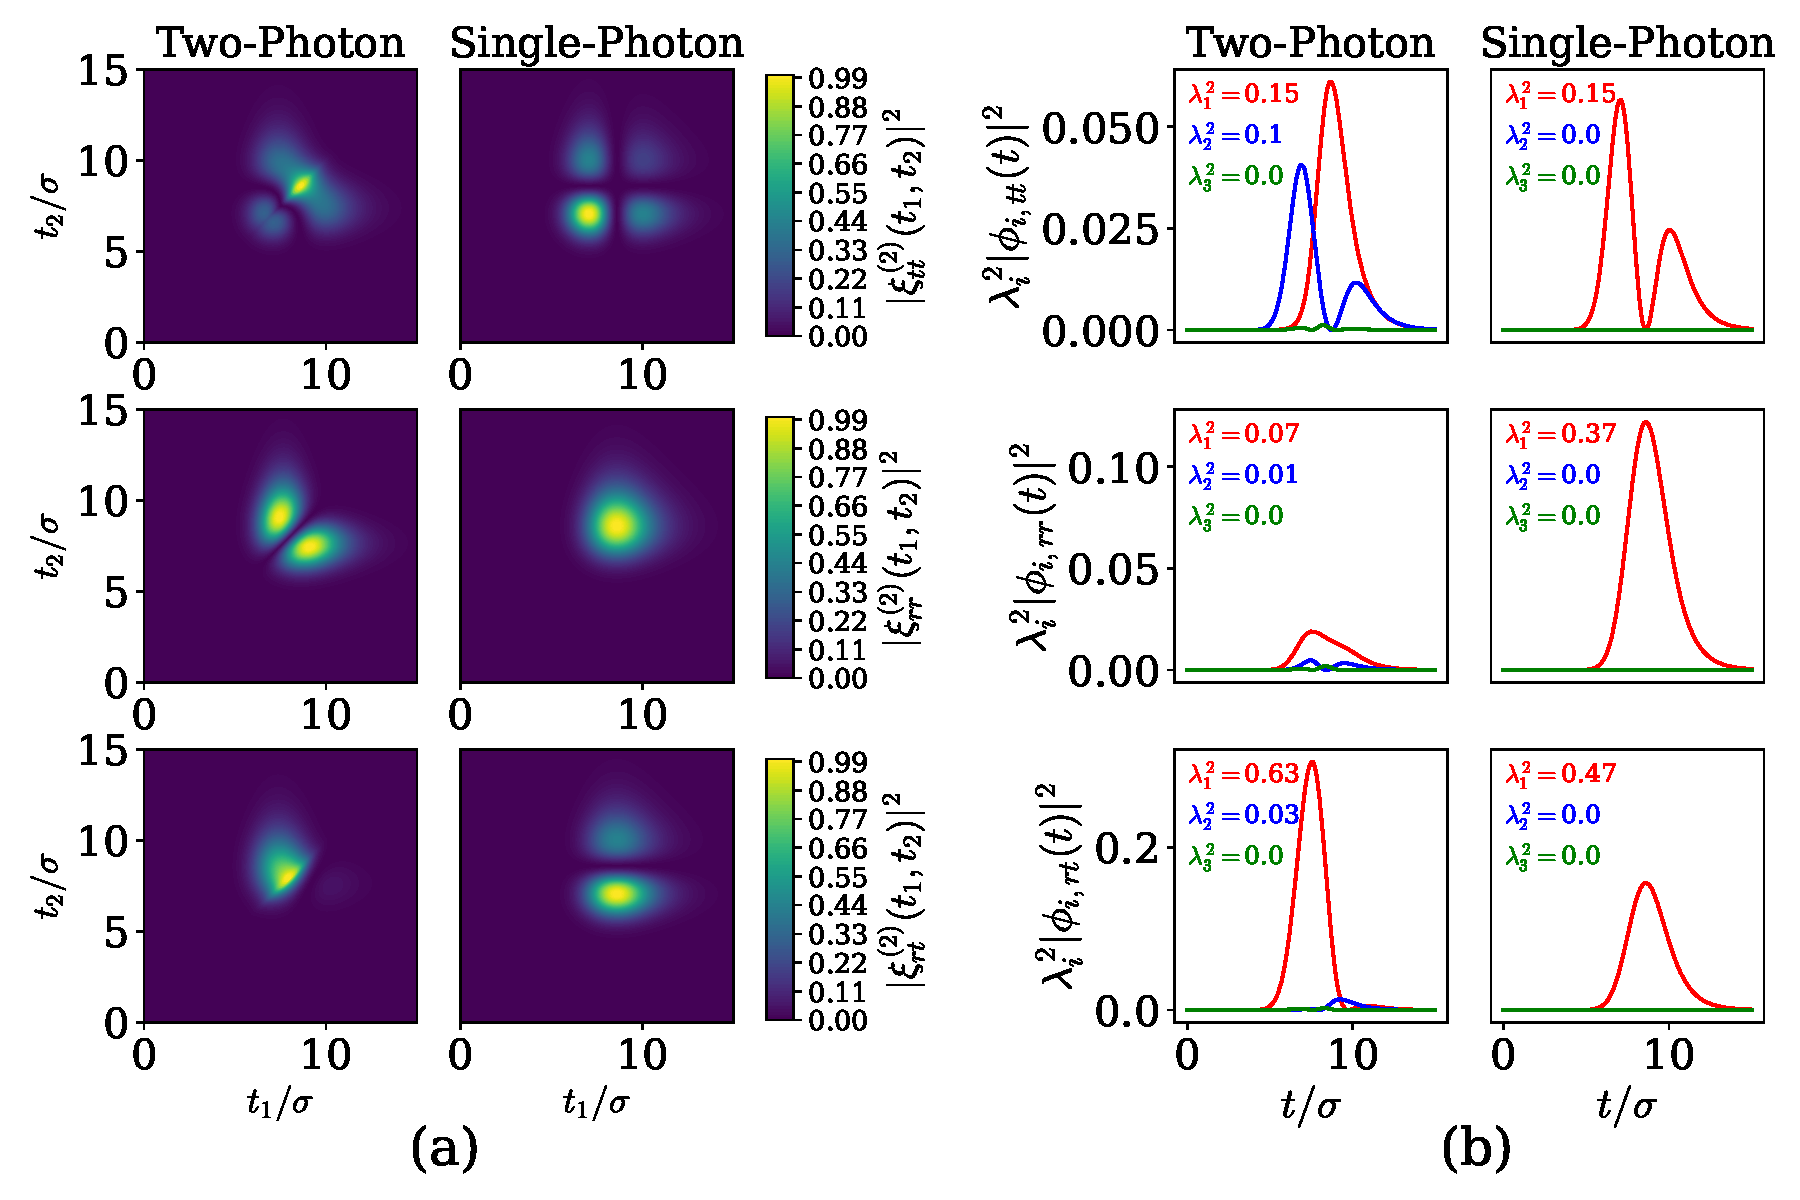
\includegraphics[width=\linewidth]{figures/lodahl_fig3.pdf}
    \caption{(a) Two-photon wavefunctions $\xi^{(2)}_{ij}(t_1,t_2)$ for width $\sigma = 2/\gamma$ with $\{i,j\} \in \{t,r\}$ describing the wavefunction of both photons being reflected, being transmitted, and one photon being reflected one photon being transmitted, respectively. The left column shows the scattered two-photon wavefunction, while the right shows the single-photon product state $\xi^{(2)}_{ij}(t_1,t_2) = \xi^{(1)}_{i}(t_1)\xi^{(1)}_{j}(t_2)$. All contour plots have been normalized so that the largest value corresponds to unity. (b) The three highest populated modes $\phi(t)$ of the decomposed two-photon wavefunctions. Obviously, the single-photon product state only has one populated decomposed mode $\phi(t)$.}
    \label{fig:lodahlfig3}
\end{figure}

In Fig.~\ref{fig:lodahlfig3}, we show the SVD of the wavefunctions and the occupation of the respective decomposed wavefunctions $\phi$. Note that the singular values $\lambda_i^2$ denote the weight of the decomposed function of the total scattered state. Thus $\sum_{i,\mu} \lambda_{i,\mu}^2 = 1$, where $\mu \in \{tt,rr,rt\}$ is the index of the transmitted-transmitted, reflected-reflected, reflected-transmitted state. The single-photon pulse is, by definition, only composed of a single product state, and thus only one relevant orthonormal wavefunction $\phi$ shows up for each scattered wavefunction. For the two-photon case, we see several relevant orthonormal wavefunctions similar to what was seen in ch.~\ref{ch3}. The evidence of stimulated emission is seen clearly, as the total population of the two photons being reflected is  significantly reduced with a population of approximately $0.08$ in the two-photon case vs. $0.37$ in the single-photon case, respectively. Similarly, there is an increase in both photons being transmitted with $0.1+0.15 = 0.25$ vs. $0.15$. Also, due to emitter saturation, we see an increase in the first photon being reflected and the second transmitted with $0.66$ vs. $0.48$.



\section{Input Output Relations \label{sec:inputoutput}}
If we now want to consider how waveguide modes can interact directly to form, for example, a partially transmitting element, we now need to define how they interact with each other. In ref. \cite{Xu2016FanoTransport}, they show that fundamental input-output relations can be derived from the Hamiltonian:
\begin{equation}
\begin{aligned}
H= H_{\mathrm{s}}+ \sum_{i=1}^N \int d \nu \hbar \nu w_{i}^{\dagger}(\nu) w_{i}(\nu)+\sum_{i=1}^N \hbar \sqrt{\gamma_i} \int \frac{d \nu}{\sqrt{2 \pi}}\left(w_{i}^{\dagger}(\nu) a+a^{\dagger} w_{i}(\nu)\right) +\sum_{i \neq j} \hbar V_{i j} \int \frac{d \nu}{\sqrt{2 \pi}} \int \frac{d  \nu^{\prime}}{\sqrt{2 \pi}} w_{i}^{\dagger}(\nu) w_{j}(\nu^\prime), \label{eq:generalFAN}
\end{aligned}
\end{equation}
where $w_{i}(\nu)$ is the annihilation operator for waveguide mode $i$ with frequency $\nu$, $\gamma_i$ is the coupling between a local system with Hamiltonian $H_s$ and waveguide mode $i$, and $V_{i,j} =V_{j,i}$ is the unitless coupling between waveguide modes (notice how $d \nu d\nu^\prime w_{i}^{\dagger}(\nu) w_{j}(\nu^\prime)$ has units of inverse time). $N$ is here the total number of waveguide modes. The input-output relations are here given as \cite{Xu2016FanoTransport}:
\begin{equation}
\begin{gathered}
\frac{d}{d t} a=-i\left[a, H_{\mathrm{c}}\right]-\Sigma a+\mathbf{k}^T \mathbf{W}_{\mathrm{in}} \\
\mathbf{W}_{\text {out }}(t)=\mathbf{C} \mathbf{W}_{\mathrm{in}}(t)+a(t)\mathbf{d}
\end{gathered}
\end{equation}
where 
\begin{equation}
    \mathbf{W}_{in} = \begin{pmatrix}
    w_{in,1}(t) \\ w_{in,2}(t) \\ \vdots \\ w_{in,N}(t)
\end{pmatrix}, \ \ \ \ \ \ \ \ \mathbf{W}_{out} = \begin{pmatrix}
   w_{out,1}(t) \\ w_{out,2}(t) \\ \vdots \\ w_{out,N}(t)
\end{pmatrix}    
\end{equation}
are vectors of the input waveguide operators before having interacted with the system and after having interacted, respectively. $\Sigma$ describes a self-energy correction due to the interaction with the waveguides, and $\mathbf{k}=\mathbf{d}$ is the effective coupling between the waveguides and quantum system. $\mathbf{C}$ describes the direct coupling between the waveguides. Indeed, if we had no coupling with the quantum system, the output field would just be $\mathbf{W}_{\text {out }}=\mathbf{C} \mathbf{W}_{\mathrm{in}}$. All of these relations can be defined in terms of the coupling between the waveguides $\mathbf{V}$ and between the waveguides and quantum system $\mathbf{\Gamma}$
\begin{equation}
\textbf{V} = \begin{pmatrix}
    0 & V_{1,2} & \cdots & V_{1,N} \\
    V_{2,1} & 0 & \cdots & V_{2,N} \\
     \vdots & \vdots & \ddots & \vdots \\
     V_{N,1} & V_{N,2} & \cdots & 0 \\
\end{pmatrix},   \ \ \ \ \ \ \ \ \ \ \mathbf{\Gamma} =  \begin{pmatrix}
     \gamma_1 \\
    \gamma_2 \\
    \vdots \\
    \gamma_N
\end{pmatrix}
\end{equation}
as:
\begin{equation}
\mathbf{C} \equiv\left(\mathbf{I}-\frac{i}{2} \mathbf{V}\right)\left(\mathbf{I}+\frac{i}{2} \mathbf{V}\right)^{-1}, \quad \mathbf{d} = \mathbf{k} \equiv-i\left(\mathbf{I}+\frac{i}{2} \mathbf{V}\right)^{-1} \mathbf{\Gamma}, \quad \Sigma \equiv \frac{1}{2} \mathbf{\Gamma}^T\left(\mathbf{I}+\frac{i}{2} \mathbf{V}\right)^{-1} \mathbf{\Gamma} \label{eq:coupling_definitions}
\end{equation}
From this, it is evident that the coupling with the system $\mathbf{k}=\mathbf{d}$ is not independent of the waveguide coupling $\mathbf{V}$. As we shall see, this can be interpreted as the waveguide coupling $\mathbf{V}$ altering the local density of optical states and thus changing the coupling between the waveguides and local system. 

 The input-output relations are defined in the Heisenberg picture, and describe how the operators transform under the interaction. The equivalent in the Schrodinger picture (and thus later on time-bin picture) is that the input state transforms as (for simplicity we consider a single-photon input state):
\begin{equation}
    \ket{\psi}_{in} = \sum_i \int dt' \xi_{in,i}(t') w_i^\dagger(t') \ket{\emptyset} \rightarrow \ket{\psi}_{out} = \sum_i \int dt' \xi_{out,i}(t') w_i^\dagger(t') \ket{\emptyset}
\end{equation}
with $\xi_{out,i}(t) = \sum_j C_{i,j} \xi_{in,j}(t) + d_i \psi_C(t)$ where $\psi_C(t)$ is the amplitude of the cavity.

As we will see, we cannot simply adopt the Hamiltonian in eq.~\eqref{eq:generalFAN} to the time-bin picture. In collision models, which the framework is based on, the baths (which, in this case, is the waveguide) are not allowed to interact internally. We will later solve this by an effective renormalization, and this is discussed in sec.~\ref{sec:inferringwaveguide}. For now, it is still instructive to consider the Hamiltonian in eq.~\eqref{eq:generalFAN} and transform it into the time-bin picture to see where the model breaks down. As it turns out, we can get the correct results if we do not consider coupling to another quantum system. When another quantum system is introduced, the renormalization of the coupling with the system is, however, not captured correctly. As shown in app~.\ref{app:rotating}, transforming the Hamiltonian in eq.~\eqref{eq:generalFAN} into the time-bin picutre leads to the Hamiltonian $H_k$ for time-bin $k$:
\begin{equation}
    H_{k} = H_{\mathrm{s}}- \hbar \omega_s a^\dagger a  + \sum_{i=1}^N \hbar \sqrt{\gamma_i/\Delta t} \left(w_{k,i}^{\dagger} a+a^{\dagger} w_{k,i} \right) + \sum_{i \neq j} \hbar  V_{i j}/\Delta t w_{k,i}^{\dagger} w_{k,j} \label{eq:general_transformed}
\end{equation}
where $\omega_s$ is the frequency around which the waveguide pulses are centered. Note, however, that in deriving the above time-bin Hamiltonian, we approximated:
\begin{equation}
   \int_{t_{n-1}}^{t_n} dt' w_i^\dagger(t') w_j(t') \approx \frac{1}{\sqrt{\Delta t}} \int_{t_{n-1}}^{t_n} d t' w^\dagger_{i}(t') \frac{1}{\sqrt{\Delta t}} \int_{t_{n-1}}^{t_n} d t' w_{j}(t') =  w^\dagger_{i,n} w_{j,n} \label{eq:interaction_ansatz}
\end{equation}
which is not obvious whether is true and likely is the source of failure, as we shall see later. Conceptually, it corresponds to having the two waveguides interacting only at a single point in space and, therefore, also in time. This is also illustrated in Fig.~\ref{fig:beamsplitter_illustration}, where two waveguides interact and form a beamsplitter. In the following, we thus consider no local system ($H_s = 0$) with two waveguide modes $a$ and $b$ (see app.~\ref{app:waveguideinteraction} for a derivation of the general case), and the Hamiltonian is:
\begin{equation}
    H_{k,\mathrm{int}} = \hbar V/\Delta t (w_{k,\mathrm{b}}^\dagger w_{k,\mathrm{a}} + w_{k,\mathrm{a}}^\dagger w_{k,\mathrm{b}})
    \label{eq:waveguideinteraction}
\end{equation}
where $w_{k, \mathrm{a} / \mathrm{b}}$ here is the waveguide operator of waveguide mode $a$ or $b$ at time-bin $k$, and $V$ is the interaction between waveguide modes $a$ and $b$. 
%After each time-bin has interacted, we thus have the state in the arms after the beamsplitter (here labeled c and d). As we shall see, the strength of $V$ decides the operation of the beamsplitter considered, i.e., whether it is balanced, unbalanced, applies a phase shift, etc.  

The input-output relations for the above interaction can be derived by considering how the operator at time-bin $k$ evolves. Since the Hamiltonian is constant within each time-bin and since we are only interacting with one time-bin at a time, we can write the time-evolution operator for time-bin $k$ as:
\begin{equation}
    U(t_k,t_k+\Delta t) =\exp \left[-\frac{i}{\hbar} \int_{t_k}^{t_k+\Delta t} H_{k,\mathrm{int}} d t^{\prime}\right] = \exp(- i V(w_{k,\mathrm{b}}^\dagger w_{k,\mathrm{a}} + w_{k,\mathrm{a}}^\dagger w_{k,\mathrm{b}} ))
\end{equation}

In the Heisenberg picture, we will thus have the following transformation after the interaction (see appendix \ref{app:waveguideinteraction}):
\begin{equation}
w_{k,\mathrm{a}}(t_k + \Delta t) = U^\dagger(t_k,t_k+\Delta t) w_{k,\mathrm{a}} U(t_k,t_k+\Delta t) = \cos(V) w_{k,\mathrm{a}} - i \sin(V) w_{k,\mathrm{b}}
\end{equation}
Similarly, we have:
\begin{equation}
w_{k,\mathrm{b}}(t_k + \Delta t) = \cos(V) w_{k,\mathrm{b}} - i \sin(V) w_{k,\mathrm{a}}
\end{equation}
This is exactly the beamsplitter transformation \cite{Gerry2004IntroductoryOptics}, and we see that for a 50:50 beamsplitter, we should choose $V_{a,b} = \pi/4$.  The coupling matrix $\mathbf{C}$ can thus be expressed as:
\begin{equation}
    \mathbf{C} = \begin{pmatrix}
        \cos(V) & -i \sin(V) \\
        -i \sin(V) & \cos(V)
    \end{pmatrix} \label{eq:C_timebin}
\end{equation}
%Note that if we choose instead $H_{k,\mathrm{int}} = \hbar i V/\Delta t %(w_{k,\mathrm{b}}^\dagger w_{k,\mathrm{a}} - w_{k,\mathrm{a}}^\dagger w_{k,\mathrm{b}})$, %we would instead get (see appendix \ref{app:waveguideinteraction}):
%\begin{equation}
%w_{k,\mathrm{a}}(t_k + \Delta t) = \cos(V) w_{k,a} - i \sin(V) w_{k,b}
%\end{equation}
%and:
%\begin{equation}
%w_{k,\mathrm{b}}(t_k + \Delta t) = \cos(V) w_{k,b} - i \sin(V) w_{k,a}
%\end{equation}
%which is a similar beamsplitter transformation, but where the beamsplitter applies a %different phase. 
We here note that the input-output relations calculated from \eqref{eq:coupling_definitions} would give \cite{Joanesarson2020Few-photonGeometries}:
\begin{equation}
    \textbf{\textbf{C}} = \frac{1}{1+\left(\frac{V}{2}\right)^2}\left(\begin{array}{cc}
1-\left(\frac{V}{2}\right)^2 & -i V \\
-i V & 1-\left(\frac{V}{2}\right)^2
\end{array}\right)
\end{equation}
We thus see, that according to this we should choose $V =  2/(1+\sqrt{2})$ to have a balanced beamsplitter. This is obviously different from the above and the discrepancy can most likely be explained by the assumption of eq.~\eqref{eq:interaction_ansatz} not being valid.  Nevertheless, we might still be able to simulate the same physics although we have to choose a different $V$ to realize the same configuration ($V=\pi/4$ for a beamsplitter instead of $V =  2/(1+\sqrt{2})$).

In the following, we confirm that the derivations of input-output relation in eq.~\eqref{eq:C_timebin} from the time-bin Hamiltonian \eqref{eq:general_transformed} are correct and we get the expected output relations. We consider the situation also depicted in Fig.~\ref{fig:twowaveguide_illustration}, where we have an initial one-photon Gaussian state in waveguide mode $a$. We then let waveguide mode $a$ and $b$ interact with a varying interaction strength $V$ from $0$ to $\pi$ through the Hamiltonian defined in eq.~\eqref{eq:waveguideinteraction}. The total population of waveguide $a$ and $b$: $\sum_k \bra{\psi} w_{k,a/b}^\dagger w_{k,a/b} \ket{\psi} $ after the interaction is shown in Fig.~\ref{fig:beamsplitter_trans}, and we see that the population of waveguide $a$ follows $\cos(V)^2$ while the population of waveguide $b$ follows $\sin(V)^2$. This is as expected since
\begin{equation}
    \ket{\psi} = \sum_k \sqrt{\Delta t} \xi_a^{(1)}(t_k) \ket{1_k}_a\ket{\emptyset}_b \xrightarrow{BS} \ket{\psi}_{BS} = \sum_k \sqrt{\Delta t} \cos(V) \xi_a^{(1)}(t_k) \ket{1_k}_a\ket{\emptyset}_b - i \sqrt{\Delta t} \sin(V) \xi_a^{(1)}(t_k) \ket{\emptyset}_a\ket{1_k}_b    
\end{equation}
and thus $\sum_k 
\bra{\psi}_{BS} w_{k,a}^\dagger w_{k,a} \ket{\psi}_{BS} = \cos(V)^2 \sum_k \Delta t\abs{\xi_a(t_k)}^2 $ and $\sum_k 
\bra{\psi}_{BS} w_{k,b}^\dagger w_{k,b} \ket{\psi}_{BS} = \sin(V)^2 \sum_k \Delta t \abs{\xi_a(t_k)}^2 $
The code for setting the simulation up is shown in Code Sample \ref{ls:beamsplitter_code}. Here, we create the basis for the efficient representation of multiple waveguides in line 3 and operators associated with waveguides a and b, respectively, in lines 4-7. Finally, we define the initial state in line 10 and solve the evolution in line 11. 

\begin{listing}[H]
\begin{minted}[
frame=lines,
framesep=2mm,
baselinestretch=1.2,
bgcolor=LightGray,
fontsize=\small,
linenos,
escapeinside=||,
mathescape=true
]{julia}
Nphoton = 1 #Number of total excitaitons
NWaveguide = 2#Number of waveguides
bw = WaveguideBasis(Nphoton,Nwaveguide,times)
wda = create(bw,1) #Index 1 for waveguide $a$
wa = destroy(bw,1)
wdb = create(bw,2) #Index 2 for waveguide $b$
wb = destroy(bw,2)
V = pi/4 #pi/4 for balanced beamsplitter
H  = im*V/dt*(wda*wb - wdb*wa)
psi = onephoton(bw,1,xi,times,2,5) #Index 1 to create excitaiton in waveguide $a$
psi_out = waveguide_evolution(times,psi,H) 
\end{minted}
\caption{Code for simulating interactions between two waveguides,}
\label{ls:beamsplitter_code}
\end{listing}

Another example is in Fig.~\ref{fig:swapping_twophoton}, where we consider the initial two-photon state in waveguide $a$: $\ket{\psi} = \sum_k \sum_{j \geq k} \Delta t \xi^{(2)}(t_k,t_j) \ket{1_k,1_j}_a\ket{\emptyset}_b$ with $\xi^{(2)}(t_k,t_j) = \xi^{(1)}(t_k)\xi^{(1)}(t_j)$ being a gaussian product state defined in eq.~\eqref{eq:gaussian}. Here, we choose $V=\pi/2$ and thus swap the two-photon state from being initially in waveguide $a$ to being in waveguide $b$ after the interaction. The Hamiltonian in eq.~\eqref{eq:general_transformed} thus produced the correct physics if we consider a different $V$ and only consider the waveguides themselves. However, as we shall see in the next section, when we combine the waveguide interaction with a local quantum system, the self-energy correction due to the waveguide interaction is not predicted correctly. 


\begin{figure}
    \centering
    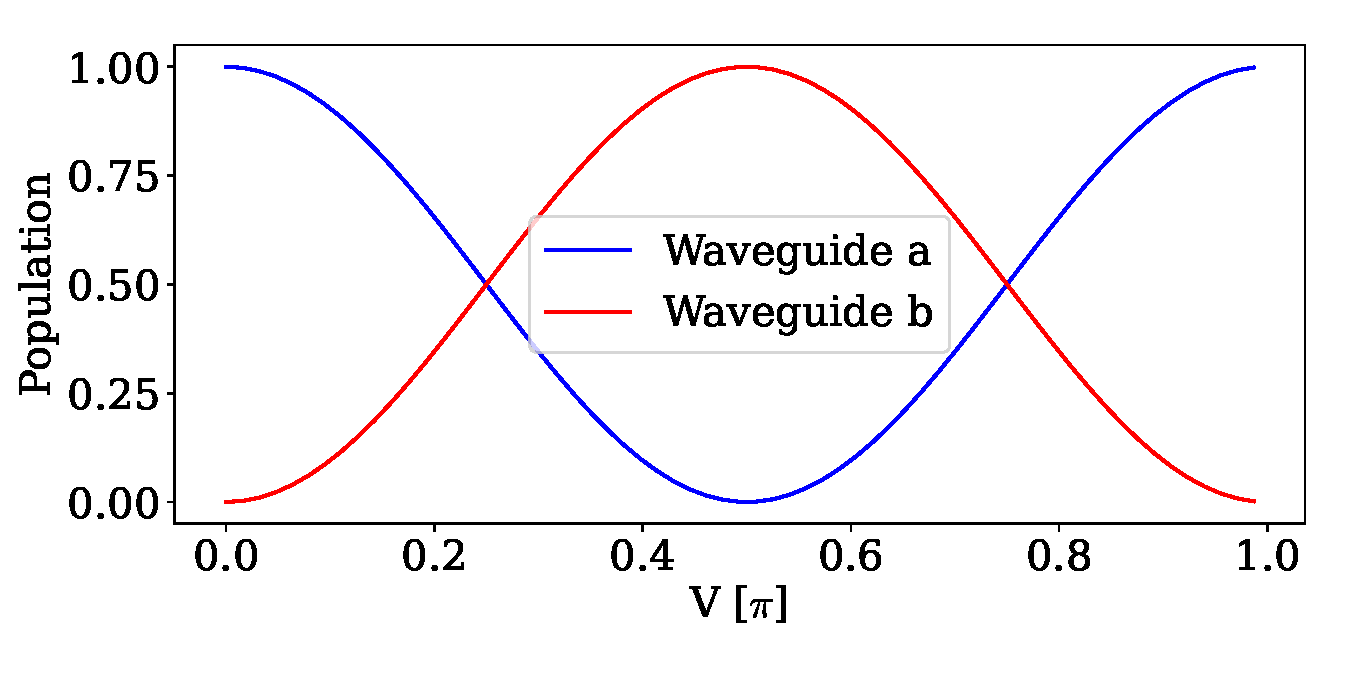
\includegraphics[width=0.6 \linewidth]{figures/beamsplitter_trans.pdf}
    \caption{Population of waveguide $a$ and $b$: $\sum_k \bra{\psi} w_{k,a/b}^\dagger w_{k,a/b} \ket{\psi}$ after interacting for varying coupling strengths $V$. The initial state is a single-photon Gaussian state in waveguide $a$.}
    \label{fig:beamsplitter_trans}
\end{figure}


\begin{figure}[H]
    \centering
    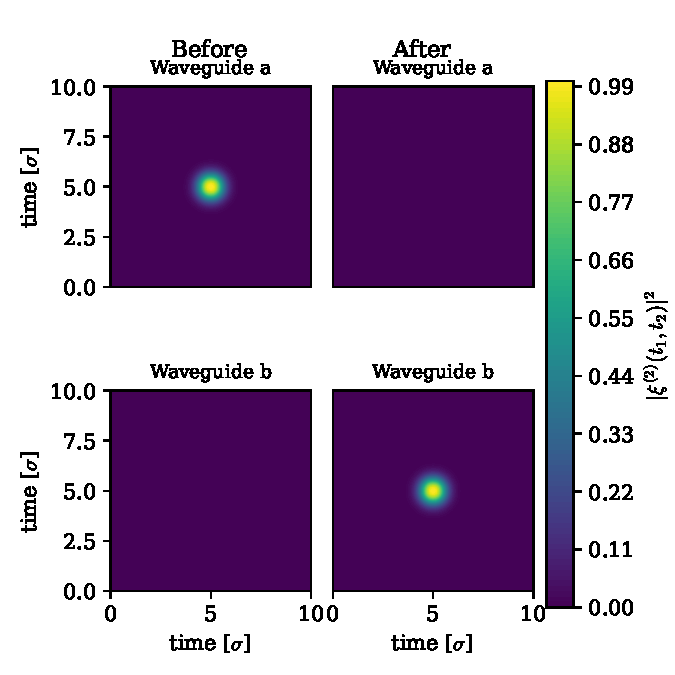
\includegraphics[width=0.6 \linewidth]{figures/swapping_twophoton.pdf}
    \caption{Depiction of two-photon state in waveguide mode $a$ and $b$, before and after interacting respectively. The initial state is a Gaussian two-photon product state in waveguide mode $a$, and the interaction strength is $V=\pi/2$ meaning that we swap the excitation from waveguide mode $a$ to waveguide mode $b$. All plots have been normalized by $\mathrm{max}(\xi^{(2)}(t_1,t_2))$ of the initial state.}
    \label{fig:swapping_twophoton}
\end{figure}

\section{Waveguide Interactions \label{sec:waveguideIO}}
We now revisit the scattering of the emitter considered in Sec.~\eqref{sec:lodahl}, but with $V \neq 0$, meaning that we have a scattering element in the waveguide. Such a scattering element could occur due to a defect in the waveguide but also from a purposefully engineered design (such as two terminating waveguides), see for example photonic crystal fano-lasers \cite{Yu2014FanoSwitching,Yu2017DemonstrationLaser}. Either way, an interesting effect of introducing such a defect is a change in the local density of optical states. This can in turn lead to a change in the emitter lifetime \cite{Joanesarson2020Few-photonGeometries}. This change in the emitter-lifetime can be seen if we consider the self-energy in eq.~\eqref{eq:coupling_definitions}. Immediately, it is clear that the interactions between waveguides change the emitter decay rate as the real part of the self-energy $\Sigma$ describes the decay rate and it depends on the coupling $\mathbf{V}$. If we consider the same configuration as in sec.~\ref{sec:lodahl}, we have $\mathbf{\Gamma} = \begin{pmatrix}
    \sqrt{\gamma_L} \\
    \sqrt{\gamma_R} \\
\end{pmatrix}= \begin{pmatrix}
    \sqrt{\gamma/2} \\
    \sqrt{\gamma/2} \\
\end{pmatrix}$ and $\mathbf{V} =\begin{pmatrix}
    0 & V \\
    V & 0 \\
\end{pmatrix}$. This gives the self-energy:
\begin{equation}
    \Sigma = \gamma/2\left( \frac{1}{1+(V/2)^2} - \frac{i V}{2(1+(V/2)^2)} \right) \label{eq:self}
\end{equation}
We see that in the limit of $V=0$ and thus no interacting waveguides, we recover $\Sigma = \gamma/2$ as expected (the emitter population will decay with $\gamma$). For $V \neq 0$ the self-energy also carries an imaginary factor, corresponding to a frequency shift of emitted photons and the decay rate will also be reduced. We can observe this frequency shift and lifetime increase in the emission spectrum of the emitter.

In standard cavity quantum electrodynamics, the emission spectrum of an emitter can be calculated from the Wiener-Kinchen theory and the correlation function \cite{Steck2007QuantumOptics}:
\begin{equation}
    S(\omega) = \gamma\int \int dt d\tau \expval{a^\dagger(t+\tau) a(t)} \mathrm{e}^{-i\tau \omega} \label{eq:wienerkinchen}
\end{equation}
where $a$ here is the cavity annihilation operator and $\gamma$ the coupling to the environment. If we consider an initially excited emitter $\ket{\psi}(0) = \sigma^\dagger \ket{0}$, we will have equal emission into the two waveguides and only have single-photon states of the form $\ket{\psi}(t \rightarrow \infty) = \frac{1}{\sqrt{2}}\left ( \int \xi(t') w_L^\dagger(t') \ket{\emptyset}+\int \xi(t') w_R^\dagger(t') \ket{\emptyset} \right)$. The emission spectrum in either waveguide is then equivalent $S_L(\omega)=S_R(\omega)=S(\omega)$ and is the Fourier transform of the time wavefunction:
\begin{equation}
    S(\omega) = 2 \pi |\xi(\omega)|^2 = \abs{\int dt \xi(t) \mathrm{e}^{-i\omega t}}^2 \label{eq:spec}
\end{equation}
This is evident if we consider no input field since $w_{out}(t) = \sqrt{\gamma} a(t)$ and thus inserting in \ref{eq:wienerkinchen} we get:
\begin{align}
    S(\omega) &= \int \int dt d\tau \expval{w(t+\tau) w(t)} \mathrm{e}^{-i\tau \omega} = \int \int dt d\tau \xi^*(t+\tau) \xi(t) \mathrm{e}^{-i\tau \omega} = \\
    &\frac{1}{2\pi} \int \int \int \int dt d\tau d\omega^\prime d\omega^{\prime \prime} \xi^*(\omega^{\prime}) \xi(\omega^{\prime \prime}) \mathrm{e}^{-i t (\omega^{\prime\prime }-\omega^{\prime}) t} \mathrm{e}^{-i\tau (\omega - \omega^{\prime})} \\
    & = 2 \pi \int \int d\omega^\prime d\omega^{\prime \prime} \xi^*(\omega^{\prime}) \xi(\omega^{\prime \prime}) \delta(\omega^{\prime \prime}-\omega^{\prime})\delta(\omega-\omega^{\prime}) =  2 \pi |\xi(\omega)|^2
\end{align}
\begin{figure}
    \centering
    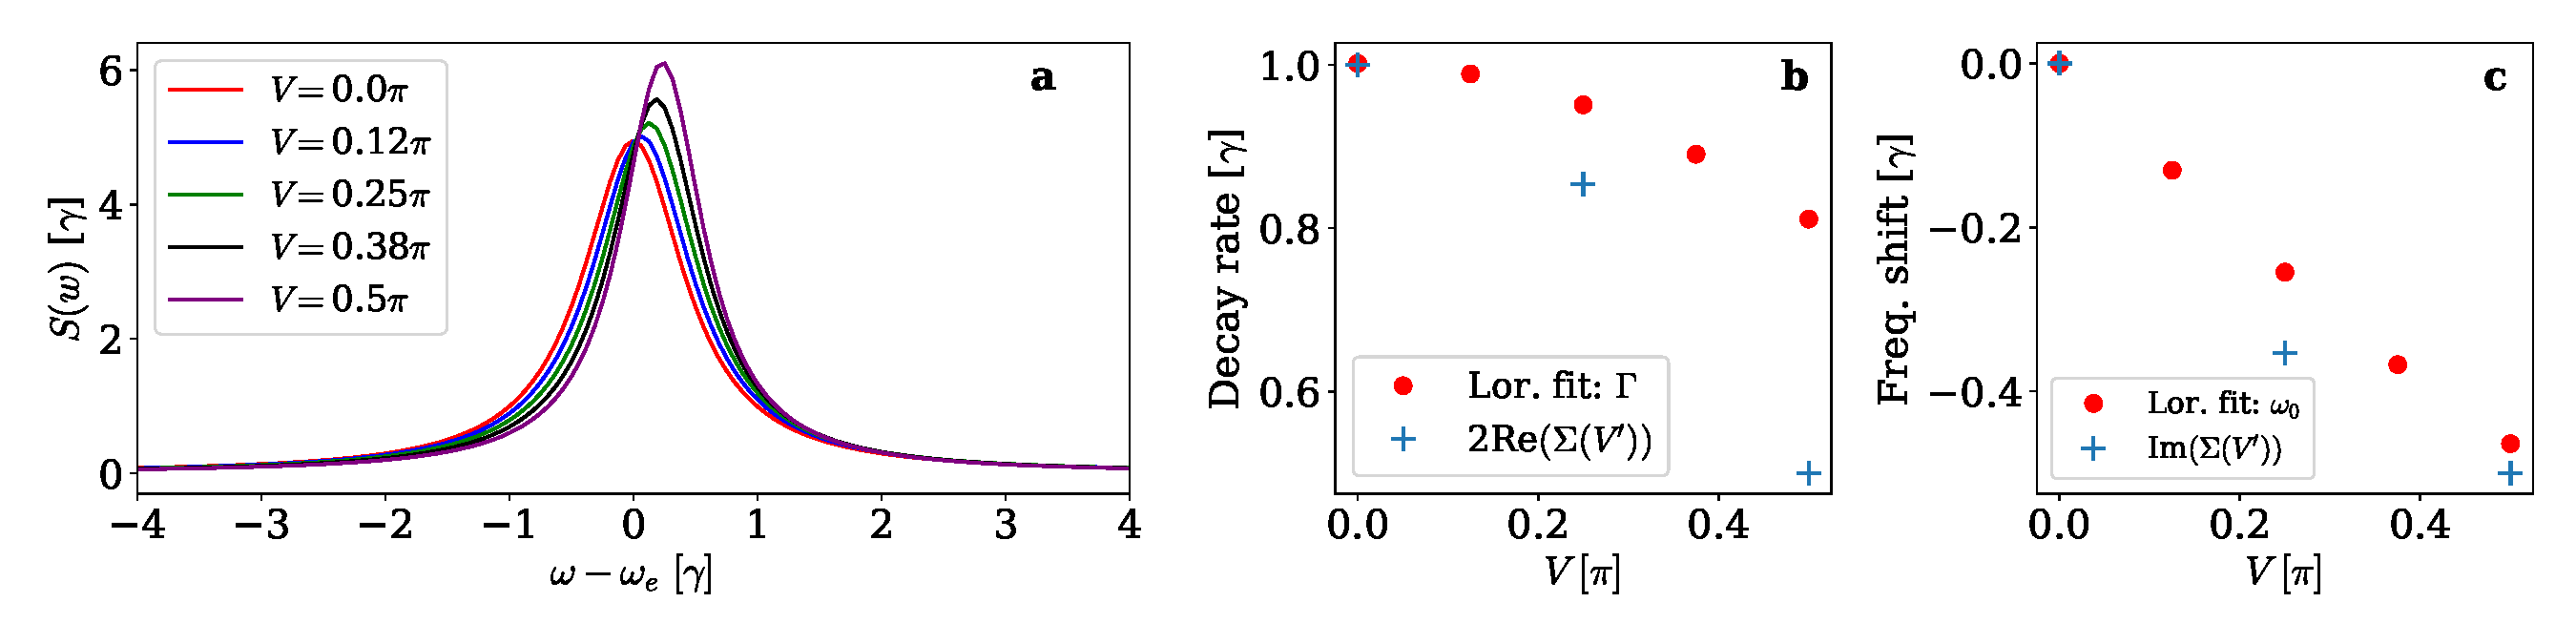
\includegraphics[width=\linewidth]{figures/fanoressonance.pdf}
    \caption{(a) Spectrum as defined in \eqref{eq:spec} for different waveguide couplings $V$. (b) The decay rate (FWHM) of the Lorentzian spectrum in (a) as a function of $V$. The real part of the self-energy $\mathrm{Re}(\Sigma(V'))$ is also plotted for $V'=\{0,2/(1+\sqrt{2}),2\}$ but shown at the points $V =\{0,\pi/4,\pi/2\}$ (for comparison at points with equal input-output relations ). (c) The frequency shift of the Lorentzian in (a) as a function of $V$. $\mathrm{Im}(\Sigma(V'))$ is also shown at the same points as in (b).}
    \label{fig:selfenergy}
\end{figure}


In Fig~\ref{fig:selfenergy}(a), we consider the emission spectrum $S(\omega)$ of an initially excited emitter coupled to two waveguides with the same rate $\gamma/2$ and for varying waveguide interaction strength $V$. As $V$ is increased, we see the effect of the waveguide interaction as a shift in the center frequency. The Full Width Half Max (FWHM) which is related to the emitter emission rate is also seen to decrease for larger $V$ as was expected from the change in the self-energy given by eq.~\eqref{eq:self}. In Fig~\ref{fig:selfenergy} (b)-(c) we plot the FWHM and frequency shift calculated by fitting a Lorentzian on the spectrum in Fig~\ref{fig:selfenergy}(a) as a function of $V$. As we established in sec.~\ref{sec:inputoutput}, there is not a one-to-one correspondence between the $V$ in ref. \cite{Xu2016FanoTransport} and $V$ in our Hamiltonian in eq.~\eqref{eq:lodahl_ham}. Indeed, it was established in sec.~\ref{sec:inputoutput} that we should choose $V = \pi/4$ for an even beamsplitter and $V = \pi/2$ for total reflection whereas in ref. \cite{Xu2016FanoTransport} they find $V=2/(1+\sqrt{2})$ and $V=2$, respectively. This discrepancy would be okay as long as the results for the same physical system are the same. For total reflection $V=2$, the self-energy in eq.~\eqref{eq:self} predicts an emitter emission rate decrease of $2 \mathrm{Re}(\Sigma(2))/(\gamma/2) = 1/2$, however, as is seen in Fig~\ref{fig:selfenergy}, the emission rate is found to decrease by only $\approx 0.8$. A similar, albeit not as large deviation, is also seen in the frequency shift in Fig.~\ref{fig:selfenergy}. This shows a fundamental problem with the time-binned picture. The interaction terms $V/\Delta t w_{k,R}^\dagger w_{k,L}$ and $V/\Delta t w_{k,L}^\dagger w_{k,R}$ which are defined in the time-bin picture does not correspond to the interaction terms in the frequency based Hamiltonian in eq.~\eqref{eq:generalFAN}. In the next section, we propose another method for handling the input-output relations which do not involve the waveguide interaction terms (and thus $V=0$), but instead a rescaling of the waveguide-emitter coupling.

\section{Waveguide Interactions by Rescaling} \label{sec:inferringwaveguide}
Another approach to model the waveguide interactions is to simulate the dynamics without the waveguide interactions and then enforce the input-output relations post-simulation. Indeed, it is argued in ref. \cite{Xu2016FanoTransport} that the system dynamics can be calculated with an effective Hamiltonian $H_{eff} = H_c - i\Sigma a^\dagger a$. In a similar manner, we can omit the waveguide interaction terms if we rescale the waveguide-emitter coupling $\mathbf{\Tilde{\Gamma}} = (\mathbf{I} + \frac{i}{2}\mathbf{V})^{-1} \mathbf{\Gamma}$. Since the emitter-waveguide coupling now can be complex, we have to enforce a Hermitian Hamiltonian by including complex conjugate terms in the coupling:
\begin{equation}
\begin{aligned}
H= H_{\mathrm{s}}+ \sum_{i=1}^N \int d \nu \hbar \nu w_{i}^{\dagger}(\nu) w_{i}(\nu)+\sum_{i=1}^N \hbar \int \frac{d \nu}{\sqrt{2 \pi}}\left(\Tilde{\Gamma}_i^* w_{i}^{\dagger}(\nu) a+ \Tilde{\Gamma}_i a^{\dagger} w_{i}(\nu)\right) \label{eq:modifiedFAN}
\end{aligned}
\end{equation}
where $\Tilde{\Gamma}_i$ is the i'th element of $\Tilde{\mathbf{\Gamma}}$. Notice also that we no longer include waveguide interaction terms in the Hamiltonian. This modification would give a self-energy correction:
\begin{equation}
    \Tilde{\Sigma} = \frac{1}{2} \mathbf{\Tilde{\Gamma}}^\dagger \mathbf{\Tilde{\Gamma}} = \frac{1}{2} \Gamma^T \left ((\mathbf{I} + \frac{i}{2}\mathbf{V})^{-1}\right)^\dagger (\mathbf{I} + \frac{i}{2}\mathbf{V})^{-1} \Gamma = \frac{1}{4}\left (  (\mathbf{I} + \frac{i}{2}\mathbf{V})^{-1} + \left( (\mathbf{I} + \frac{i}{2}\mathbf{V})^{-1}\right)^\dagger \right) = \mathrm{Re}(\Sigma)
\end{equation}
where we used that $\mathbf{C}^\dagger = \mathbf{C}^*$ and that $(\mathbf{I} + i/2 \mathbf{V})^{-1} = 1/2(\mathbf{I}+\mathbf{C})$. With the normalized coupling, we thus recover the real part of the self-energy correction. We can then explicitly include the imaginary part by adding a detuning term to our system Hamiltonian: $\Tilde{H_{\mathrm{c}}} = H_{\mathrm{c}} + a^\dagger a \mathrm{Im}(\Sigma)$. With this, the modified input-output relations become:
\begin{align}
& \frac{d}{d t} a= -i\left[a, \Tilde{H_{\mathrm{c}}} \right] -\mathrm{Re}(\Sigma) a + \Tilde{\mathbf{k}}^T \mathbf{W}_{\mathrm{in}} \label{eq:scaledIO1} \\
& \widetilde{\mathbf{W}}_{\text {out }}(t)= \mathbf{\Tilde{C}} \mathbf{W}_{\mathrm{in}}(t)+a(t)\Tilde{\mathbf{d}} \label{eq:scaledIO2}
\end{align}
where $\Tilde{\mathbf{d}} = -i \left(\left(\mathbf{I}+\frac{i}{2} \mathbf{V}\right)^{-1} \right)^* \mathbf{\Gamma}$, $\Tilde{\mathbf{k}} = -i \left(\left(\mathbf{I}+\frac{i}{2} \mathbf{V}\right)^{-1} \right) \mathbf{\Gamma}$, and $\Tilde{\mathbf{C}} = \mathbf{I}$. Eqs.~\eqref{eq:scaledIO1} and \eqref{eq:scaledIO2} do, however, not fulfill the constraints that ensure flux conservation and time reversal symmetry. Specifically, $\Tilde{\mathbf{k}} = \Tilde{\mathbf{d}}$ is not satisfied. This can, however, be restored if we multiply eq.~\eqref{eq:scaledIO2} with $\mathbf{C}$ and we thus arrive at:
\begin{align}
\mathbf{C} \widetilde{\mathbf{W}}_{\text {out }}(t)= \mathbf{C} \mathbf{W}_{\mathrm{in}}(t)+a(t)\Tilde{\mathbf{k}}
\end{align}
where we used that $\mathbf{C} \Tilde{\mathbf{d}} = - i/2 \mathbf{C} (\mathbf{I}+\mathbf{C}^*) = \Tilde{\mathbf{k}}$. If we thus define $\mathbf{C} \widetilde{\mathbf{W}}_{\text {out }} \equiv \mathbf{W}_{out}$, we can simulate the dynamics of the system with the rescaled couplings and system Hamiltonian $\Tilde{H}$ but with no waveguide coupling $V=0$, to obtain $\widetilde{\mathbf{W}}_{\text {out }}$. After the simulation, we then apply $\mathbf{C}$ to get $\mathbf{W}_{out}$. Since we are working in the Schrodinger picture, our output state will be $\ket{\psi}_{\mathrm{out}} = \sum_i \int \widetilde{W}_{out,i}^\dagger \ket{\emptyset}$ and we thus apply $C^\dagger$ to the output state such that: $C^\dagger \ket{\psi}_{\mathrm{out}} = \sum_{i,j} \int C_{i,j}^\dagger \widetilde{W}_{out,i}^\dagger \ket{\emptyset} = \sum_i \int W_{out,i}^\dagger \ket{\emptyset}$. This is shown for a single-photon state but can also be generalized to two-photon states.

\

\begin{figure}
    \centering
    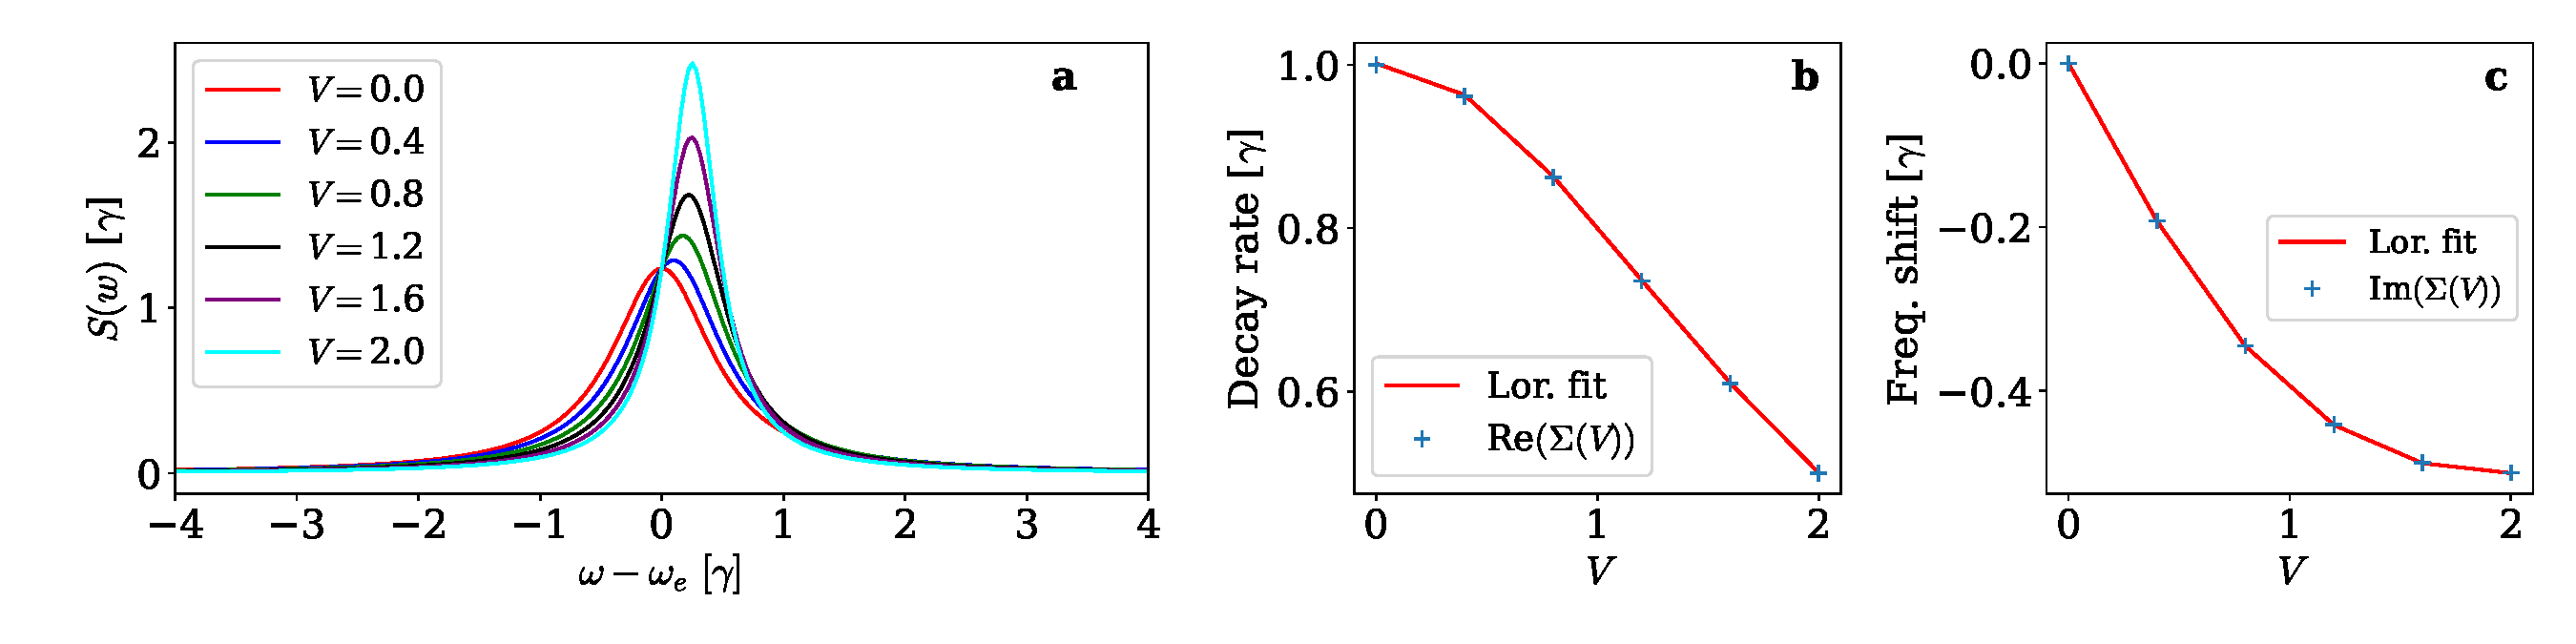
\includegraphics[width = \linewidth]{figures/fanoressonanceIO.pdf}
    \caption{Same as Fig~\ref{fig:selfenergy}, but calculated using the rescaling method explained in sec.~\ref{sec:inferringwaveguide}}
    \label{fig:DecayIO}
\end{figure}

Using this approach, we are able to predict the correct increase in emitter lifetime and shift, as is shown in Fig.~\ref{fig:DecayIO}. However, this does not prove that we are able to correctly capture the scattering of an incoming wavepacket. To prove this, we consider how a Gaussian pulse scatters off the emitter for $V=\{0,2/(\sqrt{2}+1),2\}$ corresponding to the case considered in sec.~\ref{sec:lodahl}, a 50:50 beamsplitter, and a fully reflecting scattering element. This configuration is also studied in detail in Ref. \cite{Joanesarson2020Few-photonGeometries}. In Fig~\ref{fig:fanoIO}, we consider a pulse with a width of $\Tilde{\sigma} = 1.14 (1+(V/2)^2)^{-1}$ corresponding roughly to the pulse width that excites the emitter to the maximum possible probability of 0.4 \cite{Joanesarson2020Few-photonGeometries}. The pulse is also detuned with a frequency of $\Tilde{\omega} = \mathrm{Im}(\Sigma)$ corresponding to the shift in the emitter emission due to the scattering element V. We show the time wavefunction $\xi(t)$, frequency wavefunction $\xi(\omega)$, and the excitation probability as a function of time. We see that except for different widths of the emitted field, the wavefunctions are equivalent for $V=0$ and $V=2$, except that the transmitted and reflected fields are swapped. In the case of a beamsplitter $V=2/(1+\sqrt{2})$, the output fields are asymmetric in frequency space but with the same excitation probability of exactly 0.5. This asymmetry is particularly interesting as it leads to a Fano resonance where there is a sharp drop in the transmission of different frequencies. We show this in Fig.~\ref{fig:fano_transmission}, where we plot the ratio between the amplitude of the input state $\xi(\omega)$ and the scattered state in the reflected and transmitted mode, respectively. We see that for frequencies around $\omega \approx -1/2 \gamma$, we have total reflection, and for frequencies $\omega \approx 1/2 \gamma$, we have total transmission. These results agree with the results obtained from analytically derived scattering matrices in ref. \cite{Joanesarson2020Few-photonGeometries}.       

\begin{figure}[H]
    \centering
    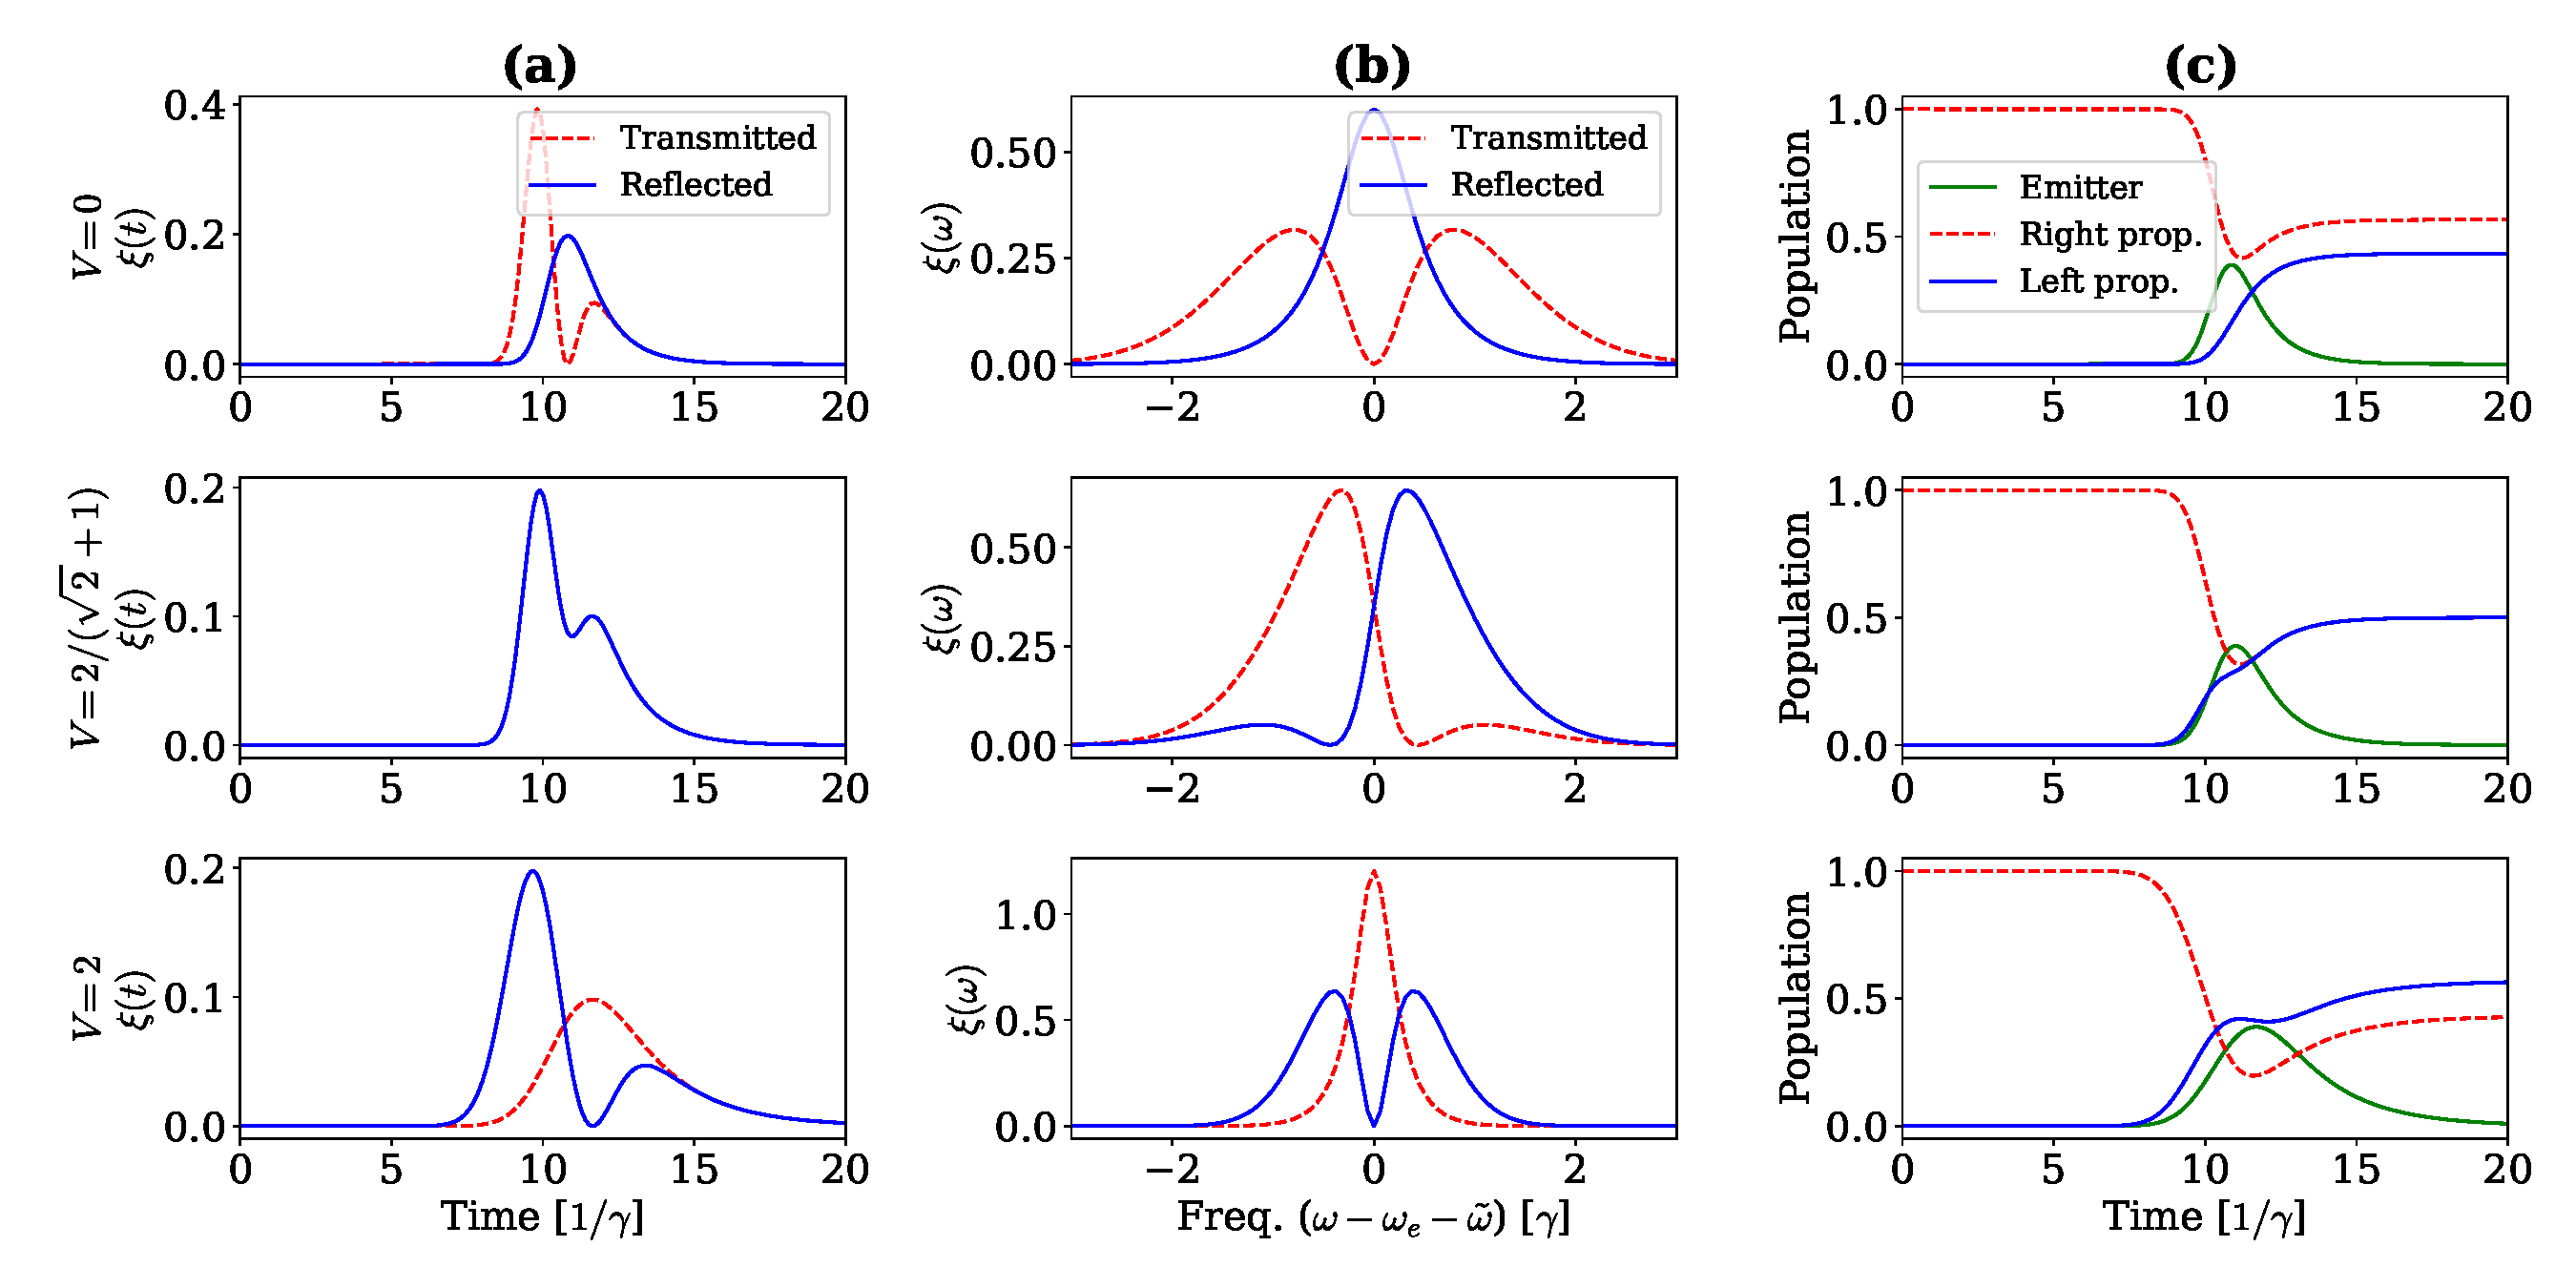
\includegraphics[width=\linewidth]{figures/Fanoscattering.pdf}
    \caption{Column (a): The time-wavefunction $\xi(t)$ as a function of time. Column (b) The frequency wavefunction $\xi(\omega)$, notice that the frequency axis is shifted with the frequency $\Tilde{\omega} = \mathrm{Im}(\Sigma)$ arising from the waveguide interactions. Column (c) the population of the emitter, left, and right propagating fields. The first row shows the case of $V=0$ corresponding to no scattering element, the second row shows $V=2/(1+\sqrt{2})$ corresponding to a beamsplitter, and the third row $V=2$ corresponding to a fully reflecting element.  }
    \label{fig:fanoIO}
\end{figure}


We have thus shown that we can model few-photon transport in waveguides with internal coupling. This is a valuable extension of the collision optics picture as it can allow a fundamental study of the transport properties of different waveguide geometries. We showed that allowing for direct interactions between the waveguide modes in the Hamiltonians leads to errors in self-energy changes of the local emitter system. Rather we found that we can stay within the limitations of collision optics by renormalizing the coupling and then ensure the correct waveguide coupling post-simulation. With the numerical approach implemented here, it is simple to consider more complex systems. From here, a natural extension of the study would, therefore, be to consider how a two-photon pulse scatters on a waveguide with internal coupling and analyzing systems where the complexity has previously prevented analytical derivations.

\begin{figure}
    \centering
    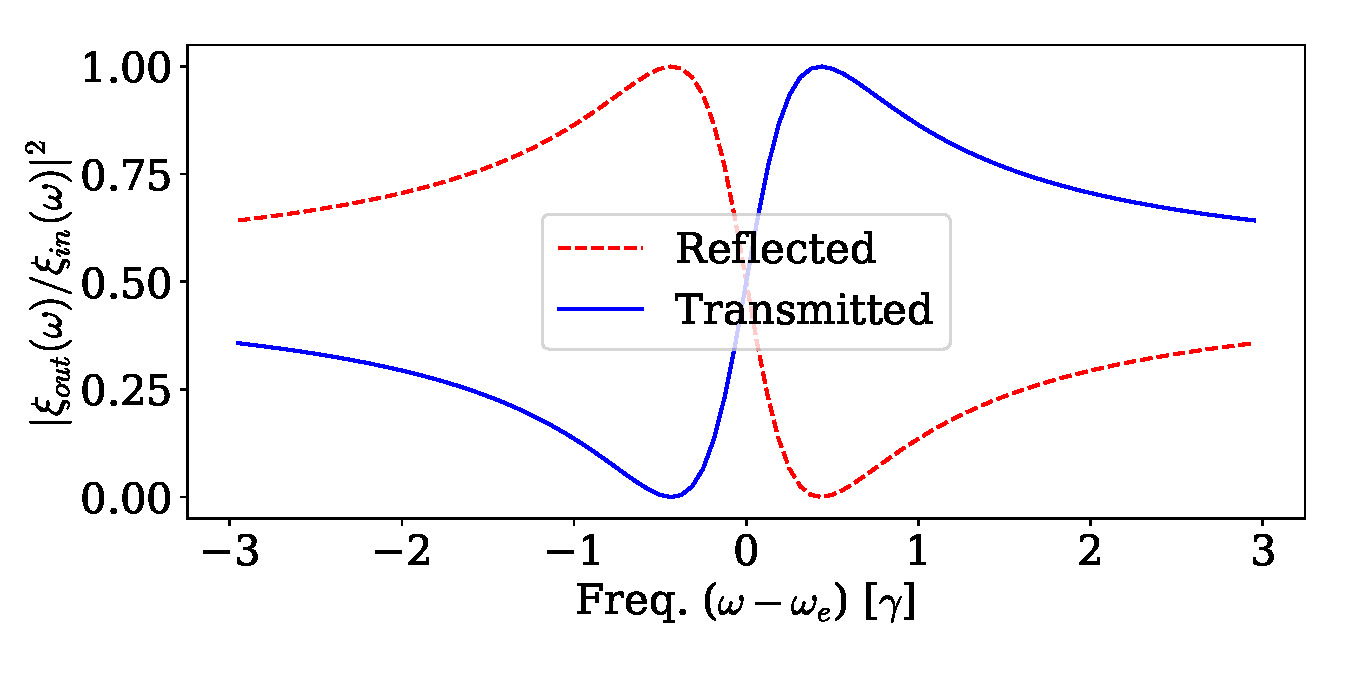
\includegraphics[width=0.5 \linewidth]{figures/fano_transmission.pdf}
    \caption{The transmission/reflection rate for the beamsplitter $V=2/(\sqrt{2}+1)$ as a function of frequency $\omega$. }
    \label{fig:fano_transmission}
\end{figure}
%Introduce multiple waveguides mathematically

%Beamsplitter example

%Lodahl scattering example

%Barrett and Kok introduction. 

%Simulate using waveguideQED full method.

%Simulate using detectors instead and confirm same results.

%Understand fidelity. 

%\chapter{Entanglement of qubits}
%In the previous chapters, we considered how propagating quanta of radiation scatter on different quantum systems. In this chapter, we are instead going to consider how we can mediate entanglement between two 
spatially separated matter qubits. This is an interesting topic as it plays a vital role in numerous quantum technology applications, such as quantum repeaters (and ultimately quantum networks) \cite{}. Photons can here mediate interaction between qubits, and entanglement can be achieved through bell state measurements on beamsplitters.

When the two emitters are identical and operate without dephasing noise, the emitted photons are indistinguishable, and their wavefunctions exhibit a complete overlap. Due to the Hong Ou Mandel effect\cite{MANDEL}, the "which path information" is thus erased when combined on a beamsplitter, and consequently, entanglement can be achieved. However, in realistic scenarios, differences between the emitters introduce variations in the respective wavefunctions of the emitted photons, leading to imperfect overlaps. The photons become distinguishable, and the fidelity of the entanglement is reduced. 

To address this challenge, various protocols have been proposed that try to maximize the fidelity of the entanglement while still keeping a high success probability. There are numerous ways to simulate these protocols, and typically a master equation approach can be applied \cite{Barrett2004EfficientOptics}.

In this chapter, we will show how we can simulate such protocols using the time-binned photon formalism. The approach enables straightforward calculation of the success probabilities, the photon indistinguishability, and the protocol fidelity since we have access to the complete wavefunction of the emitted photons. 

\section{Entanglement of two emitters}

In ref. \cite{Barrett2004EfficientOptics} they propose a scheme to entangle two distant matter qubits. The qubits consist of three states: Two longlived lover excited states $\ket{\uparrow}$ and $\ket{\downarrow}$ and one excited state $\ket{e}$ that can undergo the transition $\ket{e} \rightarrow \ket{\downarrow}$ by emitting a photon. The transition $\ket{e} \rightarrow \ket{\uparrow}$ is not permitted due to selection rules. Each qubit is placed inside a cavity where the cavity mode matches the frequency of the transition $\ket{e} \rightarrow \ket{\downarrow}$.

Before we go over the scheme proposed in ref. \cite{Barrett2004EfficientOptics}, we consider the evolution of an excited state in both qubits. We thus have the initial state $\ket{\psi(t=0)} = \ket{e,0,\emptyset}_a \ket{e,0,\emptyset}_b$, where $\ket{e,0,\emptyset}_{a/b}$ denotes an excited qubit $\ket{e}$, an empty cavity $\ket{0}$, and an empty waveguide $\ket{\emptyset}$ at site a/b . Assuming sufficient time $t_{wait}$ has passed, all excitations will have leaked out of the emitter/cavity system and into the waveguide. We can thus describe the system at this point as:
\begin{equation}
     \ket{\psi(t_{wait})} = \sum_k \sum_j \xi_a(t_k)\xi_b(t_j) 
 w_{k,a}^\dagger w_{j,b}^\dagger \ket{\downarrow,0,\emptyset}_a \ket{\downarrow,0,\emptyset}_b
\end{equation}
where $\xi_a(t_k)$ and $\xi_b(t_j)$ are the amplitudes of the emission from site $a$ and $b$ at time $t_k$ and $t_j$, respectively and $w_{k,a/b}^\dagger$ the creation operator of a photon in waveguide $a/b$ in time-bin $k$.  

If the emitted photons subsequently interfere on a beamsplitter, the waveguide operators transform as $w_{k,a}^\dagger \rightarrow \frac{1}{\sqrt{2}} \left [ w_{k,a}^\dagger + w_{k,b}^\dagger \right ]$ and $w_{k,b}^\dagger \rightarrow \frac{1}{\sqrt{2}} \left [ w_{k,a}^\dagger - w_{k,b}^\dagger \right ]$. The state after the interaction is then: 
\begin{align}
    \ket{\psi(t_{wait})}  &\xrightarrow{BS} \frac{1}{2} \sum_k \sum_j \xi_a(t_k)\xi_b(t_j) \left [w_{k,a}^\dagger+w_{k,b}^\dagger \right ] \left [w_{j,a}^\dagger-w_{j,b}^\dagger \right ]  \ket{\downarrow,0,\emptyset}_a \ket{\downarrow,0,\emptyset}_b \\
    &=  \frac{1}{2} \sum_k \sum_j \xi_a(t_k)\xi_b(t_j) \left [w_{k,a}^\dagger w_{j,a}^\dagger - w_{k,a}^\dagger w_{j,b}^\dagger + w_{k,b}^\dagger w_{j,a}^\dagger - w_{k,b}^\dagger w_{j,b}^\dagger \right ] \ket{\downarrow,0,\emptyset}_a \ket{\downarrow,0,\emptyset}_b
\end{align}

The probability of detecting two photons in waveguide $a$ at time $t_i$ and $t_j$ after the beamsplitter interaction can then be calculated by using the projector:
\begin{equation}
P_{aa}(t_i,t_j) = w_{i,a}^\dagger w_{j,a}^\dagger \ket{\downarrow,0,\emptyset}_a \ket{\downarrow,0,\emptyset}_b \bra{\downarrow,0,\emptyset}_a \bra{\downarrow,0,\emptyset}_b w_{i,a} w_{j,a}    
\end{equation}
where the probability is then given as (we here leave out $\ket{\downarrow,0}$ since they just fall out and immediately notice that all terms are zero except the one containing $w_{k,a}^\dagger w_{j,a}^\dagger$):
\begin{align}
    &\bra{\psi(t_{wait})} P_{aa}(t_i,t_j) \ket{\psi(t_{wait})} = \\
    &\frac{1}{4} \sum_{k,l,m,n} \xi_a^*(t_k)\xi_b^*(t_l) \xi_a(t_m)\xi_b(t_n) \bra{\emptyset}_a \bra{\emptyset}_b w_{j,a} w_{k,a} w_{i,a}^\dagger w_{j,a}^\dagger  \ket{\emptyset}_a \ket{\emptyset}_b \bra{\emptyset}_a \bra{\emptyset}_b w_{i,a} w_{j,a} w_{l,a}^\dagger w_{m,a}^\dagger  \ket{\emptyset}_a \ket{\emptyset}_b \\
    & = \frac{1}{4} \sum_{k,l,m,n}  \xi_a^*(t_k)\xi_b^*(t_l) \xi_a(t_m)\xi_b(t_n) (\delta_{il}\delta_{jk}+\delta_{ik}\delta_{jl})(\delta_{im}\delta_{in}+\delta_{in}\delta_{im}) \\
    &= \frac{1}{4} (\xi_a^*(t_i)\xi_b^*(t_j) + \xi_a^*(t_j)\xi_b^*(t_i))(\xi_a(t_i)\xi_b(t_j) +\xi_a(t_j)\xi_b(t_i)) = \abs{\xi_a(t_i)\xi_b(t_j) +\xi_a(t_j)\xi_b(t_i)}^2
\end{align}
The total probability of observing two photons in waveguide $a$ $P_aa$ is then the sum of all the above projections two-time projections:
\begin{equation}
   P_{aa} = \frac{1}{4} \sum_i \sum_j \abs{( \xi_a(t_i)\xi_b(t_j) + \xi_a(t_j)\xi_b(t_i))}^2
\end{equation}

Similarly, we would have the probability of observing one photon in waveguide $a$ and one photon in waveguide $b$ $P_{ab}$:
\begin{equation}
   P_{ab} = \frac{1}{4} \sum_i \sum_j \abs{( \xi_a(t_i)\xi_b(t_j) - \xi_a(t_j)\xi_b(t_i))}^2
\end{equation}
If the two emitted photons are identical, $\xi_a(t_i)\xi_b(t_j) =  \xi_a(t_j)\xi_b(t_i)$ and we would thus never observe two photons in different waveguides after the beamsplitter. This is the Hong-Ou-Mandel effect. 

The total probability of having detector + clicking thus is:

\begin{equation}
    P(D_+) =  \sum_j \sum_m \frac{1}{2} \abs{\frac{1}{2} ( \xi_a(t_j)\xi_b(t_m) + \xi_a(t_m)\xi_b(t_j))}^2 + \abs{ \frac{1}{2} ( -\xi_a(t_m) \xi_b(t_j) +\xi_a(t_j) \xi_b(t_m))}^2
\end{equation}


Detecting a second photon again leads to:

\begin{align}
    D_\pm \ket{\psi(t_{wait})} &\rightarrow D_\pm D_\pm \ket{\psi(t_{wait})} \\
    & = \frac{1}{2} \sum_k \sum_j \left( \pm \xi_a(t_k)\xi_b(t_j)  \ket{\downarrow, 0, \emptyset}_a \ket{\downarrow,0,\emptyset}_b \pm \xi_a(t_j)\xi_b(t_k) \ket{\downarrow,0,\emptyset}_a \ket{\downarrow,0,\emptyset}_b \right )   
\end{align}

From this it is evident that if $\xi_a(t)=\xi_b(t)$ for all times then observing a click in two different detectors is not possible (as expected). 

The intital state is, however, slithgly more complicated since the initial state is the following entangled state:

\begin{equation}
    \ket{\psi} = \frac{1}{2}(\ket{e}_a+\ket{\uparrow}_a)\ket{0,\emptyset}_a(\ket{e}_b+\ket{\uparrow}_b)\ket{0,\emptyset}_b
\end{equation}

After sufficient time, the excited states $\ket{e}_{a/b}$ has decayed and emitted a photon into the waveguide. We here have the (un-normalized) state:

\begin{align}
    \ket{\psi} &= \sum_k  \xi_b(t_k) \ket{\uparrow,0,\emptyset}_a \ket{\downarrow,0,1_k}_b + \sum_k \xi_a(t_k) \ket{\downarrow,0,1_k}_a \ket{\uparrow,0,\emptyset}_b \\
    & + \sum_k \sum_j \xi_a(t_k)\xi_b(t_j) \ket{\downarrow,0,1_k}_a\ket{\downarrow,0,1_j}_b + \ket{\uparrow,0,\emptyset}_a\ket{\uparrow,0,\emptyset}_b
\end{align}

After the first detection, we thus have:

\begin{align}
    \ket{\psi} \rightarrow D_\pm \ket{\psi} &=  \sum_k \xi_a(t_k) \ket{\downarrow,0,\emptyset}_a \ket{\uparrow,0,\emptyset}_b \pm \xi_b(t_k) \ket{\uparrow,0,\emptyset}_a \ket{\downarrow,0,\emptyset}_b \\
    &+ \sum_k \sum_j \xi_a(t_k)\xi_b(t_j) \ket{\uparrow,0,\emptyset}_a\ket{\uparrow,0,1_j}_b \pm \ket{\uparrow,0,1_k}_a\ket{\uparrow,0,\emptyset}_b 
\end{align}

In the paper, they then take into account the fact that realistic photo detectors cannot capture two photons arriving in a quick succession. They simulate this by allowing no more information to be gained, claiming that the resulting state would be:

\begin{equation}
    \rho \propto \ket{\psi_\pm} \bra{\psi_\pm} + \ket{\uparrow,0,\emptyset}_a\ket{\uparrow,0,\emptyset}_b \bra{\uparrow,0,\emptyset}_a\bra{\uparrow,0,\emptyset}_b
\end{equation}

where $\ket{\psi_\pm} = \ket{\downarrow,0,\emptyset}_a \ket{\uparrow,0,\emptyset}_b \pm \ket{\uparrow,0,\emptyset}_a \ket{\downarrow,0,\emptyset}_b$. Ideally, we would like not to simulate density matrices, and perhaps this is where the montecarlo trajectory comes into the picture. Do we split up in two paths from here. One where we have projected onto the entangled state and one where we project onto everything else?



\section{Entanglement heralding}
\begin{figure}[H]
    \centering
    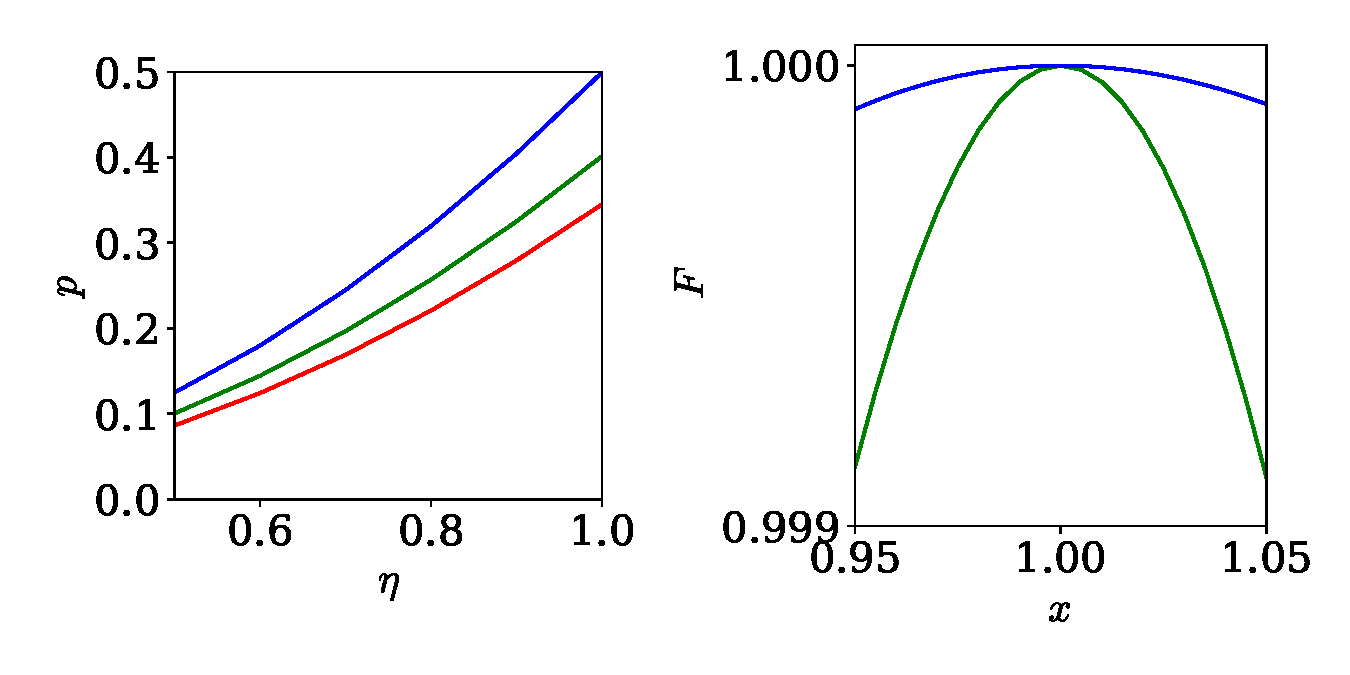
\includegraphics[width = 0.5 \linewidth]{figures/barett_fig2.pdf}
    \caption{Caption}
    \label{fig:my_label}
\end{figure}

\begin{figure}[H]
    \centering
    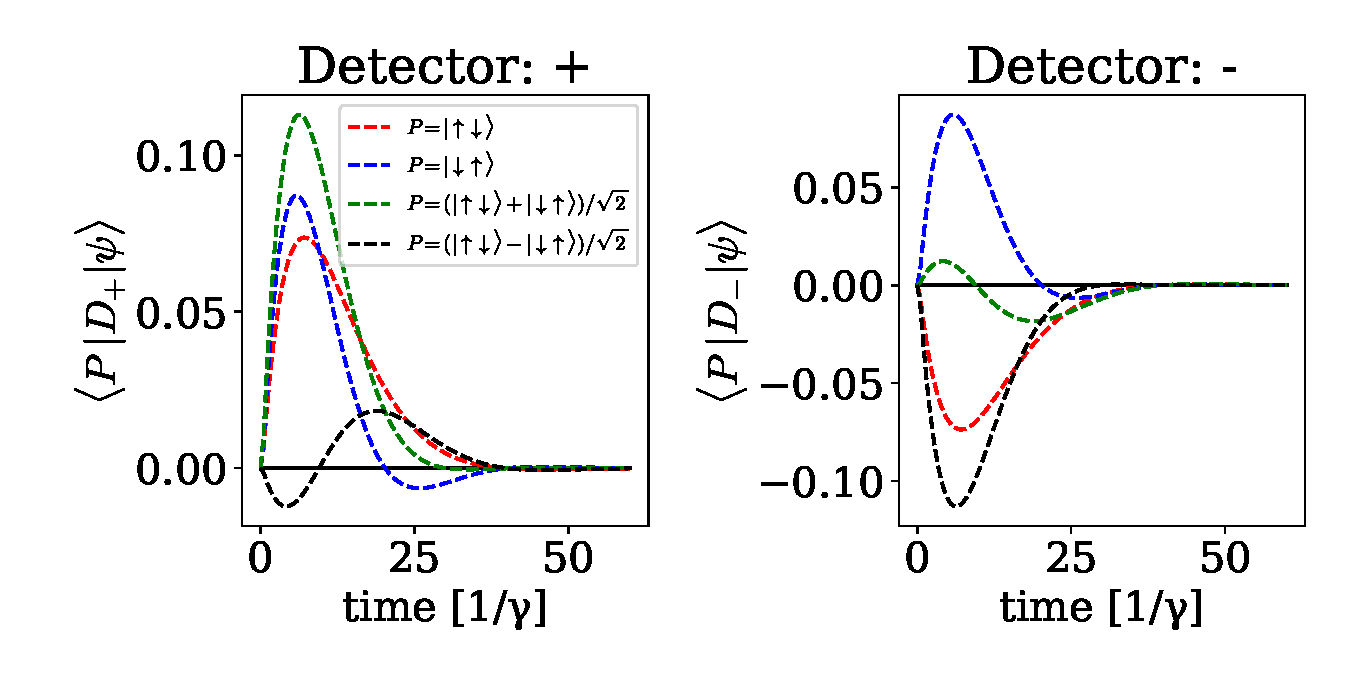
\includegraphics[width = 0.5 \linewidth]{figures/barett_uneven_g_first_detection.pdf}
    \caption{Uneven g, first round of detection.}
    \label{fig:my_label}
\end{figure}

\begin{figure}[H]
    \centering
    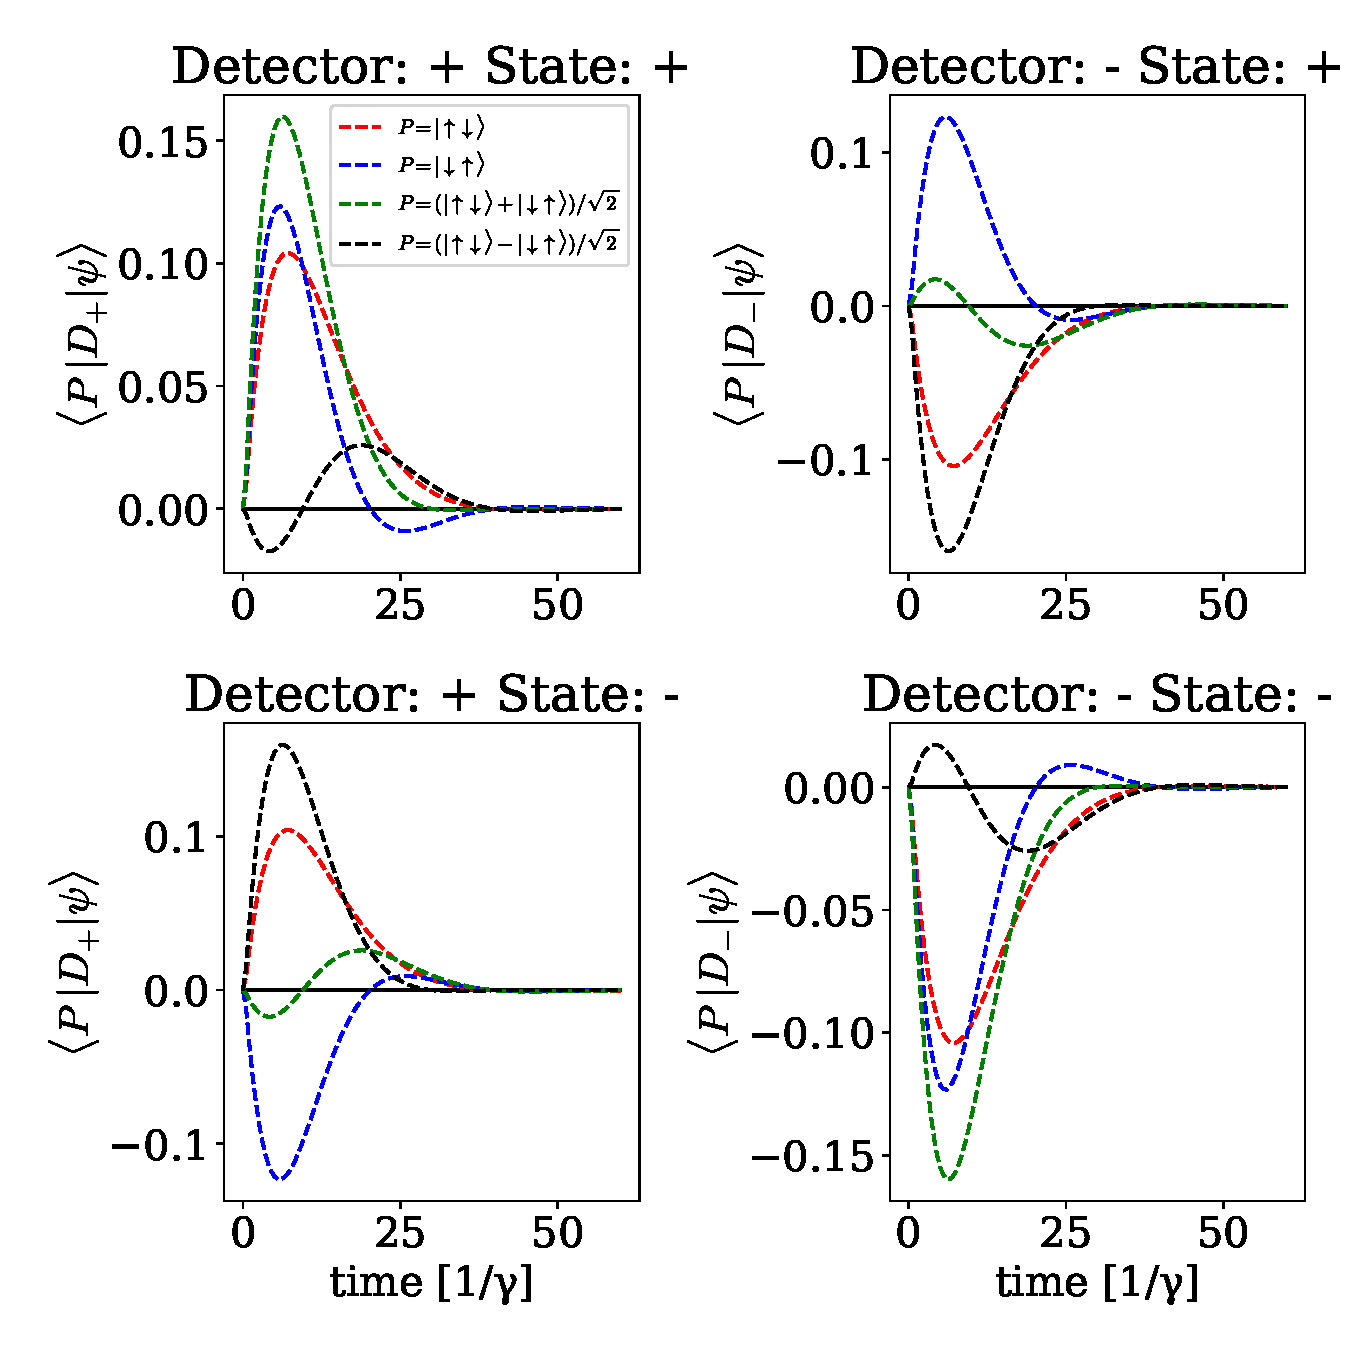
\includegraphics[width = 0.5 \linewidth]{figures/barett_uneven_g_second_detection.pdf}
    \caption{Uneven g, second round}
    \label{fig:my_label}
\end{figure}

\begin{figure}[H]
    \centering
    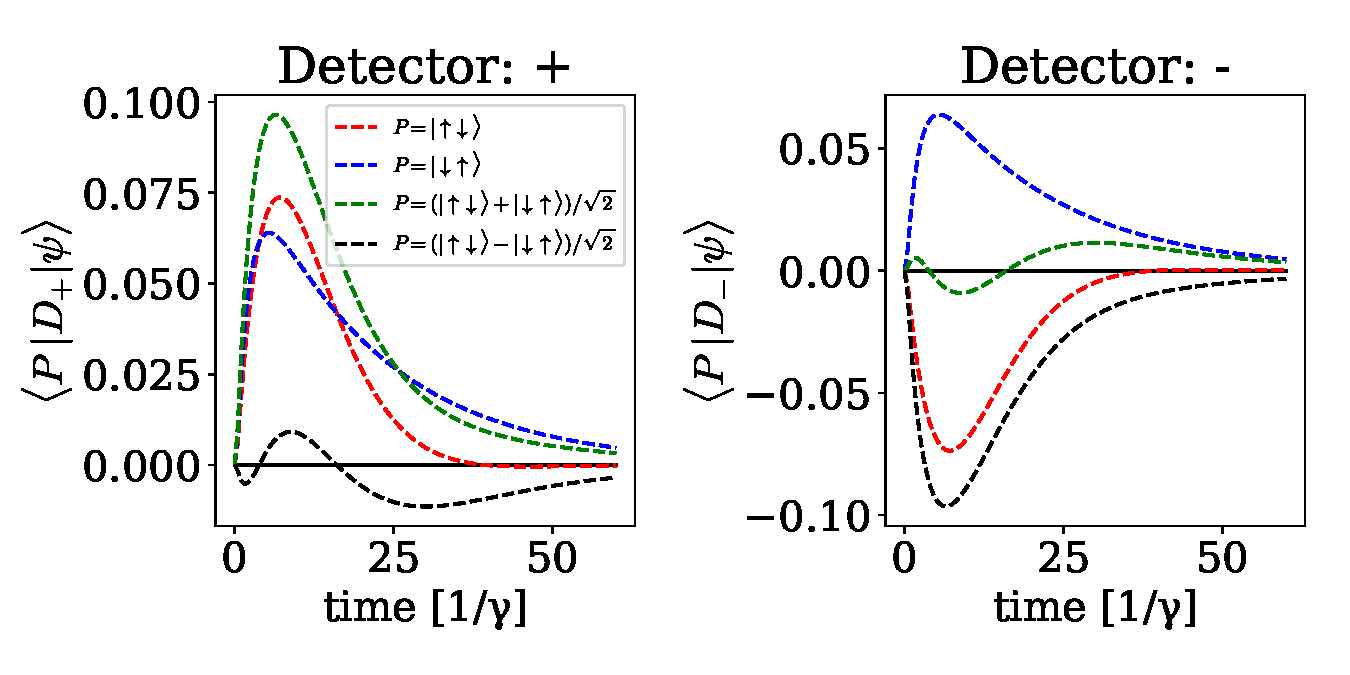
\includegraphics[width = 0.5 \linewidth]{figures/barett_uneven_kappa_first_detection.pdf}
    \caption{Uneven $\kappa$ first round}
    \label{fig:my_label}
\end{figure}

\begin{figure}[H]
    \centering
    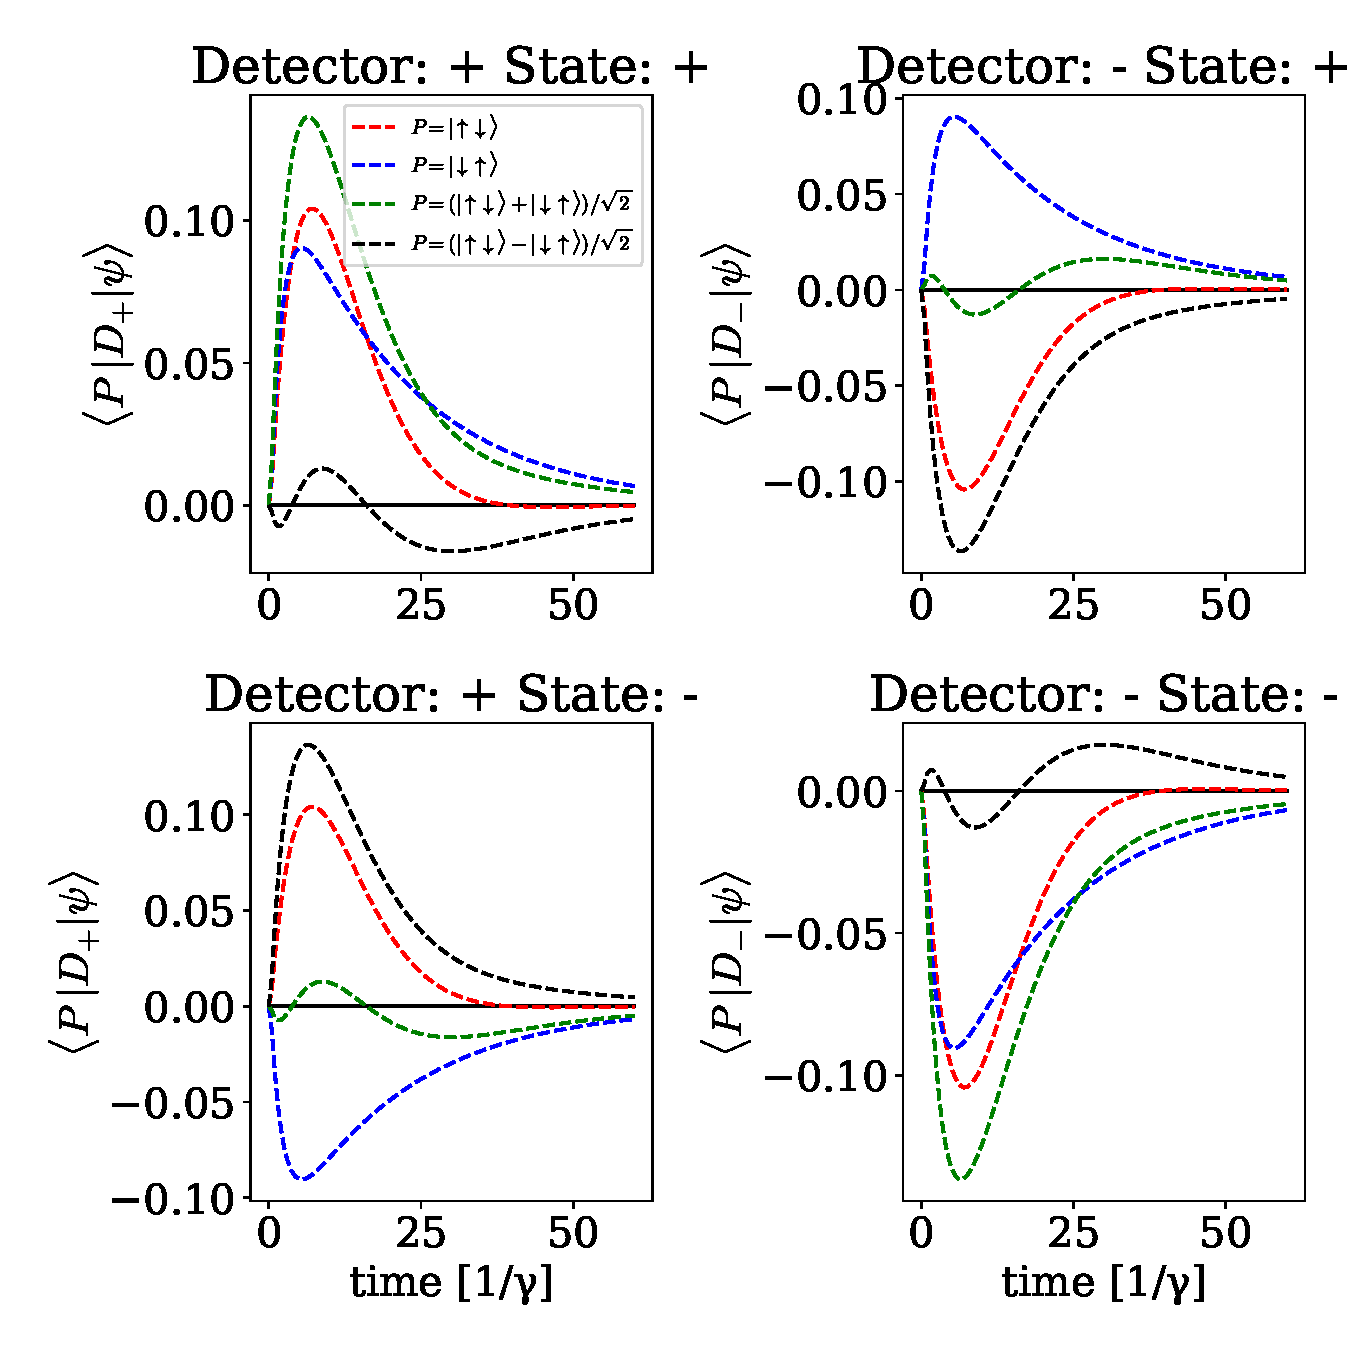
\includegraphics[width = 0.5 \linewidth]{figures/barett_uneven_k_second_detection.pdf}
    \caption{Uneven $\kappa$ second round}
    \label{fig:my_label}
\end{figure}


\section{Detection in waveguide using Monte-Carlo trajectories}

At each timeindex $t_k$ the interaction between the cavity and the waveguide is given by $i \sqrt{\gamma/dt} ( a w_k^\dagger - a^\dagger w_k)$ where $w_k$ is the annihilation operator for a photon in the waveguide in the timebin $t_k$. If we assume that the photon is detected in the waveguide the timebin after it was emitted (this seems reasonable?), the jump operator for the detection event is $w_{k-1}$. The jump operator would thus be changing at each timestep to be the annihilation operator for the previous step. Question is, what should the associated rate with this jump be? In this case we are not describing the leakage of a cavity but a photon hitting a detector. The intuitive answer to the rate would be the probablility of having a photon in that timebin times the timestep: $\abs{\xi_{k-1}}^2 \mathrm{dt}$ (with our state being $\ket{\psi}=\sum_k \sqrt{\mathrm{dt}}\ \xi_k w_k^\dagger \ket{\emptyset}$. But this is exactly just the overlap $\abs{\xi_{k-1}}^2=\expval{w_{k-1}^\dagger w_{k-1} }{\psi}/\mathrm{dt}$ which I guess is already included in the monte-carlo trajectory formalism? So maybe the rate is just unity (one). However, when I run simulations I notice that there is a high chance of no detection event happening at all! This should never be the case. We know that we will have a jump/detection, just not when the jump happens. This leads me to think that the above reasoning is wrong and that I'm missing something. Should the jump operator or rate somehow be cumulative so that we ensure that a jump happens or should the jump operator itself be different?

\section{Waveguide interactions}
If we consider two waveguides interacting we then have:
\begin{equation}
    H_{int} = V \left ( \int \frac{dk}{\sqrt{2 \pi}} \int \frac{dk'}{\sqrt{2 \pi}} w_{1}(k)^\dagger w_{2}(k') + \int \frac{dk}{\sqrt{2 \pi}} \int \frac{dk'}{\sqrt{2 \pi}} w_{2}(k')^\dagger w_{1}(k)\right )
\end{equation}
In the interaction picture with
\begin{equation}
    H_0 = \sum_\mu \int_{-\infty}^\infty d k k w^\dagger_\mu(k)w_\mu(k)
\end{equation}
we have the transformation: 
\begin{equation}
    \mathrm{e}^{i t H_0} w_\mu(k) \mathrm{e}^{-i t H_0} = \mathrm{e}^{-ikt} w_\mu(k)
\end{equation}
and thus:
\begin{equation}
    \mathrm{e}^{i H_0 t } H_{int} \mathrm{e}^{-i H_0 t } = V \left ( \int \frac{dk}{\sqrt{2 \pi}} \int \frac{dk'}{\sqrt{2 \pi}} \mathrm{e}^{ikt} w^\dagger_{1}(k) \mathrm{e}^{-ik't} w_{2}(k') + \int \frac{dk}{\sqrt{2 \pi}} \int \frac{dk'}{\sqrt{2 \pi}} \mathrm{e}^{ik't} w^\dagger_{2}(k') \mathrm{e}^{-ikt} w_{1}(k)\right )
\end{equation}
Introducing the fourier transformed operators $w_\mu(t) = \frac{1}{\sqrt{2 \pi}} \int_{-\infty}^\infty d k \mathrm{e}^{-ikt} w_{\mu}(k)$ we have: 
\begin{equation}
    H_{int}(t)  = \mathrm{e}^{i H_0 t } H_{int} \mathrm{e}^{-i H_0 t } = V \left ( w_1^\dagger(t) w_2(t) + w_2^\dagger(t) w_1(t)\right )
\end{equation}
Similarly, the unitary evolution operator becomes (for now let's exclude $H_s$ and $V(t)$):
\begin{equation}
    U_n = \mathrm{e}^{- i \int_{t_{n-1}}^{t_n} dt' H_{int}(t)} = \mathrm{e}^{- i \int_{t_{n-1}}^{t_n} dt' V \left ( w_1^\dagger(t') w_2(t') + w_2^\dagger(t') w_1(t')\right )}
\end{equation}
In previous examples we make the discretization:
\begin{equation}
    w_{\mu,n} = \frac{1}{\sqrt{\Delta t}} \int_{t_{n-1}}^{t_n} d t' w_{\mu}(t')
\end{equation}
And thus the natural extension would be:
\begin{equation}
    U_n = \mathrm{e}^{- i \Delta t V \left ( w^\dagger_{1,n} w_{2,n} + w_{2,n}^\dagger w_{1,n}\right )}
\end{equation}
But this is not equivalent since:
\begin{equation}
   \int_{t_{n-1}}^{t_n} dt' w_1^\dagger(t') w_2(t') \neq  w^\dagger_{1,n} w_{2,n} = \frac{1}{\sqrt{\Delta t}} \int_{t_{n-1}}^{t_n} d t' w^\dagger_{1}(t') \frac{1}{\sqrt{\Delta t}} \int_{t_{n-1}}^{t_n} d t' w_{2}(t')
\end{equation}





Defining then: 

\begin{align}
c_{\mathrm{in}}(t) & =\int \frac{d k}{\sqrt{2 \pi}} c_{\mathrm{in}, k}\left(t_0\right) e^{-i k\left(t-t_0\right)}, \\
c_{\mathrm{out}}(t) & =\int \frac{d k}{\sqrt{2 \pi}} c_{\mathrm{out}, k}\left(t_1\right) e^{-i k\left(t-t_1\right)},
\end{align}

with $t_0 \rightarrow - \infty$ and $t_1 \rightarrow \infty$

and thus equivalently:

\begin{align}
c_{\mathrm{in,k}}\left(t_0\right) & =\int \frac{d k}{\sqrt{2 \pi}} c_{\mathrm{in}}(t) e^{-i k\left(t-t_0\right)}, \\
c_{\mathrm{out,k}}\left(t_1\right) & =\int \frac{d k}{\sqrt{2 \pi}} c_{\mathrm{out}}(t) e^{-i k\left(t-t_1\right)},
\end{align}

$\int_{-1}^{1} e^{-(x-x_0)^2} dx = \frac{\sqrt{\pi}}{2} \left[ \mathrm{erf}\left(\frac{1-x_0}{\sqrt{2}}\right) - \mathrm{erf}\left(\frac{-1-x_0}{\sqrt{2}}\right) \right]
$


We get:

\begin{equation}
    H =  V \left ( \int \frac{dk}{\sqrt{2 \pi}} \int \frac{dk'}{\sqrt{2 \pi}} c_{in,k}^\dagger c_{out,k'} + \int \frac{dk}{\sqrt{2 \pi}} \int \frac{dk'}{\sqrt{2 \pi}} c_{out,k}^\dagger c_{in,k'} \right )
\end{equation}


\section{Waveguide Interaction}

Assume we have two waveguides with corresponding creation and annihilation operators $\omega_1$ and $\omega_2$. They interact via:
$$
\begin{aligned}
& H_I(t)=\sum_k f_k(t) V\left(w_1^{+}\left(t_k\right) w_2\left(t_k\right)+w_2^{+}\left(t_k\right) w_1\left(t_k\right)\right) \\
& \text { Where } f_k(t)= \begin{cases}1 \text { if } t=t_k \\
0 \text { else }\end{cases}
\end{aligned}
$$
We note that $\left[H_I(t), H_I\left(t^{\prime}\right)\right]=0$
That can probably be exploited in some way to show that we can do something like:
$$
\begin{aligned}
\quad \partial_t w_1\left(t_k\right) & = [ w_1,H_I ] = -\frac{i}{\hbar}\left[w_1\left(t_k\right), V\left(w_1^{\dagger}\left(t_k\right) w_2(t_k)+w_2^{\dagger}\left(t_k\right) w_1\left(t_k\right)\right)\right] \\
& =-\frac{i}{\hbar} V w_2\left(t_k\right)
\end{aligned}
$$
and $\quad \partial_t w_2\left(t_k\right)=-\frac{i}{\hbar} V w_1\left(t_k\right)$
Thus: $W=\left[\begin{array}{l}w_1\left(t_k\right) \\ w_2\left(t_k\right)\end{array}\right] \quad \partial_t W=\left(\begin{array}{cc}0 & -\frac{i}{\hbar} V \\ -\frac{i}{\hbar} V & 0\end{array}\right) W$

Furthermore we have:

$$
\begin{aligned}
&m:=\left[\begin{array}{cc}
0 & -\mathrm{I} V \\
-\mathrm{I} V & 0
\end{array}\right]\\
&\exp( M)=\left[\begin{array}{cc}
\cos (V) & -\mathrm{I} \sin (V) \\
-I \sin (V) & \cos (V)
\end{array}\right]
\end{aligned}
$$


\begin{equation}
    \ket{\psi} = \int_{t_0}^{t_{end}} \mathrm{d}t \ \xi_1(t) w_1^\dagger(t) \ket{\emptyset}_1\ket{\emptyset}_2 + \int_{t_0}^{t_{end}} \mathrm{d}t \ \xi_2(t) w_2^\dagger(t) \ket{\emptyset}_1\ket{\emptyset}_2
\end{equation}

\begin{equation}
    H = i \sqrt{\kappa_1/dt}(\sigma^\dagger w_1 - \sigma w_1^\dagger)+i \sqrt{\kappa_2/dt}(\sigma^\dagger w_2 - \sigma w_2^\dagger) + i V(w_1 ^\dagger w_2 - w_2^\dagger w_1) 
\end{equation}

\begin{equation}
    C_{lm}^{(2)}(t_1,t_2) = \abs{\psi_l(t_1)}^2 \abs{\psi_m(t_2)}^2
\end{equation}


\begin{align}
    & a \ket{n} = \sqrt{n} \ket{n-1} \\
    & a^\dagger \ket{n} = \sqrt{n+1} \ket{n+1}
\end{align}

\begin{align}
    \ket{n} = \begin{pmatrix} 0 \\ \vdots \\ 1  \\ \vdots \\ 0  \end{pmatrix}
\end{align}

\begin{align}
a = \begin{pmatrix}
0 & 0 & 0 & \cdots \\
1 & 0 & 0 & \cdots \\
0 & \sqrt{2} & 0 & \cdots \\
0 & 0 & \sqrt{3} & \cdots \\
\vdots & \vdots & \vdots & \ddots
\end{pmatrix}
\end{align}


$w_k^\dagger \ket{\emptyset} = \ket{1_k} \ \ \\ \ \\ $ 

$\frac{d}{dt} \mathbf{\Bar{x}} = \bar{\bar{a}} \mathbf{\Bar{x}}$ \ \ \\ \ \ \\ \ \

${H}\ket{\psi} = i\hbar\frac{\partial }{\partial t} \ket{\psi}$


\chapter{Waveguides with feedback}
In this chapter, we consider waveguide systems with non-Markovian dynamics. Such memory effects can arise when the emitted light is reflected back into the system or when considering two spatially separated emitters. Waveguide systems with memory effects constitute a challenging class of problems because knowledge of the emitted field is inherently required to capture the correct feedback. As alluded to in the introduction, many numerical Waveguide QED approaches such as the SLH \cite{Kiilerich2019Input-OutputPulses,Kiilerich2020QuantumRadiation} or master equation approaches \cite{Baragiola2012N-PhotonSystem} do not describe the emitted field in its entirety. Treating feedback mechanisms in these frameworks is therefore challenging. As also mentioned in the ch.~\ref{ch1}, matrix-product states can therefore be used to represent the entire state of the waveguide efficiently and allow for non-markovian effects to be introduced \cite{ArranzRegidor2021ModelingModel}. However, the complexity involved with matrix-product states is substantial and it can be hard to understand the underlying machinery. The time-binned waveguide picture employed in our framework is, on the other hand, a simpler and more intuitive approach, where the calculations are less of a "black box". This comes with the price of restricting the total number of excitations to two (for the moment). In the future, the total number of photons could be extended to allow for more photons, but the numerical costs will grow quickly, and at some point, the more efficient matrix product states will be a better solution. 

In the following, we discuss how to implement these effects in the WaveguideQED.jl framework. We consider a semi-infinite waveguide where one side has a mirror and feeds back emitted light to the system. We show that we correctly predict known effects such as excitation trapping and also consider how single-photon and two-photon pulses scatter.  



\begin{figure}[H]
    \centering
    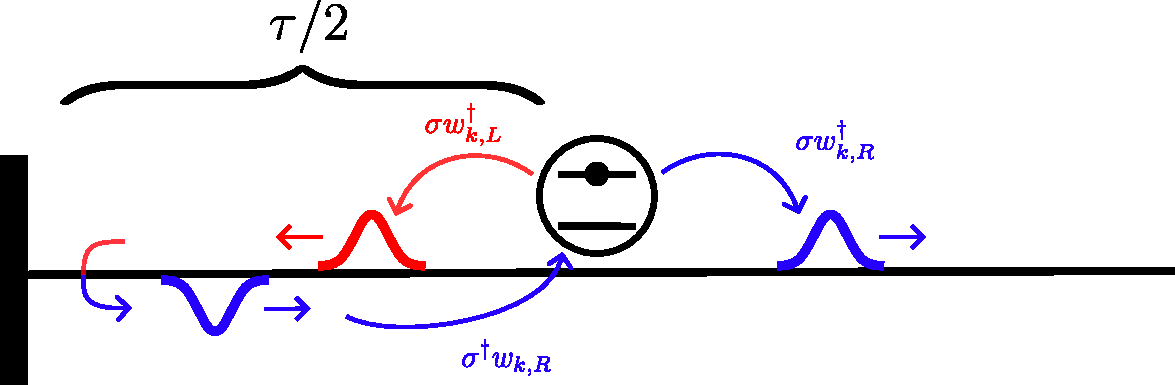
\includegraphics[width = 1 \linewidth]{figures/mirror_feedback.pdf}
    \caption{Illustration of a two-level system coupled to a semi-infinite waveguide, where one end of the waveguide terminates at a mirror reflecting incoming photons. The left propagating mode (red) propagates for a time $\tau/2$ until it gets reflected into the right propagating mode (blue) that returns to the emitter after a total time of $\tau$.}
    \label{fig:feedback_sketch}
\end{figure}

\section{Semi-Infinite Waveguide}
We consider a Semi-Infinite Waveguide terminating with a mirror in one end, as also depicted in Fig.~\ref{fig:feedback_sketch}. The mirror will here introduce a face shift $\phi$, but also an excitation emitted in the left mode will, after a delay time of $\tau/2$, be reflected into the right mode and thus, after a total delay time of $\tau$ hit the emitter again. The left and right propagating modes are, however, symmetrical \cite{ArranzRegidor2021ModelingModel}, and one can instead think of a single mode wrapping around the emitter. The waveguide is thus a "horseshoe", and the emitter couples to two points of the horseshoe. This is also illustrated in Fig.~\ref{fig:horseshoe}. With this mental picture, there is only one propagating mode, and we describe the interaction through the Hamiltonian \cite{Whalen2019CollisionTrajectories}:
\begin{equation}
    H_k = \mathrm{e}^{i \phi} \sqrt{\gamma/2\Delta t} \left( \sigma^\dagger w_{k} + \sigma w_{k}^\dagger \right) + \sqrt{\gamma/2\Delta t} \left( \sigma^\dagger w_{k+\Tilde{\tau}} + \sigma w_{k+\Tilde{\tau}}^\dagger \right) \label{eq:tls_feedback}
\end{equation}
where $\Tilde{\tau} = \tau/\Delta t$ is the index necessary to introduce a time-delay of $\tau$. Note that it is the operator $w_{k+\Tilde{\tau}}$ that never "sees" the emitted photon again (thus corresponding to the left propagating mode in Fig~\ref{fig:feedback_sketch}), whereas the operator $w_{k}$ experiences the emitted photon from $\Tilde{\tau}$ time steps ago (and thus corresponds to the right propagating mode in Fig.~\ref{fig:feedback_sketch}).  $w_{k}^\dagger$ and $w_{k}$ thus carry the phase factor $\mathrm{e}^{i \phi}$ from the mirror. 

\begin{figure}[H]
    \centering
    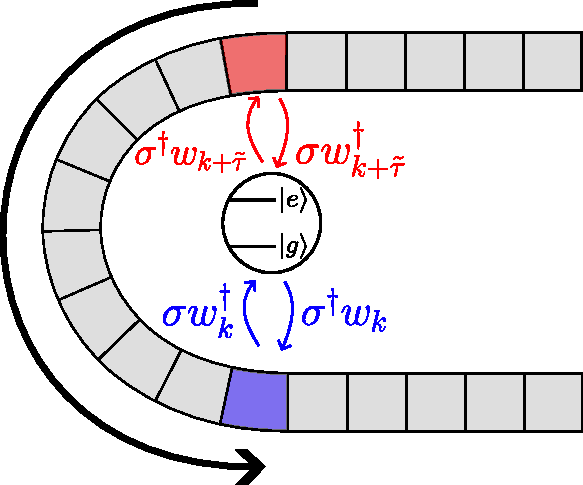
\includegraphics[width=0.5\linewidth]{figures/horseshoe.pdf}
    \caption{Numerical illustration of the semi-infinite waveguide, where the emitter couples to two points of the waveguide such that previous emission re-interacts with the emitter. $\Tilde{\tau} = \tau/\Delta t$ is here the index that induces the time delay $\tau$ between the emission and reabsorption of the emitted pulse. The blue and red interaction carries a phase difference of $\phi$.}
    \label{fig:horseshoe}
\end{figure}

With the Hamiltonian in eq.~\eqref{eq:tls_feedback}, we can simulate how an initially excited emitter decays. In Code Sample \ref{ls:time_delay_code}, we show how to construct the time delayed operator $w_{k+\Tilde{\tau}}$. Notice the simplicity in setting up the simulation. We define two time-delayed operators in the Hamiltonian, and suddenly we can simulate non-Markovian effects. The rest of the code and functions used are the same as previously, allowing for a painless user experience. This modality or separation of features also allows for great customization in the systems that can be studied. The software is thus truly versatile and not just well-defined to solve a restricted set of pre-defined problems.

In Fig.~\ref{fig:tls_feedback}, we plot the population of the emitter as a function of time. We consider two mirror phases $\phi = \pi$ and $\phi = 0$ both $\tau = 1/\gamma$. For reference, we also plot the case of $\tau = \infty$, meaning no memory effects. We see two very distinct population evolutions depending on the phase of the mirror. For $\phi = 0$, the reflected photon interferes constructively with the emission of a photon in the right propagating mode from the emitter.  This leads to a faster decay of the emitter, which is evident by comparing with the case of $\tau=\infty$. Thus, The emitter emits a photon that leads to stimulated emission with itself! With $\phi = \pi$, we instead have destructive interference, and the excitation can never escape to the right. This leads to excitation being trapped, and the system goes to a steady state where the emitter has a constant population of $\approx 0.5$. 




\begin{listing}[H]
\begin{minted}[
frame=lines,
framesep=2mm,
baselinestretch=1.2,
bgcolor=LightGray,
fontsize=\small,
linenos,
escapeinside=||,
mathescape=true
]{julia}
times = 0:0.1:12 #Times for setting up waveguide basis
dt = times[2]-times[1]
be = FockBasis(1)
bw = WaveguideBasis(1,1,times)
sdw = create(be) |$\otimes$| destroy(bw)
wds = destroy(be) |$\otimes$| create(bw)

gamma = 1 #Decay rate of emitter
delay_time = 1 #In units of gamma
phi = pi #Mirror phase

#Creat delayed waveguide operator with delay keyword
sdw_delay = create(be) |$\otimes$| destroy(bw;delay=delay_time/dt)
wds_delay = destroy(be) |$\otimes$| create(bw;delay=delay_time/dt)

H = exp(i*phi)*sqrt(gamma/2/dt)*(sdw+wds)+sqrt(gamma/2/dt)*(sdw_delay+wds_delay)

#Operator for emitter population
sd = create(be) |$\otimes$| identityoperator(bw)
s = destroy(be) |$\otimes$| identityoperator(bw)
n = ad*a
function ne_exp(time,psi)
    expect(n,psi)
end

psi_initial = fockstate(be,1) |$\otimes$| zerophoton(bw) #Initial state
times_sim = 0:0.1:10 #Simulation time has to be smaller than times due to delay. 
tout, ne_pi = waveguide_evolution(times_sim, psi_initial, H,fout=ne_exp)
\end{minted}
\caption{Code for simulating delayed feedback in the waveguide illustrated in Fig.~\ref{fig:horseshoe}. Lines 1-6 set up the standard waveguide basis, emitter basis, and waveguide operators. Lines 8-10 set up the parameters for the simulation. Lines 13-14 set up the delayed waveguide operators $\sigma^\dagger w_{k+\Tilde{\tau}}$ and $\sigma w^\dagger_{k+\Tilde{\tau}}$ by using the keyword \code{delay}. The rest simulates the population of the emitter.}
\label{ls:time_delay_code}
\end{listing}


\begin{figure}[H]
    \centering
    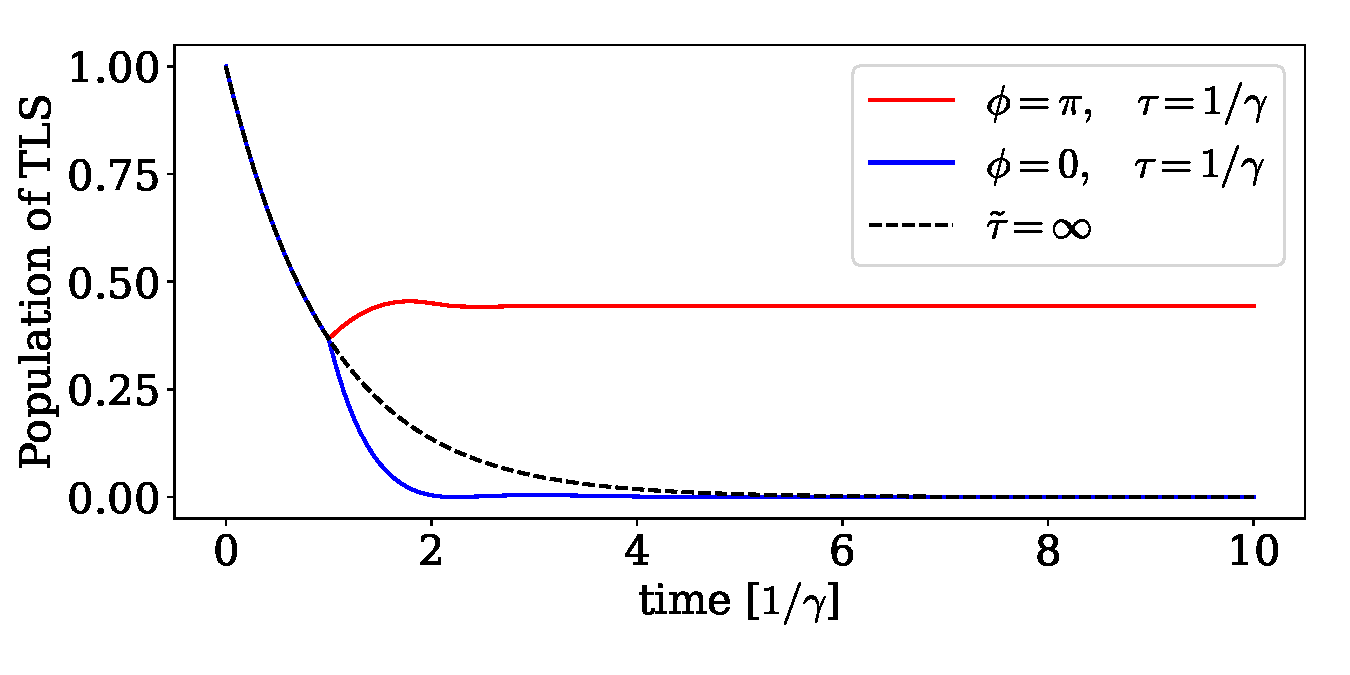
\includegraphics[width = 0.5\linewidth]{figures/tls_mirror_pop.pdf}
    \caption{The population of a two-level system coupled to a semi-infinite waveguide with a mirror in one end. The mirror is located such that a round trip from the emitter to the mirror takes $\tau$ time, and the mirror induces a phase change of $\phi = 0$ and $\phi = \pi$, respectively. This leads to either a faster decay of the emitter or excitation trapping, where the emitter does not decay further. The case where the mirror is placed infinitely far away $\tau = \infty$ is also shown for reference.}
    \label{fig:tls_feedback}
\end{figure}

We can also simulate how an incoming single-photon Gaussian state scatters off on this system. In Fig.~\ref{fig:onephoton_pulse}, we consider an initial Gaussian single photon state: $\ket{\psi}_{in} = \sum_k \xi^{(1)}(t_k) \sqrt{\Delta t} \ket{1_k}$ with $\xi^{(1)}$ defined in eq.~\eqref{eq:gaussian}. The pulse has a width of $\sigma = 0.5 / \gamma$, and the delay from the mirror is still $\tau = 1/\gamma$. For reference, we also show the case of a single-sided cavity ($\tau = 0$) as studied in ch.~\ref{ch2} and \ref{ch3}. In Fig.~\ref{fig:onephoton_pulse}(a), we show the two-level-system population as a function of time. Most noticeably, we do not see an excitation trapping, no matter the phase change of the mirror. A stronger reflection of the pulse when the mirror phase change is $\phi = \pi$ (red) is seen as a much lower excitation probability of the emitter. The first part of the pulse here reflects off the mirror and interferes with the later part of the pulse leading to a strong reflection. This is evident in Fig.~\ref{fig:onephoton_pulse}(b), where we consider the scattered wavefunctions. For $\phi = \pi$, the reflected wavefunction has a Gaussian output shape with a strongly suppressed "tail." For reference, the single-sided scattered wavefunction (black $\tau=0$) shows a distorted shape with two peaks. For $\phi = 0$, the single-photon output state is even more distorted, with an extra peak arising, most likely due to multiple interactions with the emitter.  


\begin{figure}[H]
    \centering
    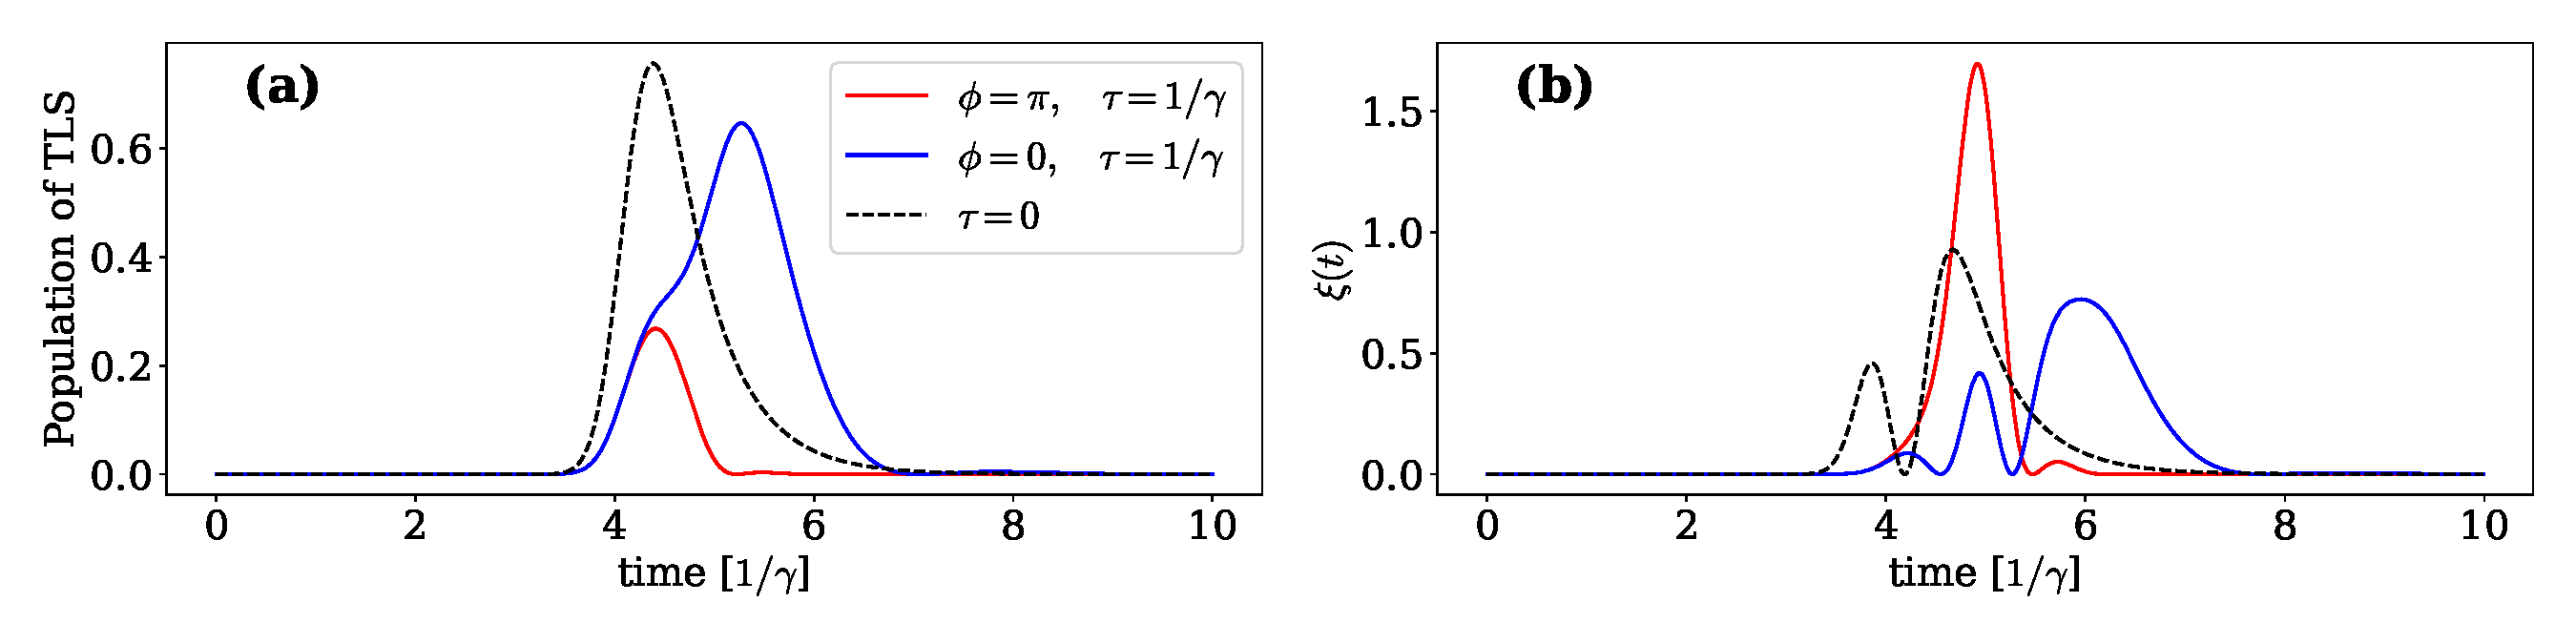
\includegraphics[width=\linewidth]{figures/pulse_wf.pdf}
    \caption{(a) Same as Fig~\ref{fig:tls_feedback}, but with an incoming Gaussian single-photon state with width $\sigma = 0.5 /\gamma$. (b) The scattered wavefunction after the incoming Gaussian pulse has interacted with the emitter and mirror. }
    \label{fig:onephoton_pulse}
\end{figure}

Finally, we can instead consider a two-photon Gaussian pulse on the semi-infinite waveguide with a mirror. In Fig~\ref{fig:twophoton_mirror}(a), we show the two-photon scattered wavefunction for a two-photon Gaussian product state $\ket{\psi}_{in} = \sum_k \sum_j \xi^{(1)}(t_k)\xi^{(1)}(t_j) \Delta t w_k^\dagger w_j^\dagger \ket{\emptyset}$ with the same parameters as the single-photon state. In Fig.~\ref{fig:twophoton_mirror}(b), the SVD of the scattered state is also shown. For $\phi = \pi$, we observe excitation trapping, which is evident from $\sum_i \lambda_i^2 \neq 1$ in the SVD. We also see that the scattered wavefunction is in a product state since only one important SVD mode is occupied. This starkly contrasts with what is observed for $\phi = 0$, where the scattered wavefunction occupies two modes almost equally with $\lambda_1^2 \approx \lambda_2^2 \approx 0.5$. We furthermore see that the wavefunction for $\phi=0$ shows almost no occupation along the diagonal, meaning that observing two photons simultaneously is not very likely. Compared with the single-sided case $\tau=0$, this is very different since spontaneous emission here leads to a very pronounced diagonal. This again shows that the two photons for $\phi=0$ are separated in time after the interaction.  

\

In refs. \cite{Witthaut2012PhotonEmitters,Lund2023PerfectPulse} the authors propose schemes for sorting and distinguishing between single-photon and two-photon pulses. Based on the very limited study above, it is possible to imagine that similar schemes can be devised and perhaps even improved if considering a waveguide system with feedback. Indeed, in ref. \cite{Nemet2019StabilizingTemperature}, they show that time-delayed feedback from a bosonic phonon bath can help stabilize the coherence of an emitter in an optical cavity. Similarly, it is interesting to consider whether there exists any scheme that can take advantage of non-markovian dynamics in waveguide QED systems. In ref. \cite{Pichler2017UniversalFeedback} a scheme to generate 2D photonic cluster states using feedback in a waveguide is, for example, proposed. Although simulating such 2D photonic cluster states might require the introduction of matrix product states, it is possible that similar schemes involving fewer photons might be analyzed or devised with the help of the numerical framework. Such investigations are a natural extension of the study shown here and an obvious use case for the numerical framework presented. 


\begin{figure}
    \centering
    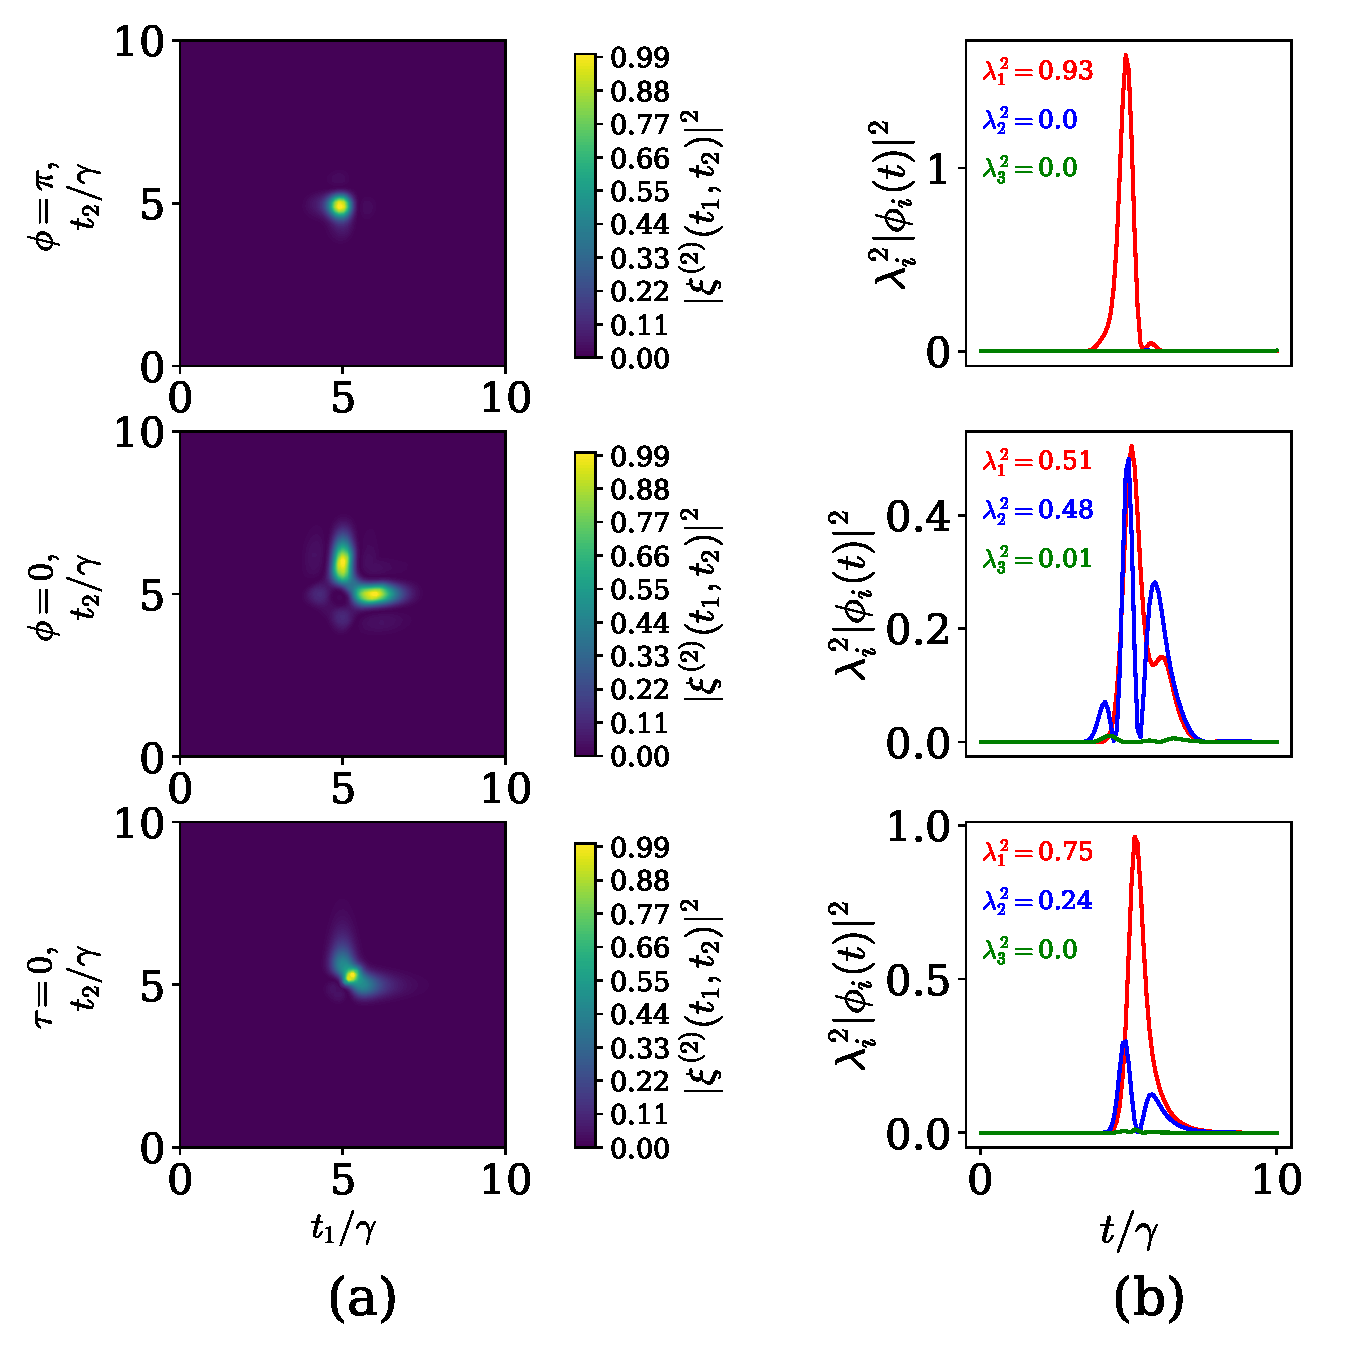
\includegraphics[width=\linewidth]{figures/twophoton_mirror.pdf}
    \caption{(a): The scattered two-photon Gaussian pulse for the same configuration and parameters  considered in Fig.~\ref{fig:tls_feedback} and \ref{fig:onephoton_pulse}. In the first row, the mirror phase is $\phi = \pi$, in the second row, it is $\phi=0$, and in the last row, we consider no delay $\tau=0$ (single-sided). All contour plots have been normalized so that the largest value is unity. (b): The SVD of the two-photon scattered state in (a). For $\phi=\pi$, we observe excitation trapping and thus $\sum_i \lambda_i^2 \neq 1$.}
    \label{fig:twophoton_mirror}
\end{figure}

\chapter{Conclusion and outlook}
In conclusion, we have in this Msc.~thesis successfully implemented the numerical framework \href{https://github.com/qojulia/WaveguideQED.jl}{WaveguideQED.jl} for simulating waveguide Quantum Electrodynamics (QED) problems. The tool is built on top of the QuantumOptics.jl library and maintains the excellent user experience offered by the original library. Through convergence studies, we have demonstrated the accuracy of the framework, ensuring that it produces correct results. Additionally, to enhance performance, we have introduced LazyOperators and discussed efficient representations of the waveguide state. 

By utilizing \href{https://github.com/qojulia/WaveguideQED.jl}{WaveguideQED.jl}, we have studied the scattering of two-photon pulses on a cavity and an emitter, reproducing recent experimental results. We demonstrate the non-linear capabilities of a single-emitter by showing that a scattered two-photon pulse has signatures of entanglement across time due to stimulated emission. On the contrary, scattering a two-photon pulse on a cavity does not lead to entanglement across time, only producing a product state, revealing that the photons effectively did not interact. Furthermore, we have described internal waveguide coupling and shown how to successfully model a defect in a waveguide leading to partial reflection of one waveguide mode into another. We show that such a defect changes the emission frequency and rate of a coupled emitter due to variations in the local density of optical states. We also predict the emergence of Fano resonances under certain parameter conditions of this scattering element. Finally, we demonstrated the framework's capability to treat non-Markovian dynamics by considering a semi-infinite waveguide with a mirror in one end. The emitted light is here fed back into the system leading to a complex feedback loop. We observe excitation trapping for a mirror phase of $\phi = \pi$, confirming other theoretical results. We extend those studies by considering how single- and two-photon pulses scatter on the system, where we no longer observe excitation trapping.

\

In essence, we have presented a versatile simulation tool that offers researchers in the field of quantum optics a simple but powerful approach. The software interface is intuitive and will be familiar to those already experienced with quantum optics software such as Qutip in Python, Quantum Toolbox in MATLAB, or QuantumOptics.j in Julia. By describing the total state of the waveguide without relying on matrix-product states, our simulation tool reduces the knowledge-barrier-to-entry, providing a transparent approach that is less of a black box. This allows for the exploration of non-Markovian dynamics while still maintaining an accessible framework. It is important to note that this comes with limitations, and specifically, it is, as of now, only possible to describe up to two photons simultaneously. Although it is, in principle, possible to extend the capabilities to allow for a larger number of photons, it comes at a significant numerical cost. In such cases, employing matrix product states might still be a better solution at the cost of complexity. 

\

Looking ahead, future work involves investigating the impact of non-Markovian dynamics on the preparation and alteration of exotic photonic states.  For example, 2D photonic cluster states from waveguides with feedback have been proposed \cite{Pichler2016PhotonicFeedback}. Recently, it was also studied how a single emitter can perform a two-photon splitting operation \cite{Lund2023PerfectPulse}. It is here interesting to consider if any advantage can be gained by introducing non-markovian dynamics or whether other schemes can be derived from such configurations. Furthermore, the optimization of schemes performing nonlinear operations on the photonic state is also a promising direction. Indeed, the framework is based on an analytical approach, which has already been employed to optimize C-phase gates by considering different nonlinearities \cite{Heuck2020Photon-photonCavities,Heuck2020Controlled-PhaseNonlinearities,Krastanov2022Controlled-phaseEmitter}. It is here possible that by using the numerical framework one can extend the analysis to more complex systems. Finally, the approach could also help to solve few-photon transport problems in more complex waveguide QED systems. Again, previous analysis has been performed using analytically derived scattering matrices \cite{Joanesarson2020Few-photonGeometries}, and with a numerical approach, it is possible to imagine the study of more complex systems.


\newpage
\appendix
\begin{appendices}
\chapter{Analytical derivations} \label{app:A}
\section{Rotating frame \label{app:rotating}}
In the quantum optical collision formalisms, the Hamiltonian is transformed into an interaction picture to introduce the notion of time bins. We consider the general Hamiltonian for $N$ waveguides interacting with a local quantum system $H_s$ with the annihilation operator $a$ (for an emitter system this would instead be $\sigma$) \cite{Xu2016FanoTransport}:
\begin{equation}
\begin{aligned}
H= H_{\mathrm{s}}+ \sum_{i=1}^N \int d \nu \hbar \nu w_{i}^{\dagger}(\nu) w_{i}(\nu)+\sum_{i=1}^N \hbar \sqrt{\gamma_i} \int \frac{d \nu}{\sqrt{2 \pi}}\left(w_{i}^{\dagger}(\nu) a+a^{\dagger} w_{i}(\nu)\right) +\sum_{i \neq j} \hbar 
 V_{i j} \int \frac{d \nu}{\sqrt{2 \pi}} \int \frac{d  \nu^{\prime}}{\sqrt{2 \pi}} w_{i}^{\dagger}(\nu) w_{j}(\nu^\prime),
\end{aligned}
\end{equation}
where $w_{i}(\nu)$ is the annihilation operator for a mode in waveguide $i$ with frequency $\nu$, $\gamma_i$ is the coupling between the local system and waveguide $i$, and $V_{i,j} =V_{j,i}$ is the coupling between waveguides. If we move into an interaction picture with regards to $H_0 =\hbar \omega_s a^\dagger a + \hbar 
 \sum_{i=1}^N \int d \nu \nu w_{i}^{\dagger}(\nu) w_{i}(\nu)$, the waveguide operators transform as:
\begin{equation}
    \mathrm{e}^{i H_0 t/\hbar } w_i(\nu) \mathrm{e}^{-i H_0 t/\hbar } = w_i(\nu) - i t \nu w_i(\nu) + 
    \frac{(-it\nu)^2}{2!} w_i(\nu) + \cdots = w_i(\nu) \mathrm{e}^{-i\nu t}
\end{equation}
and the system operators likewise as:
\begin{equation}
    \mathrm{e}^{i H_0 t/\hbar } a \mathrm{e}^{-i H_0 t/\hbar } = a \mathrm{e}^{-i \omega_s t}
\end{equation}
In the interaction picture, the transformed Hamiltonian $\Tilde{H}$ then becomes \cite{Breuer2006TheSystems}:
\begin{align}
\Tilde{H} = \mathrm{e}^{i H_0 t/\hbar } H \mathrm{e}^{-i H_0 t/\hbar } - H_0 &= H_{\mathrm{s}} - \hbar \omega_s a^\dagger a +\sum_{i=1}^N \hbar \sqrt{\gamma_i} \int \frac{d \nu}{\sqrt{2 \pi}}\left(w_{i}^{\dagger}(\nu) \mathrm{e}^{i(\nu - \omega_s) t} a+a^{\dagger} w_{i}(\nu) \mathrm{e}^{-i(\nu - \omega_s) t}\right)  \\
&+ \sum_{i \neq j} \hbar V_{i j} \int \frac{d \nu}{\sqrt{2 \pi}} \int \frac{d  \nu^{\prime}}{\sqrt{2 \pi}} w_{i}^{\dagger}(\nu) \mathrm{e}^{i\nu t} w_{j}(\nu^\prime) \mathrm{e}^{-i\nu^\prime t},
\end{align}
If we introduce the Fourier transformed waveguide operator $w_i(t) =\int \frac{d \nu}{\sqrt{2 \pi}} w_{i}(\nu) \mathrm{e}^{-i(\nu - \omega_s) t}$ the above simplifies to:
\begin{align}
\Tilde{H} = H_{\mathrm{s}}-\hbar \omega_s a^\dagger a+\sum_{i=1}^N \hbar \sqrt{\gamma_i} \left(w_{i}^{\dagger}(t) a+a^{\dagger} w_{i}(t)\right) + \sum_{i \neq j} \hbar V_{i j} w_{i}^{\dagger}(t) w_{j}(t), \label{eq:general_h}
\end{align}
Notice that for the waveguide interaction term, we inserted $\mathrm{e}^{-i \omega_s t}\mathrm{e}^{i \omega_s t} = 1$. Also, we see that the waveguide pulse has a frequency centered around $\omega_s$. If we instead wanted to describe a waveguide pulse centered around $\omega_w$ and a system with frequency $\omega_s$ we would transform using $H_0 =\hbar \omega_w a^\dagger a + \sum_{i=1}^N \int d \nu \hbar \nu w_{i}^{\dagger}(\nu) w_{i}(\nu)$ which would lead to a term like $\delta a^\dagger a$ in the system Hamiltonian $H_s$, where $\delta = \omega_s - \omega_w$.

In the collision framework, we then interpret equation \eqref{eq:general_h} as describing an interaction with photon bins. This can be understood by considering how the unitary evolution operator evolving from a time $t_{n-1}$ to a time $t_n$ where $t_n - t_{n-1} = \Delta t$ looks like:
\begin{align}
    U(t_{n-1},t_n) &= \exp \left (-i \int_{t_{n-1}}^{t_n} \mathrm{d}t^\prime H_{\mathrm{s}}-\omega_s a^\dagger a+\sum_{i=1}^N \sqrt{\gamma_i} \left(w_{i}^{\dagger}(t^\prime) a+a^{\dagger} w_{i}(t^\prime)\right) + \sum_{i \neq j} V_{i j} w_{i}^{\dagger}(t^\prime) w_{j}(t^\prime) \right ) \\
    &
\end{align}
If we now introduce a discretized operator $w_{n,i} = \frac{1}{\sqrt{\Delta t}} \int_{t_{n-1}}^{t_n} \mathrm{d}t^\prime w_{i}(t^\prime)$ that satisfies the commutation relation: $\comm{w_{n,i}}{w_{n^\prime,j}^\dagger} =  \frac{1}{\Delta t} \int_{t_{n-1}}^{t_n} \mathrm{d}t^\prime \int_{t_{n^\prime-1}}^{t_n^\prime} \mathrm{d}t^{\prime \prime} \comm{w_i(t^\prime)}{w_j(t^{\prime \prime})} =  \frac{1}{\Delta t} \int_{t_{n-1}}^{t_n} \mathrm{d}t^\prime \int_{t_{n^\prime-1}}^{t_n^\prime} \mathrm{d}t^{\prime \prime} \delta(t^\prime - t^{\prime \prime}) \delta_{i,j} = \delta_{n,n^\prime} \delta_{i,j}$, we can write the evolution operator as (we assume that the system Hamiltonian is time-independent for the sake of simplicity, but it is by no means a requirement):
\begin{align}
    U(t_{n-1},t_n) &= \exp \left (-i \Delta t H_{\mathrm{s}}-\Delta t \omega_s a^\dagger a\mathrm{d}t^\prime + \sqrt{\Delta t} \sum_{i=1}^N \sqrt{\gamma_i} \left(w_{n,i}^{\dagger} a+a^{\dagger} w_{n,i} \right) + \Delta t \sum_{i \neq j} V_{i j} w_{n,i}^{\dagger} w_{n,j} \right ) \\
\end{align}
Notice that if we take the $\Delta t$ outside, we get:
\begin{align}
    U(t_{n-1},t_n) &= \exp \left (-i \Delta t \left [ H_{\mathrm{s}}- \omega_s a^\dagger a\mathrm{d}t^\prime + \sum_{i=1}^N \sqrt{\gamma_i/\Delta t} \left(w_{n,i}^{\dagger} a+a^{\dagger} w_{n,i} \right) + \sum_{i \neq j} V_{i j} w_{n,i}^{\dagger} w_{n,j} \right ] \right ) \\
\end{align}
We thus have a rescaled Hamiltonian:
\begin{equation}
    H_{\mathrm{s}}- \hbar \omega_s a^\dagger a  + \sum_{i=1}^N \hbar 
 \sqrt{\gamma_i/\Delta t} \left(w_{n,i}^{\dagger} a+a^{\dagger} w_{n,i} \right) + \sum_{i \neq j}\hbar  V_{i j} w_{n,i}^{\dagger} w_{n,j}
\end{equation}
that leads to a constant evolution within each time bin. We could also have arrived at this Hamiltonian by introducing the discretized operators as  a transformation of the continuous: $w(k \Delta t) \rightarrow  \frac{w_k}{\sqrt{\Delta t}}$.

If we rescale $V_{ij}$, we see that we recover the beamsplitter transformation. One caveat, however, applies, since we made the following approximation when we discretized the interaction:
\begin{equation}
    \int_{t_{n-1}}^{t_n} w_i^\dagger(t^\prime) w_j(t^\prime) \approx \int_{t_{n-1}}^{t_n} w_i^\dagger(t^\prime) \int_{t_{n-1}}^{t_n} w_j(t^\prime) = \Delta t w_{n,i}^\dagger w_{n,j}
\end{equation}
whether this approximation is accurate is not obvious, but we do see that we recover the unitary transformation of a beamsplitter with it. In sec. \ref{sec:waveguideIO} and \ref{sec:inferringwaveguide}, we discuss the possible problems with making this approximation and possible solutions to it. 





\section{Analytical solution to single-photon scattering \label{app:analytical}}

In sec. \ref{sec:onephoton_scat}, we derive the following differential equation for the scattering of a single photon on a cavity:  
\begin{equation}
    \frac{d \psi_1(t)}{d t}  = -(i \delta_a +\frac{\gamma}{2}) \psi_1(t) + \sqrt{\gamma} \xi^{(1)}(t)
\end{equation}
The general solution for this differential equation is given as \cite{Arfken2005MathematicalPhysicists}:
\begin{equation}
\psi_1(t) =  \mathrm{e}^{-(i\delta_a+\frac{\gamma}{2}) t} \left [ \psi_1(0) + \int_{0}^t \mathrm{e}^{-(i\delta_a+\frac{\gamma}{2}) t} \xi(s)  ds \right ]
\end{equation}
In sec. \ref{sec:onephoton_numerical}, we consider a Gaussian input state with $\xi^{(1)}(t) = \sqrt{\frac{2}{\sigma}} \left(\frac{\log(2)}{\pi}\right)^{1/4} \exp\left(-\frac{2\log(2)(t-t_0)^2}{\sigma^2}\right) $ and $\psi_1(0)=0$.
Inserting, we thus have the integral:
%\sqrt{\frac{2\gamma}{\sigma}}\left(\frac{\log 2}{\pi}\right)^{\frac{1}{4}}\exp\left[-\frac{2\log^2 2}{\sigma^2}(s-t_0)^2\right]
\begin{equation}
\psi_1(t) = \sqrt{\frac{2}{\sigma}}\left(\frac{\log(2)}{\pi}\right)^{\frac{1}{4}}\int_{0}^t e^{-(i\delta_a+\frac{\gamma}{2})t}\exp\left[-\frac{2\log(2)}{\sigma^2}(s-t_0)^2\right] ds
\end{equation}

Using,
\begin{equation}
    \int_{0}^{t} e^{-a(s-t_0)^2+b s}ds = \frac{\sqrt{\pi} e^{\frac{b^2}{4a}+bt_0}}{2\sqrt{a}}\left(\text{erf}\left(\frac{2a(t-t_0)-b}{2\sqrt{a}}\right) + \text{erf}\left(\frac{2at_0+b}{2\sqrt{a}}\right)\right)
\end{equation}
together with the input-output relation $\xi_{out}(t) = \xi_{in}(t) - \sqrt{\gamma}\psi(t)$ we get:
\begin{equation}
    \xi^{(1)}_\mathrm{out}(t) =  \xi_{in}^{(1)}(t) - \sqrt{\gamma} \frac{\sqrt{\pi} e^{\frac{b^2}{4a}+bt_0}}{2\sqrt{a}}\left(\text{erf}\left(\frac{2a(t-t_0)-b}{2\sqrt{a}}\right) + \text{erf}\left(\frac{2at_0+b}{2\sqrt{a}}\right)\right)
\end{equation}
with $a = 2 \log(2)/\sigma^2$ and $b = i \delta + \gamma/2$. Which is also the result in eq. \eqref{eq:onephoton_analytical}.



\section{Waveguide Interaction \label{app:waveguideinteraction}}
In chapter \ref{ch3}, we consider how multiple waveguides interact, and in this appendix, we elaborate on some of the derivations. We consider two waveguides labeled $a$ and $b$, which interact through the following Hamiltonian:
\begin{equation}
     H_{int}(t) = \sum_k f_k(t) H_k = \sum_k f_k(t) \frac{\hbar V}{\Delta t}\left(w_{k, a}^{\dagger} w_{k, b}+w_{k, b}^{\dagger} w_{k, a}\right)= \sum_k f_k(t)\frac{\hbar V}{\Delta t} O_k
\end{equation}
where $f_k(t)$ is as defined as in eq. \eqref{eq:fk} and $O_k = \left(w_{k, a}^{\dagger} w_{k, b}+w_{k, b}^{\dagger} w_{k, a}\right)$. We notice that $\comm{H_{int}(t)}{w_{k,a/b}} = 0$ unless $t_k<t <t_k +\Delta t$. The equation of motion of the operators $w_{k,a}$ and $w_{k,b}$ are thus:
\begin{equation}
    \frac{d w_{k,a/b}}{d t} = \begin{cases}
           - \frac{i}{\hbar}\comm{w_{k,b}}{\frac{\hbar V}{\Delta t} O_k} , & \text{if } t_k < t <t_k+\Delta t  \\
          0, & \text{otherwise}
\end{cases}
\end{equation}
Thus for all times $t<t_k$ where have $w_{k,a/b}(t) = w_{k,a/b}$, while after the time window of $t_k < t <t_k+\Delta t$ the evolution is given by the unitary operator:
\begin{equation}
    U(t_k,t_k+\Delta t) =\exp \left[-\frac{i}{\hbar} \int_{t_k}^{t_k+\Delta t} H_{\mathrm{int}}(t^\prime) d t^{\prime}\right] = \exp \left[-\frac{i}{\hbar} 
\Delta t \frac{\hbar V}{\Delta t} O_k \right] = \exp \left[-i V O_k \right] 
\end{equation}
we thus have that the operator $w_{k,a}(t_k + \Delta t)$ after the interaction (where the derivative is zero and it no longer changes) is:
\begin{equation}
    w_{k,a}(t_k + \Delta t) = U^\dagger(t_k,t_k+\Delta t) w_{k,a} U(t_k,t_k+\Delta t)  = \exp \left[i V O_k \right]  w_{k,a} \exp \left[-i V O_k \right] 
\end{equation}
We can then use the Baker-Hausdorf lemma \cite{Gerry2004IntroductoryOptics}: 
\begin{equation}
   \mathrm{e}^{i \lambda A} B \mathrm{e}^{-i \lambda A} = B + i \lambda [A,B] + \frac{(i \lambda)^2}{2!}[A,[A,B]] + \frac{(i \lambda)^3}{3!}[A,[A,[A,B]]] + ...
\end{equation}
together with the following commutators:
\begin{align}
    &\comm{O}{w_{k,a}} = \left[w_{k, a}^\dagger w_{k, b}+w_{k, b}^{\dagger} w_{k, a}, w_{k, a}\right] = \left[w_{k, a}^{\dagger} w_{k, b}, w_{k, a}\right]=\left[w_{k, a}^\dagger, w_{k, a}\right] w_{k, b} = -w_{k, b} \\
    & \comm{O}{w_{k,b}} = -w_{k, a}
\end{align}
which gives:
\begin{align}
     w_{k,a}(t_k + \Delta t) & = w_{k,a} - i V w_{k,b} + \frac{(i V)^2}{2 !} w_{k,a}-\frac{(i V)^3}{3!} w_{k,b}+\cdots \\
    & = w_{k,a}(1 - \frac{V^2}{2!} + \cdots ) + w_{k,b}(-iV + i \frac{V^3}{3!} + \cdots ) = \cos(V) w_{k,a} -i \sin(V) w_{k,b}
\end{align}
and similarly:
\begin{align}
    w_{k,b}(t_k + \Delta t) = \cos(V) w_{k,b} -i \sin(V) w_{k,a}
\end{align}

Notice that if we instead had chosen the interaction Hamiltonian: 
\begin{equation}
     H_{int}(t) = \sum_k f_k(t) \frac{\hbar i V}{\Delta t}\left(w_{k, b}^{\dagger} w_{k, a} - w_{k, a}^{\dagger} w_{k, b}\right) = \sum_k f_k(t)\frac{i \hbar V}{\Delta t} Q_k
\end{equation}
with $Q_K =  w_{k, b}^{\dagger} w_{k, a} - w_{k, a}^{\dagger} w_{k, b}$ and consequently $\comm{Q_k}{w_{k,a}} = - w_{k,b}$ and $\comm{Q_k}{w_{k,b}} = w_{k,b}$ , which would then give:
\begin{equation}
    w_{k,a}(t_k + \Delta t) = \exp \left[- V Q_k \right]  w_{k,a} \exp \left[V Q_k \right] = w_{k,a} + V - \frac{V^2}{2!}w_{k,a} - \frac{V^3}{3!}w_{k,b} = \cos(V) w_{k,a} + \sin(V) w_{k,b}   
\end{equation}
\begin{equation}
    w_{k,b}(t_k + \Delta t) =  \cos(V) w_{k,b} - \sin(V) w_{k,a}   
\end{equation}


\

We can derive similar input-output relations for the more general case where we interact with a quantum system with an arbitrary number of waveguides. We write the general Hamiltonian in eq. \eqref{eq:general_transformed} as: 
\begin{equation}
\begin{aligned}
H_k = H_{s} + H_{k,sb} + H_{k,b} \label{eq:generalinteraction}
\end{aligned}
\end{equation}
where $H_{s}$ is Hamiltonian of the quantum system Hamiltonian, $H_{k,sb} = \sum_{i=1}^N \hbar \sqrt{\gamma_i/\Delta t} \left(w_{k,i}^{\dagger} a+a^{\dagger} w_{k,i} \right)$ the interaction with the system, where $a$ is the annihilation of the quantum system (for a two-level system, $\sigma$ would be a more appropriate symbol), and $\gamma_i$ defines the interaction strength between the quantum system and the corresponding waveguide mode $i$. $ H_{k,b} = \sum_{i \neq j} \hbar  V_{i j}/\Delta t w_{k,i}^{\dagger} w_{k,j}$ defines the interaction between the waveguides modes $i$ and $j$. The time-evolution operator is now given as:
%Note that the form of eq. \eqref{eq:generalinteraction} requires $V_{\mu,\nu} = - V_{\nu,\mu}$ for there to be time-reversal symmetry. In addition, it is shown in ref. \cite{Xu2016FanoTransport} that a Hamiltonian of similar form also ensures flux conservation, energy conservation, and causality.
\begin{equation}
    U(t_k,t_k+\Delta t) =\exp \left[-\frac{i}{\hbar} \int_{t_k}^{t_k+\Delta t} [ H_s + H_{sb} + H_b ] d t^{\prime}\right] = \mathrm{e}^{ \left[ -i \Delta t / \hbar [ H_s + H_{sb} + H_b ] \right ]}
\end{equation}

This form is much more complicated and will, in general, lead to complex self-energy corrections, this is clear if we expand the above exponential using the Zassenhaus formula (in the following we omit a factor of $\Delta t/\hbar$ and absorb it into a normalized Hamiltonian $\Tilde{H} = \Delta t/\hbar H$):

\begin{align}
    U(t_k,t_k+\Delta t) &= \mathrm{e}^{ -i [ \Tilde{H}_s + \Tilde{H}_{sb} + \Tilde{H}_b ]} = \mathrm{e}^{ -i \Tilde{H}_b } \mathrm{e}^{ -i [ \Tilde{H}_{s} + \Tilde{H}_{sb}]} \mathrm{e}^{ 1/2 \comm{\Tilde{H}_b}{\Tilde{H}_{sb}}} \mathrm{e}^{ i/6  \comm{\Tilde{H}_b}{\comm{\Tilde{H}_b}{\Tilde{H}_{sb}}}} \mathrm{e}^{ -1/24 \comm{\comm{\comm{\Tilde{H}_{sb}}{\Tilde{H}_b}}{\Tilde{H}_b}}{\Tilde{H}_b}}\cdots \\
    &= \mathrm{e}^{ -i \Tilde{H}_b } \mathrm{e}^{ -i [ \Tilde{H}_{s} + \Tilde{H}_{sb}]} \mathrm{e}^{-i \Tilde{H}_{eff}} 
\end{align}
where it was used that $\comm{H_b}{H_s} = 0$ and also that $\comm{H_b}{H_{bs}}$ will only generate terms of the type $a w_{k,\mu}^\dagger$ and $a^\dagger w_{k,\mu}$ and so  $\comm{\comm{H_b}{H_{bs}}}{H_{bs}} = 0$. The infinite series will serve as a self-energy correction to the waveguide-system interaction $H_{eff}$, but the input-output relation will still just be given by $\mathrm{e}^{-\Tilde{H_b}}$. The input-output relation can be calculated from the commutator:
\begin{equation}
    \comm{w_{k,\mu}}{H_b} = \sum_{\nu \neq \mu} - i/\Delta t V_{\mu,\nu} w_{k,\nu}
\end{equation}
if we introduce the vector $\textbf{W} = \begin{pmatrix}
    w_{k,1} \\ w_{k,2} \\ \vdots \\ w_{k,N}
\end{pmatrix}$ where $N$ is the number of waveguides, and $\textbf{V} = \begin{pmatrix}
    0 & V_{1,2} & \cdots & V_{1,N} \\
    V_{2,1} & 0 & \cdots & V_{2,N} \\
     \vdots & \vdots & \ddots & \vdots \\
     V_{N,1} & V_{N,2} & \cdots & 0 \\
\end{pmatrix}$ we can write all commutator relations as:
\begin{equation}
    \comm{\textbf{W}}{H_b} = - i/\Delta t \textbf{V} \textbf{W}
\end{equation}
and the waveguide operators thus transform unitary evolution as:
\begin{equation}
    \mathrm{e}^{i \Delta t H_b} \textbf{W} \mathrm{e}^{-i \Delta t H_b} = \textbf{W} + i \Delta t\comm{H_b}{\textbf{W}} - \frac{\Delta t^2}{2!} \comm{H_b}{\comm{H_b}{\textbf{W}}} + \cdots = \textbf{W} + \textbf{V} \textbf{W} + \textbf{V}^2/2! \textbf{W} + \cdots = \exp(\textbf{V}) \textbf{W}  
\end{equation}
and we will thus have the total transformation:
\begin{align}
    U(t_k,t_k+\Delta t)^\dagger \textbf{W} U(t_k,t_k+\Delta t) &=  \mathrm{e}^{i \Tilde{H}_{eff}} \mathrm{e}^{ i [ \Tilde{H}_{s} + \Tilde{H}_{sb}]}  \mathrm{e}^{ i \Tilde{H}_b } \textbf{W} \mathrm{e}^{ -i \Tilde{H}_b } \mathrm{e}^{ -i [ \Tilde{H}_{s} + \Tilde{H}_{sb}]} \mathrm{e}^{-i \Tilde{H}_{eff}} \\
    &= \mathrm{e}^{-i \Tilde{H}_{eff}} \mathrm{e}^{ -i [ \Tilde{H}_{s} + \Tilde{H}_{sb}]}  \exp(\textbf{V}) \textbf{W} \mathrm{e}^{ -i [ \Tilde{H}_{s} + \Tilde{H}_{sb}]} \mathrm{e}^{-i \Tilde{H}_{eff}}
\end{align}
We thus see that if we did not have any local system, the waveguide operators would transform as $\textbf{W}_{out} = \textbf{W}(t+\Delta t) = \textbf{C} \textbf{W}(t)$ with $\textbf{C}=\exp(\textbf{V})$.







\chapter{Code} \label{app:B}
\section{Two-photon routine \label{app:twophotonroutine}}
The following shows the two-photon annihilation routine. Lines 1-9 are equivalent to the one-photon routine to perform actions like $w_k \ket{1_k} = \ket{\emptyset}$. Line 10 calls, \code{twophoton\_destroy!}, which in lines 14-16 loop horizontally over the two-photon state (see fig. \ref{fig:twophoton_representation}). Similarly, lines 17-19 loop vertically, while lines 21-22 treat the special case of the diagonal, where a factor of $\sqrt{2}$ has to be applied.  

\begin{listing}[H]
\begin{minted}[
frame=lines,
framesep=2mm,
baselinestretch=1.2,
bgcolor=LightGray,
fontsize=\small,
linenos,
escapeinside=||,
mathescape=true
]{julia}
function waveguide_mul!(result,a::WaveguideDestroy{B,B,2,1},b,alpha,beta) where {B}
    if iszero(beta)
        fill!(result, beta)
    elseif !isone(beta)
        rmul!(result, beta)
    end
    timeindex = a.timeindex
    nsteps = a.basis_l.nsteps
    @inbounds result[1] += alpha*a.factor*b[timeindex+1]
    twophoton_destroy!(view(result,2:1:nsteps+1),b,alpha*a.factor,timeindex,nsteps,nsteps+1)
    return
end
function twophoton_destroy!(result,b,alpha,timeindex,nsteps,offset)
    @simd for i in 1:timeindex-1
        @inbounds result[i]  += alpha*b[offset + twophoton_index(i,nsteps,timeindex)]
    end
    @simd for i in timeindex+1:lastindex(result)
        @inbounds result[i]  += 
        alpha*b[offset + twophoton_index(timeindex,nsteps,i)]
    end
    @inbounds result[timeindex] += sqrt(2)*alpha*b[offset +
    twophoton_index(timeindex,nsteps,timeindex)]
end
\end{minted}
\caption{Code for the two-photon annihilation multiplication routine. }
\label{ls:twophoton_routine}
\end{listing}

\section{Lazy Tensor routine \label{app:lazytensor}}
The following recursive loop shows the main principle behind how the LazyTensor routine is run. 
\begin{listing}[H]
\begin{minted}[
frame=lines,
framesep=2mm,
baselinestretch=1.2,
bgcolor=LightGray,
fontsize=\small,
linenos,
escapeinside=||,
mathescape=true
]{julia}
function recursive_tensor(result,op,input,alpha,beta,N,dim,i_operator,I,strides,shape)
    if dim<N+1
        if dim != i_operator
            for j in 1:shape[dim]
                J += strides[dim]*(j-1)
                return recursive_tensor(result,op,input,N,dim+1,i_operator,I,strides,shape)
            end
        return recursive_tensor(result,op,input,alpha,beta,N,dim+1,i_operator,I,strides,shape)
    end
    mul!(view(result,I:strides[i_k]:I+strides[i_k]*(shape[i_k]-1)),
    op.operators[i_operator],
    view(input,I:strides[i_k]:I+strides[i_k]*(shape[i_k]-1)),alpha,beta)
end 
\end{minted}
\caption{Code that demonstrates the main principle of the LazyTensor recursive loop. }
\label{ls:lazy_routine}
\end{listing}
The counter \code{dim} keeps track of the current dimension and is incremented throughout the recursive loop, to go over all dimensions. When we have looped over all dimensions \code{dim = N+1}, and we proceed to the last part of the code, where the multiplication is performed. \code{i\_operator} is the index of the operator applied being applied. \code{shape} contains the sizes of the sub-Hilbert spaces

\section{Convergence of two-photon scattering \label{app:twophoton_convergence}}
In sec. \ref{sec:twophoton_emitter_vs_cavity}, we consider scattering of a two-photon pulse on a cavity and emitter. For the scattering of the cavity, we can confirm the numerical results by doing a convergence study between the equations of motion in eq. \eqref{eq:twophotonEOM} and the numerical approach. The equations of motion in eq. \eqref{eq:twophotonEOM} are also discretized because the two-time functions $\psi_1^{(0)}(t_m,t_n)$ and $\psi_1^{(1)}(t_m,t_n)$ has to be solved for each $t_m = 0$, $t_m = \Delta t$, $t_m = 2\Delta t$, and so on. If we choose the same discretization $\Delta t$ for the equations of motion and the numerical approach, we see in Fig. \ref{fig:twophoton_convergence} that the two methods already agree very well for large $\Delta t$'s (probably because they are both discretized), but as $\Delta t$ the error decreases even further.

\begin{figure}[H]
    \centering
    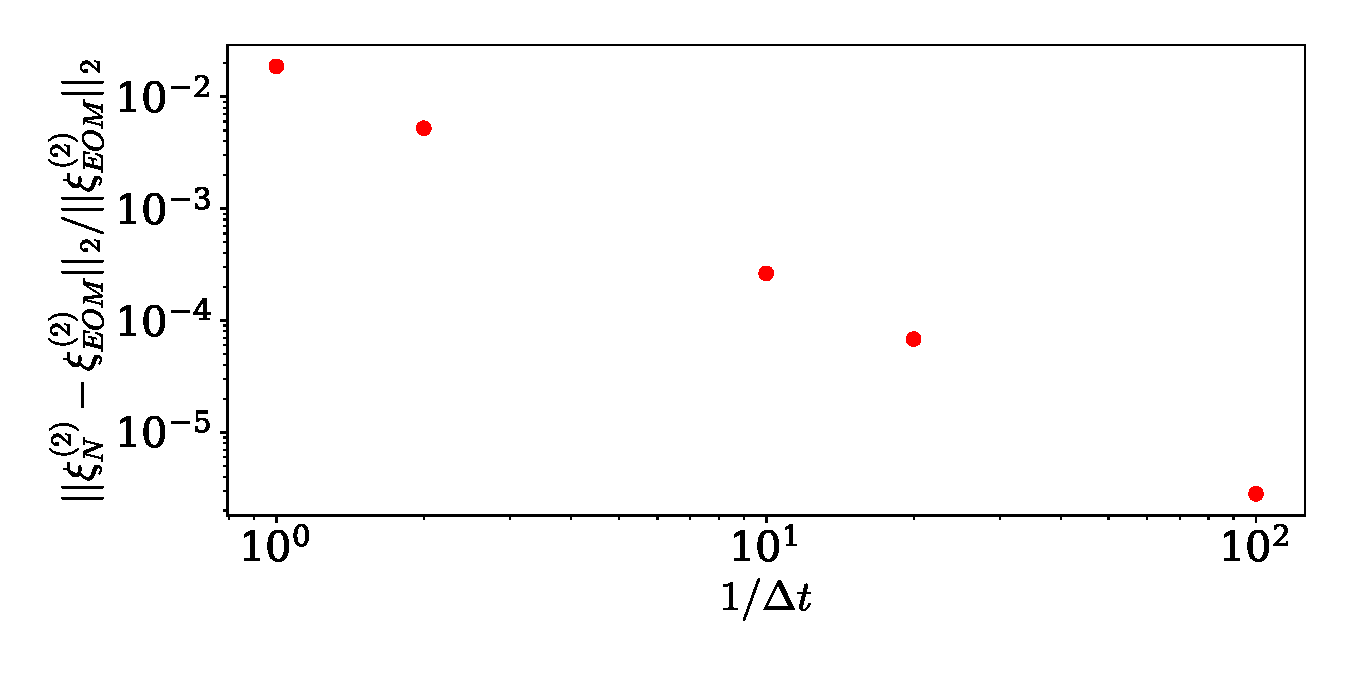
\includegraphics[width=0.5 \linewidth]{figures/twophoton_convergence.pdf}
    \caption{Relative error between the scattered two-photon wavefunction $\xi_N$ and equations of motions wavefunction $\xi_{EOM}$ for different values of $\Delta t$. We here defined the norm: $|f|_2 = \int dt \int dt' f(t,t')$.}
    \label{fig:twophoton_convergence}
\end{figure}




\end{appendices}

\bibliography{references}
\bibliographystyle{ieeetr}
\label{endOfDoc}

\end{document}
